\documentclass[11pt]{article}
\usepackage{cmap}
\usepackage[T1]{fontenc}
\usepackage[utf8]{inputenc}
\usepackage[sc]{mathpazo}
\linespread{1.05}
\usepackage[a4paper,margin=26mm]{geometry}
\usepackage{amsmath,amssymb,amsthm,mathtools,booktabs,array,longtable,graphicx,xcolor,enumitem,microtype}
\usepackage[hidelinks,pdftitle={Arithmetic Occurrence Geometry in the UNNS Substrate: Exceptional Topology and Universal Convex Stabilization},pdfauthor={UNNS Research Collective}]{hyperref}
\newcommand{\geoicommit}{\texttt{343f9aef\allowbreak 2b669746\allowbreak 6058165c\allowbreak 5fc2ddf0\allowbreak f00e882b}}
\usepackage[capitalise,noabbrev]{cleveref}
\usepackage{caption}
\captionsetup{font=small,labelfont=bf}
\setlist{itemsep=2pt,topsep=3pt}
\setlength{\emergencystretch}{3em}

\newtheorem{theorem}{Theorem}[section]
\newtheorem{lemma}[theorem]{Lemma}
\newtheorem{proposition}[theorem]{Proposition}
\newtheorem{corollary}[theorem]{Corollary}
\theoremstyle{definition}
\newtheorem{definition}[theorem]{Definition}
\newtheorem{example}[theorem]{Example}
\theoremstyle{remark}
\newtheorem{remark}[theorem]{Remark}
\newtheorem{question}{Question}

\newcommand{\Z}{\mathbb Z}
\newcommand{\R}{\mathbb R}
\newcommand{\Q}{\mathbb Q}
\newcommand{\conv}{\operatorname{conv}}
\newcommand{\interior}{\operatorname{int}}
\newcommand{\cross}{\operatorname{cr}}
\newcommand{\ord}{\operatorname{ord}}
\newcommand{\conf}{\sqsubseteq}
\newcommand{\src}[1]{\par\smallskip\noindent{\footnotesize\textit{Source status.} #1\par}\smallskip}
\newcommand{\figdesc}[1]{\textit{Description:} #1}
\crefname{theorem}{Theorem}{Theorems}
\crefname{lemma}{Lemma}{Lemmas}
\crefname{proposition}{Proposition}{Propositions}
\crefname{corollary}{Corollary}{Corollaries}
\crefname{definition}{Definition}{Definitions}
\crefname{example}{Example}{Examples}
\crefname{remark}{Remark}{Remarks}

\title{Arithmetic Occurrence Geometry in the UNNS Substrate:\\
Exceptional Topology and Universal Convex Stabilization\\[2pt]
\large Modular Relation Lattices, Graver-Cell Realizations, and Constructive Coverage Theorems}
\author{UNNS Research Collective\thanks{UNNS Substrate Research Program, \texttt{unns.tech}. GEO-I Manuscript~I.}}
\date{28 October 2026}

\newcommand{\statTotal}{366}\newcommand{\statInterior}{241}\newcommand{\statWord}{366}
\begin{document}
\maketitle

\begin{abstract}
\noindent Distinct occurrences of a common value in the UNNS nest arithmetic are pairs $(N,M)$ of positive integers with $x=M(N+1)^2/N$. For a reduced rational $x=a/b$ these occurrences correspond, exactly and bijectively, to the nonzero points of a congruence lattice $\Lambda_b$ inside a box of prime-exponent vectors. When two prime coordinates are active, a positive diagonal change of coordinates turns $\Lambda_b$ into the modular lattice $\Gamma_{d,s}=\{(i,j):j\equiv si \pmod d\}$. On such a normalized fibre we study the \emph{realized union} $U_Q$ of all parallelograms and segments spanned by conformally minimal (Graver) lattice vectors with corners in the punctured fibre $F_Q$ of a box $Q$.

We prove: (i) in the minimal box $Q=(d,d)$ the complement of $U_Q$ in the convex hull $H_Q$ is exactly two open triangles for every unit $s\not\equiv-1 \pmod d$ with $d\ge 3$ (so $\beta_1=2$), while for $s\equiv-1$ the realized union is a fan graph with $\beta_1=d$; (ii) these holes are filled by explicit Graver parallelograms as soon as the box is enlarged; (iii) an arithmetic inequality for Pareto-minimal lattice points and a reflection lemma for boundary Graver steps give an explicit cell family covering the whole cap $H_Q\setminus H_{(d,d)}$ of every small enlargement; and (iv) consequently $U_{d,s,Q}=\conv(F_{d,s,Q})$ for every $d\ge2$, every unit $s$ and every integer box with $Q_1,Q_2\ge d$, $Q\neq(d,d)$. The transition is illustrated on the explicit occurrence fibres of $5^{10}3^{10}/11$ (two holes) and $5^{12}3^{10}/11$ (convex).

The results are proved for the planar normalized family and, through the normalization, for actual two-prime occurrence fibres; they say nothing about higher-dimensional fibres or about relations between different values. Universal statements are proved in the text; finite computations, independent tests and source-release certificates are described separately and are never used as proofs.
\end{abstract}

\medskip\noindent\textbf{Keywords:} occurrence arithmetic, congruence lattices, Graver basis, conformal minimality, parallelogram cells, zonogon, convex hull, Alexander duality.\\
\textbf{Mathematics Subject Classification (provisional, to be confirmed):} 11H06, 52C05, 52B20, 05B45.

\tableofcontents
\clearpage

%% ===================================================================
%% PART I
%% ===================================================================
\part{Arithmetic origin and geometric foundations}

\section{Introduction: from arithmetic occurrences to geometry}\label{sec:intro}

\subsection{The question}

In the nest arithmetic of the UNNS Substrate, a pair $(N,M)$ of positive integers has the \emph{value}
\begin{equation}\label{eq:value}
  x \;=\; M\,\frac{(N+1)^2}{N}.
\end{equation}
Different pairs can have the same value. A small example is $x=36$: the pairs $(1,9)$, $(2,8)$ and $(5,5)$ all satisfy \eqref{eq:value} with $x=36$, since $9\cdot 4/1=8\cdot 9/2=5\cdot 36/5=36$. We call each such pair an \emph{occurrence} of the value. Equality of values is therefore an arithmetic fact about numbers, while identity of occurrences is a finer fact about pairs. This paper is about the finite configuration formed by all occurrences of one value, and the question it answers is the following.

\begin{quote}
\emph{What geometric structure can be built on the exact arithmetic coordinates of the occurrences of a single value, and how does that structure change as the range of admissible occurrences grows?}
\end{quote}

The arithmetic part of the answer is short and exact (Section~\ref{sec:arith}). If $x=a/b$ in lowest terms and $\kappa=N+1$, the occurrences of $x$ are in bijection with the integers $\kappa\ge 2$ such that $\kappa^2\mid a$ and $\kappa\equiv 1 \pmod b$. Writing $\kappa$ in terms of the prime factorization of $a$ identifies these occurrences with the nonzero points of a congruence lattice inside a box of exponent vectors. When two primes are active the lattice is, after a positive diagonal change of coordinates, the \emph{modular lattice}
\[
  \Gamma_{d,s}\;=\;\{(i,j)\in\Z^2:\ j\equiv s\,i \pmod d\},\qquad \gcd(s,d)=1,
\]
and the occurrences of $x$ are its nonzero points in a box $[0,Q_1]\times[0,Q_2]$ (Section~\ref{sec:planar}).

The geometric part is a construction. Two occurrences are related by an exact multiplicative relation between their indices, and the minimal such relations are \emph{Graver vectors} of the lattice, that is, conformally minimal lattice vectors. Using only Graver vectors we attach to the occurrence points all parallelograms, segments and points that they span (Section~\ref{sec:cells}). The resulting compact set $U_Q$ is the \emph{realized union}. It lies inside the convex hull $H_Q$ of the occurrence points. The paper determines when, and how, $U_Q$ fills $H_Q$.

\subsection{Terminology: arithmetic occurrence geometry}\label{sec:terminology}

We use the term \emph{arithmetic occurrence geometry} for the study of distinct arithmetic occurrences of a common numerical value, their exact coordinate relationships, and geometric structures explicitly constructed upon those relationships. In the UNNS framework such occurrences are represented by finite arithmetic fibres obtained from prime-exponent coordinates and congruence relations (Section~\ref{sec:arith}); the resulting point configurations are the arithmetic foundation for constructions involving Graver generators, admissible cells, convex hulls, topological invariants and embedding properties. The occurrence coordinates are determined by arithmetic. The geometric cell constructions are separately specified mathematical structures: arithmetic occurrence geometry thus distinguishes the intrinsic organization of the occurrences from the properties of a particular geometric realization. The formal definition is Definition~\ref{def:aog}, placed directly after the derivation of the fibre $F_x$. The term is a defined term of this work; the scope note at the end of Section~\ref{sec:lit} says what it does not mean.

The companion manuscript, Paper~B (a separate manuscript released together with this one), studies embedding obstructions in a binary $0/1$ specialisation of the same Graver-cell construction.

\subsection{Main results}

Throughout, $d\ge 2$ is an integer, $s$ is an integer unit modulo $d$, $t\equiv s^{-1}\pmod d$, and $Q=(Q_1,Q_2)$ is an integer box with $Q_1,Q_2\ge d$. We write $F_Q=(\Gamma_{d,s}\cap[0,Q_1]\times[0,Q_2])\setminus\{0\}$, $H_Q=\conv F_Q$ and $U_Q\subseteq H_Q$ for the realized union, all defined precisely in Section~\ref{sec:cells}. The \emph{exceptional box} is $Q_0=(d,d)$; we write $H_0$ and $U_0$ for $H_{Q_0}$ and $U_{Q_0}$.

\begin{theorem}[Occurrence-coordinate correspondence; Theorem~\ref{thm:occ}]
For a reduced rational $x=a/b>0$, the occurrences of $x$ are in bijection with $D(x)=\{\kappa\ge2:\kappa^2\mid a,\ \kappa\equiv1 \pmod b\}$, and $D(x)$ is in bijection with $F_x=(\Lambda_b\cap[0,q])\setminus\{0\}$, where $\Lambda_b$ is the kernel of the homomorphism $\Z^k\to(\Z/b)^\times$, $\alpha\mapsto\prod_i p_i^{\alpha_i}$. When two prime coordinates are active, $\Lambda_b$ is the image of $\Gamma_{d,s}$ under a positive diagonal map for suitable $d\ge1$ and $s$, and the box is $\bigl(\lfloor q_1/\lambda_1\rfloor,\lfloor q_2/\lambda_2\rfloor\bigr)$.
\end{theorem}

\begin{theorem}[Exact exceptional complement; Theorem~\ref{thm:exceptional}]
Let $d\ge5$, $2\le s\le d-2$, $\gcd(s,d)=1$. Then
\[
  H_0\setminus U_0=\interior T_1\sqcup\interior T_2,
\]
where $T_1,T_2$ are two explicit lattice triangles of area $d/2$ with a common vertex $(d,d)$. In particular $U_0$ has exactly two bounded complementary components and $\beta_1(U_0)=2$. For $s\equiv 1$ and $d\ge3$ the same identity holds (Proposition~\ref{prop:special-plus}); for $s\equiv-1$ the set $U_0$ is a fan graph with $\beta_1(U_0)=d$ (Proposition~\ref{prop:special-fan}).
\end{theorem}

\begin{theorem}[Hole filling; Proposition~\ref{prop:fill}]
For $d\ge3$, every unit $s$ and every box $Q\ge(d,d)$ with $Q\ne(d,d)$, the closed triangles $T_1,T_2$ lie in $U_Q$. Consequently $H_0\subseteq U_Q$ whenever the complement of $U_0$ in $H_0$ is exactly the two open triangles.
\end{theorem}

\begin{theorem}[Universal planar convex stabilization; Theorem~\ref{thm:universal}]\label{thm:intro-main}
For every $d\ge 2$, every unit $s$ modulo $d$, and every integer box $Q$ with $Q_1,Q_2\ge d$ and $Q\ne(d,d)$,
\[
  \boxed{\,U_{d,s,Q}=\conv\bigl(F_{d,s,Q}\bigr).\,}
\]
\end{theorem}

\begin{corollary}[Actual fibres; Corollary~\ref{cor:actual}]
Let $x=a/b$ have two active prime coordinates with $d\ge2$, $q_i\ge o_i$ for $i=1,2$ and $(\lfloor q_1/\lambda_1\rfloor,\lfloor q_2/\lambda_2\rfloor)\neq(d,d)$. Then the realized Graver-cell union of the occurrence fibre of $x$ equals its convex hull, and is contractible. The excluded case $\lfloor q_i/\lambda_i\rfloor=d$ is an arithmetic plateau $o_i\le q_i\le o_i+\lambda_i-1$, and there the union has exactly the topology described by the exceptional complement theorem.
\end{corollary}

For the pair of values $x_0=5^{10}3^{10}/11$ and $x_1=5^{12}3^{10}/11$ the first lies on the exceptional plateau and has seven occurrences with two holes; the second has eight occurrences and a convex realized union (Section~\ref{sec:example}). Raising a single prime exponent from $10$ to $12$ therefore changes the realized geometry from a set with two bounded complementary components to a full convex polygon.

\subsection{Scope and what is not claimed}

The results of this paper are statements about a specific, explicitly defined construction. We emphasize the following limits.

\begin{enumerate}
\item The construction is planar: it concerns two active prime coordinates. Occurrence fibres with three or more active primes are not treated.
\item The topology of $U_Q$ is the topology of the \emph{realized} point set defined in Section~\ref{sec:cells}. It is not asserted to be the unique topology forced by occurrence arithmetic. The attachment of cells is a modelling choice, motivated by arithmetic, and Section~\ref{sec:topology} separates what is proved about $U_Q$ from what would be a statement about an abstract cell complex.
\item The theorems say nothing about relations between occurrences of \emph{different} values. A global organization of occurrence geometry across fibres is an open problem (Section~\ref{sec:open}).
\item The case $d=1$ (that is, $\Lambda_b$ equal to a rectangular lattice $\lambda_1\Z\times\lambda_2\Z$) is outside the stabilization theorem.
\item Finite computations appear in this paper only as clearly separated checks and illustrations (Section~\ref{sec:provenance}). No universal statement is proved by computation.
\end{enumerate}

\subsection{Strategy of the proof}

The proof of Theorem~\ref{thm:intro-main} is a case analysis whose pieces are of quite different character.

\begin{itemize}
\item \emph{Special classes $s\equiv\pm1$} (Section~\ref{sec:special-stab}). Here the Graver bases can be written down in full, the lattice fibres into parallel lines, and the hull is swept by explicit parallelograms layer by layer.
\item \emph{Large boxes, $\max(Q_1,Q_2)\ge2d$} (Section~\ref{sec:large}). Every vertical line through the box contains at least two lattice points, and one tiles the hull column by column with vertically stacked translates of $(0,d)$-cells, together with correction triangles and two boundary slivers.
\item \emph{Small nonspecial boxes} $Q=(d+u,d+v)$ with $0\le u,v<d$ (Sections~\ref{sec:exceptional}--\ref{sec:fill} and \ref{sec:pareto}--\ref{sec:cap}). The old hull $H_0$ is covered in two steps: an exact description of the uncovered part of $H_0$ in the exceptional box (two open triangles), followed by the observation that each triangle is covered by an explicit cell as soon as the box grows. The remaining \emph{cap} $H_Q\setminus H_0$ is covered by an explicit family of translates of boundary edges by $(-d,0)$ and $(0,-d)$, plus one cell at each end of the outer boundary chain. These end cells are chosen using an arithmetic inequality for Pareto-minimal lattice points (Lemma~\ref{lem:arith}), and the validity of all the cells rests on a boundary lemma (Lemma~\ref{lem:reflection}) saying that consecutive boundary lattice points of $H_Q$ differ by Graver vectors.
\end{itemize}

\subsection{Organization}

Part~I (Sections~\ref{sec:intro}--\ref{sec:cells}) derives the arithmetic coordinates, the planar normalization, and the cell construction. Part~II (Sections~\ref{sec:exceptional}--\ref{sec:fill}) treats the exceptional square, its topology, and hole filling. Part~III (Sections~\ref{sec:special-stab}--\ref{sec:main}) contains the constructive proof of stabilization. Part~IV (Sections~\ref{sec:example}--\ref{sec:lit}) discusses actual occurrence fibres, consequences, and the literature. Part~V (Sections~\ref{sec:provenance}--\ref{sec:open}) records provenance and verification and formulates open problems. The appendices hold detailed calculations; none of the main arguments is deferred to them in the sense of being omitted. Appendix~\ref{app:registry} lists each theorem of this paper together with its source identifier in the GEO-I release series.

\subsection{Notation and conventions}

Table~\ref{tab:notation} collects the symbols used throughout. Vectors in $\Z^2$ are written $g=(g_1,g_2)$, and
\[
  \cross(g,h)=g_1h_2-g_2h_1.
\]
All homology groups have rational coefficients unless stated otherwise. For a set $S\subset\R^2$ we write $\conv S$, $\interior S$ and $\partial S$ for convex hull, interior and boundary. A \emph{lattice triangle} or \emph{lattice parallelogram} is one whose vertices lie in $\Z^2$.

\begin{table}[ht]
\centering\small
\begin{tabular}{@{}p{4.6cm}p{10.4cm}@{}}
\toprule
Symbol & Meaning\\
\midrule
$x=a/b$ & reduced positive rational value; $\kappa=N+1$ the occurrence index\\
$D(x)$ & set of occurrence indices of $x$\\
$p_1,\dots,p_k$, $q_i=\lfloor v_{p_i}(a)/2\rfloor$ & primes of $a$ and their exponent bounds\\
$\Lambda_b$, $F_x$ & relation lattice and punctured fibre in exponent coordinates\\
$d,s,t$ & modulus, unit, $t\equiv s^{-1}\pmod d$; $a_s=d-s$, $c_t=d-t$ (written $a,c$ from \S\ref{sec:exceptional} on)\\
$\Gamma_{d,s}$ & modular lattice $\{(i,j):j\equiv si\ (d)\}$\\
$Q=(Q_1,Q_2)$, $Q_0=(d,d)$ & integer box; exceptional box\\
$F_Q$, $H_Q$, $U_Q$ & punctured fibre, its convex hull, realized union\\
$h\conf g$ & conformal order\\
$P(w;g,h)$ & Graver parallelogram\\
$A=(0,d)$, $B=(d,0)$, $C_0=(d,d)$ & distinguished points of the exceptional box\\
$P_i=(i,si\bmod d)$ & residue points, $1\le i<d$\\
$T_1,T_2$ & the two exceptional triangles\\
$\Omega$ & outer boundary chain from $B$ to $A$, labelled in $\{R,C,T\}$\\
$\cross(g,h)$ & $g_1h_2-g_2h_1$\\
\bottomrule
\end{tabular}
\caption{Symbols.}\label{tab:notation}
\end{table}

%% -------------------------------------------------------------------
\section{Exact arithmetic of distinct occurrences}\label{sec:arith}

\subsection{Occurrences and their indices}

\begin{definition}[Occurrence]\label{def:occurrence}
An \emph{occurrence} is an ordered pair $(N,M)$ of positive integers. Its \emph{value} is $x(N,M)=M(N+1)^2/N\in\Q_{>0}$. An occurrence of the rational number $x$ is an occurrence $(N,M)$ with $x(N,M)=x$.
\end{definition}

Two occurrences are \emph{equal} only if they are the same pair. Two different occurrences may have equal value. The adjective ``distinct'' in this paper always refers to the pairs.

For a reduced fraction $x=a/b$ with $\gcd(a,b)=1$ put $\kappa=N+1\ge2$. Then \eqref{eq:value} is equivalent to
\begin{equation}\label{eq:occ-eq}
  a(\kappa-1)=b\,M\,\kappa^2.
\end{equation}

\begin{proposition}[Exact occurrence indices]\label{prop:bij}
Let $x=a/b>0$ with $\gcd(a,b)=1$. The map $(N,M)\mapsto\kappa=N+1$ is a bijection from the set of occurrences of $x$ onto
\[
  D(x)=\{\kappa\in\Z_{\ge2}:\ \kappa^2\mid a,\ \kappa\equiv1\pmod b\}.
\]
The inverse is $\kappa\mapsto\bigl(\kappa-1,\ \tfrac{a}{\kappa^2}\cdot\tfrac{\kappa-1}{b}\bigr)$.
\end{proposition}
\begin{proof}
Let $(N,M)$ be an occurrence of $x$ and $\kappa=N+1$. Then $\kappa\ge2$ and \eqref{eq:occ-eq} holds. Because $\gcd(\kappa^2,\kappa-1)=1$ and $\kappa^2\mid a(\kappa-1)$, we get $\kappa^2\mid a$. Because $\gcd(a,b)=1$ and $b\mid a(\kappa-1)$, we get $b\mid\kappa-1$. So $\kappa\in D(x)$, and $M=\frac a{\kappa^2}\cdot\frac{\kappa-1}b$ is determined by $\kappa$; the map is injective.

Conversely, if $\kappa\in D(x)$ then $N=\kappa-1\ge1$ and $M=\frac a{\kappa^2}\cdot\frac{\kappa-1}b$ is a positive integer, since $\kappa^2\mid a$ and $b\mid\kappa-1$. Then $M(N+1)^2/N=\frac{a(\kappa-1)}{b\kappa^2}\cdot\frac{\kappa^2}{\kappa-1}=a/b$.
\end{proof}

This is a bijective description of the distinct occurrences of $x$, not an approximation to them. For $x=36=36/1$ it gives $D(36)=\{2,3,6\}$ and recovers the three pairs listed in Section~\ref{sec:intro}: $\kappa=2$ gives $(N,M)=(1,9)$, $\kappa=3$ gives $(2,8)$, $\kappa=6$ gives $(5,5)$.

\subsection{Prime-exponent coordinates}

Let $a=\prod_{i=1}^kp_i^{e_i}$ be the prime factorization, $e_i\ge1$, and put $q_i=\lfloor e_i/2\rfloor$ and $q=(q_1,\dots,q_k)$. Since $\gcd(a,b)=1$, every $p_i$ is invertible modulo $b$. Define
\[
  \chi_b:\Z^k\to(\Z/b\Z)^\times,\qquad \chi_b(\alpha)=\prod_{i=1}^kp_i^{\alpha_i}\bmod b,
\]
a group homomorphism, and
\[
  \Lambda_b=\ker\chi_b=\Bigl\{\alpha\in\Z^k:\ \prod_{i}p_i^{\alpha_i}\equiv1\pmod b\Bigr\}.
\]

\begin{lemma}[Lattice kernel]\label{lem:kernel}
$\Lambda_b$ is a sublattice of $\Z^k$ of finite index $|\chi_b(\Z^k)|$ dividing $\varphi(b)$. In particular it has full rank $k$. Moreover, if $o_i$ is the multiplicative order of $p_i$ modulo $b$, then $o_i\mathbf e_i\in\Lambda_b$.
\end{lemma}
\begin{proof}
A kernel of a homomorphism to a finite abelian group is a subgroup of finite index, and a finite-index subgroup of $\Z^k$ is a full-rank lattice. The index equals the size of the image, a subgroup of $(\Z/b)^\times$, so it divides $\varphi(b)$. The last assertion is the definition of $o_i$.
\end{proof}

\begin{theorem}[Occurrence-coordinate correspondence]\label{thm:occ}
Let $x=a/b$ be reduced, with $p_i,q_i,\Lambda_b$ as above. The map
\[
  \alpha\ \longmapsto\ \kappa(\alpha)=\prod_{i=1}^kp_i^{\alpha_i}
\]
is a bijection from the \emph{punctured fibre}
\[
  F_x=(\Lambda_b\cap[0,q])\setminus\{\mathbf0\}
\]
onto $D(x)$, and hence the occurrences of $x$ are in bijection with $F_x$ by $\alpha\mapsto\bigl(\kappa(\alpha)-1,\ \tfrac{a}{\kappa(\alpha)^2}\tfrac{\kappa(\alpha)-1}{b}\bigr)$.
\end{theorem}
\begin{proof}
Let $\kappa\in D(x)$. Since $\kappa^2\mid a$, every prime dividing $\kappa$ is some $p_i$, and $\kappa=\prod p_i^{\alpha_i}$ with $2\alpha_i\le e_i$, that is $0\le\alpha_i\le q_i$. By unique factorization $\alpha$ is determined by $\kappa$, and $\kappa\equiv1\pmod b$ says $\alpha\in\Lambda_b$. Since $\kappa\ge2$, $\alpha\ne\mathbf 0$. Conversely every $\alpha\in(\Lambda_b\cap[0,q])\setminus\{\mathbf0\}$ gives $\kappa(\alpha)\ge2$ with $\kappa^2\mid a$ and $\kappa\equiv1\pmod b$. Combine with Proposition~\ref{prop:bij}.
\end{proof}

\begin{definition}[Arithmetic occurrence fibre; arithmetic occurrence geometry]\label{def:aog}
For a reduced rational $x=a/b>0$, the \emph{arithmetic occurrence fibre} of $x$ is the finite set $F_x=(\Lambda_b\cap[0,q])\setminus\{\mathbf0\}$ of Theorem~\ref{thm:occ}, regarded together with its bijection to the occurrences of $x$. Its \emph{exact coordinate relationships} are the differences of its points, which are lattice vectors of $\Lambda_b$ (Section~\ref{sec:arith-meaning}). \emph{Arithmetic occurrence geometry} is the study of arithmetic occurrence fibres, of their exact coordinate relationships, and of geometric realizations explicitly constructed upon those relationships. A \emph{realization} is a specified construction (in this paper the Graver-cell construction of Section~\ref{sec:cells}, its realized union and convex hull); the fibre and its coordinate relations are determined by arithmetic alone, while every property of a realization (filling, topology, embedding) is a property of that particular construction.
\end{definition}

\begin{remark}[Reading of the definition]
The definition names objects already defined and proved to exist above; it adds no hypothesis and changes no statement of this paper. In particular it does not make the geometry a branch of the established field of arithmetic geometry, whose definitions it does not inherit.
\end{remark}

\begin{remark}[The deleted origin]\label{rem:origin}
The exponent vector $\mathbf0$ corresponds to $\kappa=1$, that is to $N=0$, which is not an occurrence. The origin lies in every lattice $\Lambda_b$ and in every box, so it must be deleted explicitly. This deletion is not cosmetic: it is the source of the exceptional behaviour of the box $Q=(d,d)$ studied in Part~II, and of several degenerate cases in the boundary lemma (Lemma~\ref{lem:reflection}).
\end{remark}

\begin{remark}[Inactive coordinates]
A prime with $q_i=0$ (that is $e_i=1$) forces $\alpha_i=0$ and can be suppressed. We call the coordinates with $q_i\ge1$ \emph{active}. Throughout the geometry we work with the active coordinates only; the lattice is then the intersection of $\Lambda_b$ with the active coordinate subspace, which is again a kernel of a homomorphism, and Lemma~\ref{lem:kernel} applies verbatim.
\end{remark}

\subsection{Arithmetic content of lattice vectors}\label{sec:arith-meaning}

Let $\alpha,\alpha'\in F_x$ be two occurrence coordinates, with indices $\kappa,\kappa'$. Then $\kappa'/\kappa=\prod_ip_i^{\alpha'_i-\alpha_i}\equiv1\pmod b$ in the sense of $\chi_b$, so $g=\alpha'-\alpha\in\Lambda_b$. Thus the difference of two occurrence coordinates is a lattice vector, and every lattice vector is such a difference when the box is large enough. Writing $g=g^+-g^-$ with $g^\pm\ge0$ having disjoint supports, the vector $g$ records the congruence
\[
  \prod_ip_i^{g^+_i}\ \equiv\ \prod_ip_i^{g^-_i}\pmod b
\]
between two coprime integers. If a lattice vector $h\ne0,g$ satisfies $h\conf g$ (Definition~\ref{def:conformal} below), then $g-h$ is also a nonzero lattice vector with $g-h\conf g$, and $g=h+(g-h)$ splits the relation of $g$ into the relations of $h$ and of $g-h$, which have the same sign pattern as $g$. A conformally minimal vector therefore records a \emph{primitive} multiplicative relation between the indices: one that cannot be split into two relations with the same signs. This is the sense in which Graver vectors are arithmetically natural; it motivates the construction below, but it does not by itself force the attachment of two-dimensional cells (Remark~\ref{rem:modelling}).

\subsection{Arithmetic equality versus occurrence identity}

The same exponent vector $\alpha$ gives different occurrences for different values: for $\alpha\in F_x\cap F_{x'}$ the pair $(N,M)$ has the same $N=\kappa(\alpha)-1$ but $M=\frac{a}{\kappa^2}\frac{\kappa-1}{b}$ depends on $a/b$. In particular the inclusion $F_x\subseteq F_{x'}$ of exponent fibres, which occurs for $x'=x\cdot p_1^{2}$ (when $b$ and the other exponents are unchanged), does \emph{not} identify the occurrences of $x$ with those of $x'$. We return to this in Section~\ref{sec:example}, where $x_0$ and $x_1$ have the same relation lattice and nested exponent fibres but disjoint sets of occurrence pairs. A complete treatment of how fibres of different values are related is an open problem (Question~\ref{q:global}).

%% -------------------------------------------------------------------
\section{Planar normalization and modular relation lattices}\label{sec:planar}

We now treat the case of exactly two active prime coordinates, $k=2$. Let $r_i=p_i\bmod b\in(\Z/b)^\times$ and let $o_i=\ord_b(p_i)$ denote the multiplicative order of $r_i$. Put
\[
  D_0=\langle r_1\rangle\cap\langle r_2\rangle\ \le(\Z/b)^\times,\qquad d=|D_0|,\qquad \lambda_i=o_i/d.
\]
The group $D_0$ is a subgroup of the cyclic group $\langle r_1\rangle$, hence cyclic, and $d$ divides both $o_1$ and $o_2$ so that $\lambda_1,\lambda_2$ are positive integers.

\begin{proposition}[Planar normalization]\label{prop:norm}
Let $g_i=r_i^{\lambda_i}$. Then $g_1$ and $g_2$ each generate $D_0$.
\begin{enumerate}
\item If $\alpha_1,\alpha_2\in\Z$ satisfy $r_1^{\alpha_1}r_2^{\alpha_2}=1$ then $\lambda_i\mid\alpha_i$ ($i=1,2$).
\item If $d=1$ then $\Lambda_b=\lambda_1\Z\times\lambda_2\Z$.
\item If $d\ge2$ there is a unit $s$ modulo $d$, uniquely determined modulo $d$, such that $g_1=g_2^{-s}$. With this $s$,
\[
  \Lambda_b=\{(\lambda_1i,\lambda_2j):\ (i,j)\in\Gamma_{d,s}\},\qquad \Gamma_{d,s}=\{(i,j)\in\Z^2:\ j\equiv si\ (\mathrm{mod}\ d)\}.
\]
\end{enumerate}
\end{proposition}
\begin{proof}
The cyclic group $\langle r_i\rangle$ of order $o_i$ has a unique subgroup of order $d$, namely $\langle r_i^{o_i/d}\rangle=\langle g_i\rangle$. Both $\langle g_1\rangle$ and $\langle g_2\rangle$ are subgroups of order $d$ of $D_0$, and $D_0$ is cyclic of order $d$; hence $\langle g_1\rangle=D_0=\langle g_2\rangle$.

(1) If $r_1^{\alpha_1}r_2^{\alpha_2}=1$ then $r_1^{\alpha_1}=r_2^{-\alpha_2}\in\langle r_1\rangle\cap\langle r_2\rangle=D_0=\langle r_1^{\lambda_1}\rangle$. Since $r_1^{\alpha_1}\in\langle r_1^{\lambda_1}\rangle$ happens exactly when $\lambda_1\mid\alpha_1$ (using $\lambda_1\mid o_1$), we get $\lambda_1\mid\alpha_1$. Likewise $\lambda_2\mid\alpha_2$.

(2) and (3). By (1), every $\alpha\in\Lambda_b$ has the form $(\lambda_1i,\lambda_2j)$ and the defining condition becomes $g_1^ig_2^j=1$. For $d=1$ the group $D_0$ is trivial and the condition is empty, giving (2). For $d\ge2$, $g_1$ and $g_2$ are two generators of a cyclic group of order $d$, so $g_1=g_2^{\sigma}$ for a unit $\sigma$ modulo $d$, unique modulo $d$. Then $g_1^ig_2^j=g_2^{\sigma i+j}$, which is $1$ if and only if $j\equiv-\sigma i\pmod d$. Put $s\equiv-\sigma$.
\end{proof}

Let $L(i,j)=(\lambda_1i,\lambda_2j)$. The proposition says $\Lambda_b=L(\Gamma_{d,s})$ when $d\ge2$. The box constraint $0\le\alpha_i\le q_i$ translates into
\[
  0\le i\le Q_1:=\lfloor q_1/\lambda_1\rfloor,\qquad 0\le j\le Q_2:=\lfloor q_2/\lambda_2\rfloor,
\]
so that
\begin{equation}\label{eq:FxL}
  F_x=L\bigl(F_{d,s,Q}\bigr),\qquad F_{d,s,Q}=\bigl(\Gamma_{d,s}\cap[0,Q_1]\times[0,Q_2]\bigr)\setminus\{0\}.
\end{equation}

\begin{proposition}[Transfer]\label{prop:transfer}
The linear isomorphism $L$ of $\R^2$ maps $\Gamma_{d,s}$ onto $\Lambda_b$, preserves the conformal order in the sense that $h\conf g\iff Lh\conf Lg$, maps Graver vectors of $\Gamma_{d,s}$ to Graver vectors of $\Lambda_b$, convex hulls to convex hulls, and Graver parallelograms to Graver parallelograms. Consequently the realized Graver-cell union of the actual fibre $F_x\subset\Lambda_b$ is $L(U_{d,s,Q})$, and every topological statement about $U_{d,s,Q}$ holds for the actual fibre.
\end{proposition}
\begin{proof}
$L$ is linear and diagonal with positive entries, so $(Lh)_i(Lg)_i=\lambda_i^2h_ig_i$ has the same sign as $h_ig_i$, and $|(Lh)_i|\le|(Lg)_i|\iff|h_i|\le|g_i|$. Since $L$ is a bijection of $\Gamma_{d,s}$ onto $\Lambda_b$, minimality of $g$ in $\Gamma_{d,s}\setminus\{0\}$ is equivalent to minimality of $Lg$ in $\Lambda_b\setminus\{0\}$. The remaining assertions follow because an invertible linear map takes the convex hull of a set to the convex hull of its image and takes $P(w;g,h)$ to $P(Lw;Lg,Lh)$, with corners in $L(F_Q)=F_x$ exactly when the original corners are in $F_Q$ by \eqref{eq:FxL}.
\end{proof}

The case $d=1$ gives the rectangular lattice $\lambda_1\Z\times\lambda_2\Z$, for which every lattice point of the box is a fibre point and the Graver vectors are the scaled coordinate vectors; it is outside the stabilization theorem proved here (Remark~\ref{rem:d1}).

\subsection{Which normalized instances occur}

\begin{corollary}[Plateau of the exceptional box]\label{cor:plateau}
In the normalization above ($d\ge 2$), $\lfloor q_i/\lambda_i\rfloor= d$ if and only if $o_i\le q_i\le o_i+\lambda_i-1$. The normalized box satisfies $Q_i\ge d$ if and only if $q_i\ge o_i$.
\end{corollary}
\begin{proof}
$\lfloor q_i/\lambda_i\rfloor\ge d\iff q_i\ge d\lambda_i=o_i$ and $\lfloor q_i/\lambda_i\rfloor\le d\iff q_i<(d+1)\lambda_i=o_i+\lambda_i$.
\end{proof}

The proposition and its corollary identify the actual fibres to which the normalized theory applies. We distinguish two questions.

\begin{enumerate}
\item \emph{Reduction}: every actual planar fibre with $d\ge2$ is, via $L$, a normalized fibre $F_{d,s,Q}$ (Proposition~\ref{prop:norm}). This is a proved fact about every such value.
\item \emph{Realization}: conversely, is every normalized instance $(d,s,Q)$ the image of an actual value? The following proposition shows that it is, by an argument that uses Dirichlet's theorem on primes in arithmetic progressions in an essential way.
\end{enumerate}

\begin{proposition}[Realizability of normalized instances]\label{prop:realize}
For every integer $d\ge2$, every unit $s$ modulo $d$ and every pair $(Q_1,Q_2)$ of positive integers there exist primes $b,p_1,p_2$ with $p_1\ne p_2$, $p_i\neq b$, such that for $x=p_1^{2Q_1}p_2^{2Q_2}/b$ one has $\lambda_1=\lambda_2=1$ and the normalized parameters of Proposition~\ref{prop:norm} are exactly $(d,s,Q)$.
\end{proposition}
\begin{proof}
Choose a prime $b\equiv1\pmod d$ (Dirichlet's theorem; for the residue class $1$ this is elementary). The group $(\Z/b)^\times$ is cyclic of order $b-1$, so it has an element $h$ of order exactly $d$. Let $t\equiv s^{-1}\pmod d$ and $\tau\equiv-t\pmod d$, a unit. By Dirichlet's theorem choose distinct primes $p_1\equiv h$ and $p_2\equiv h^\tau\pmod b$, both different from $b$. Then $r_1=h$ and $r_2=h^\tau$ both generate $\langle h\rangle$, so $D_0=\langle h\rangle$, $d=|D_0|$, $o_1=o_2=d$, $\lambda_1=\lambda_2=1$. Moreover $g_1=h=(h^\tau)^{\tau^{-1}}=g_2^{\tau^{-1}}$; now $\tau^{-1}\equiv-s$, so $g_1=g_2^{-s}$, which means that the unit of Proposition~\ref{prop:norm}(3) is $s$. The exponent bounds of $x=p_1^{2Q_1}p_2^{2Q_2}/b$ are $q_i=Q_i$.
\end{proof}

\begin{remark}\label{rem:realize-status}
Proposition~\ref{prop:realize} is not part of the GEO-I release record; it is a short observation written for this manuscript, and it has been tested by a finite computation (Section~\ref{sec:provenance}) in addition to the proof above. None of the main theorems depends on it. Its role is to show that the study of the normalized family $\{\Gamma_{d,s}\}$ is not a study of auxiliary objects: each member, in each box, is the occurrence fibre of an explicit rational number. The primes $b,p_1,p_2$ are chosen depending on $(d,s)$; the proposition makes no claim about a prescribed pair of primes such as $(5,3)$ (for which $b=11$ gives $(d,s)=(5,2)$, Section~\ref{sec:example}).
\end{remark}

\begin{remark}[Normalized family in its own right]
The normalized family $\Gamma_{d,s}$ is also a mathematical object independent of arithmetic: Parts~II and III prove theorems about it for all $d\ge2$ and all units $s$, whether or not a given instance is considered together with a particular value. We do so because the statements are cleaner and because the transfer (Proposition~\ref{prop:transfer}) is exact.
\end{remark}

\begin{remark}[The case $d=1$]\label{rem:d1}
When $D_0$ is trivial, the relation lattice is rectangular and the occurrence fibre is the full set of lattice points $(\lambda_1i,\lambda_2j)$, $(i,j)\ne0$, of a box. For example $x=36$ has $b=1$, $\Lambda_1=\Z^2$ for the primes $2,3$, and $F_{36}=\{(1,0),(0,1),(1,1)\}$. The cell construction is trivial in this case (all of $H_Q$ is spanned by coordinate parallelograms, if the box has both sides at least $2$) and gives no exceptional square. We do not discuss it further.
\end{remark}

\begin{figure}[ht]
\centering
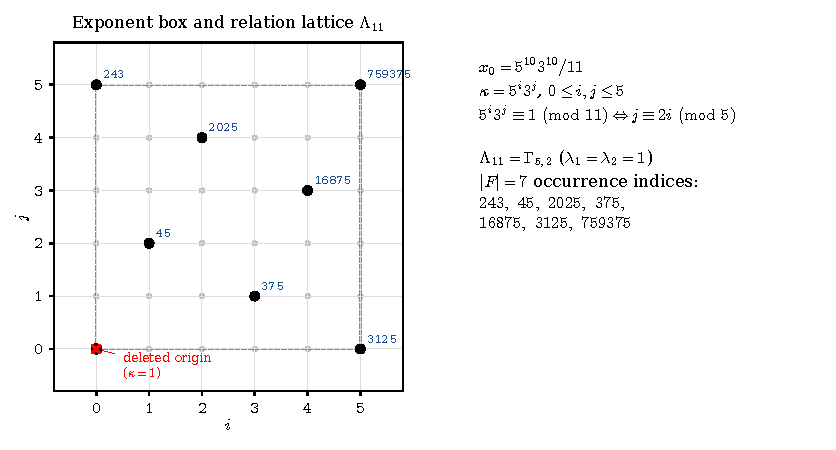
\includegraphics[width=\textwidth]{figures/fig01_fibre.pdf}
\caption{The actual occurrence fibre of $x_0=5^{10}3^{10}/11$ in prime-exponent coordinates $(i,j)$ for $5^i3^j$. Left: the box $[0,5]^2$, the lattice $\Lambda_{11}=\Gamma_{5,2}$ (black points; grey points are other integer points of the box), the deleted origin $\kappa=1$, and the occurrence indices $\kappa=5^i3^j$ at each point. Right: the defining congruence and the seven occurrence indices.}\label{fig:fibre}
\par\smallskip\noindent\figdesc{Seven black points at $(0,5),(1,2),(2,4),(3,1),(4,3),(5,0),(5,5)$ in the square $[0,5]^2$ with grey points at the remaining integer points; the origin is marked in red as deleted. Each black point carries its index $\kappa$ ($243$, $45$, $2025$, $375$, $16875$, $3125$, $759375$). The right panel states $5^i3^j\equiv1\pmod{11}\iff j\equiv2i\pmod5$.}
\end{figure}

%% -------------------------------------------------------------------
\section{Graver-cell geometry: definitions and elementary structure}\label{sec:cells}

From now on $d\ge2$ is an integer, $s\in\{1,\dots,d-1\}$ is a representative of a unit modulo $d$, $t\in\{1,\dots,d-1\}$ is the representative of $s^{-1}$, and
\[
  \Gamma=\Gamma_{d,s}=\{(i,j)\in\Z^2:\ j\equiv si\pmod d\}.
\]
Since $\Gamma$ is the kernel of the surjection $(i,j)\mapsto j-si\bmod d$, it is a sublattice of index $d$.

\begin{lemma}[Determinants]\label{lem:det}
For $g,h\in\Gamma$, $\cross(g,h)\equiv0\pmod d$.
\end{lemma}
\begin{proof}
Modulo $d$, $g_1h_2-g_2h_1\equiv g_1(sh_1)-(sg_1)h_1=0$.
\end{proof}

\subsection{Conformal order and Graver vectors}

\begin{definition}[Conformal order, Graver vectors]\label{def:conformal}
For $h,g\in\Z^2$ write $h\conf g$ if $h_ig_i\ge0$ and $|h_i|\le|g_i|$ for $i=1,2$. A nonzero $g\in\Gamma$ is a \emph{Graver vector} of $\Gamma$ if the only $h\in\Gamma$ with $h\conf g$ are $h=0$ and $h=g$. The set of Graver vectors is the \emph{Graver basis} $\mathcal G(\Gamma)$.
\end{definition}

The relation $\conf$ is a partial order on $\Z^2$ (reflexive, transitive, antisymmetric), and $\mathcal G(\Gamma)$ is the set of its minimal elements in $\Gamma\setminus\{0\}$. The Graver basis is symmetric: $g\in\mathcal G\iff-g\in\mathcal G$. For general lattices $\mathcal G$ is finite and contains every circuit; for $\Gamma_{d,s}$ we have the following explicit bound.

\begin{lemma}[Size of Graver vectors]\label{lem:graver-size}
Every Graver vector $g$ of $\Gamma$ satisfies $|g_1|\le d$ and $|g_2|\le d$. If $|g_1|=d$ or $|g_2|=d$ then $g\in\{\pm(d,0),\pm(0,d)\}$.
\end{lemma}
\begin{proof}
$(\pm d,0)$ and $(0,\pm d)$ lie in $\Gamma$ since $d\equiv0$. If $|g_1|\ge d$ then $h=(\mathrm{sgn}(g_1)d,0)\conf g$, $h\in\Gamma$, so by minimality $g=h$. If $|g_1|<d$ and $|g_2|\ge d$, symmetrically $g=(0,\pm d)$.
\end{proof}

\begin{lemma}[Standard Graver vectors]\label{lem:std-graver}
The following vectors are Graver vectors of $\Gamma_{d,s}$ (and so are their negatives):
\[
  (d,0),\quad (0,d),\quad (1,s),\quad (1,s-d),\quad (t,1),\quad (d-t,-1).
\]
\end{lemma}
\begin{proof}
$(d,0)$: if $h=(h_1,0)\conf(d,0)$ and $h\in\Gamma$, then $0\equiv sh_1$ forces $d\mid h_1$ because $s$ is a unit, so $h_1\in\{0,d\}$. The same for $(0,d)$ with the unit $s^{-1}$.

For the other four, let $g\in\Gamma$ have $|g_1|=1$ and $|g_2|<d$ (these are $(1,s)$ and $(1,s-d)$; their second coordinates satisfy $|s|,|s-d|<d$). If $h\in\Gamma$ with $h\conf g$, then $h_1\in\{0,g_1\}$. If $h_1=0$, then $d\mid h_2$ and $|h_2|\le|g_2|<d$, so $h=0$. If $h_1=g_1$, then $h_2\equiv sg_1\equiv g_2\pmod d$, $h_2$ has the sign of $g_2$ (or is zero) and $|h_2|\le|g_2|<d$; two integers congruent modulo $d$ of the same weak sign with absolute values below $d$ are equal, so $h=g$. The vectors $(t,1)$ and $(d-t,-1)$ are handled in the same way with the roles of the coordinates exchanged, using $t\equiv s^{-1}$: for $h\conf g$ with $|g_2|=1$, either $h_2=0$ and $d\mid h_1$ with $|h_1|\le|g_1|<d$, or $h_2=g_2$ and $h_1\equiv tg_2\equiv g_1\pmod d$ (indeed $sh_1\equiv g_2$ gives $h_1\equiv tg_2$, and $g_1\equiv tg_2$ for $g=(t,1)$ and $g=(d-t,-1)$).
\end{proof}

Lemma~\ref{lem:std-graver} proves the minimality of these six vectors without any box-dependent enumeration. It is the statement that supplies the Graver property of the generators $(1,-a)$ and $(c,-1)$, $a=d-s$, $c=d-t$, used for the bottom and left end cells in Section~\ref{sec:cellfamily}.

\subsection{Cells, the punctured fibre, and the realized union}

\begin{definition}[Punctured fibre and hull]\label{def:fibre}
For an integer box $Q=(Q_1,Q_2)$ with $Q_1,Q_2\ge0$ put
\[
  F_Q=F_{d,s,Q}=\bigl(\Gamma\cap[0,Q_1]\times[0,Q_2]\bigr)\setminus\{0\},\qquad H_Q=\conv(F_Q).
\]
\end{definition}

\begin{definition}[Admissible cells and the realized union]\label{def:cells}
Fix $Q$. An \emph{admissible parallelogram} is a set
\[
  P(w;g,h)=\conv\{w,\ w+g,\ w+h,\ w+g+h\}
  =\{w+\theta g+\eta h:\ \theta,\eta\in[0,1]\},
\]
where $g,h$ are linearly independent Graver vectors of $\Gamma$ and all four points $w,w+g,w+h,w+g+h$ lie in $F_Q$. An \emph{admissible segment} is $[p,p+g]$ with $g$ a Graver vector and $p,p+g\in F_Q$. An \emph{admissible point} is a point of $F_Q$. The \emph{realized union} $U_Q=U_{d,s,Q}$ is the union of all admissible parallelograms, admissible segments and admissible points.
\end{definition}

Every edge of an admissible parallelogram is an admissible segment, so the segments and points are needed only for boundary pieces and isolated points of $U_Q$ that are not contained in any parallelogram. Note that the same geometric parallelogram has several descriptions $P(w;g,h)$ (for example $P(w;g,h)=P(w+g;-g,h)$); we regard $P(w;g,h)$ as a subset of the plane, not as a triple.

\begin{figure}[ht]
\centering
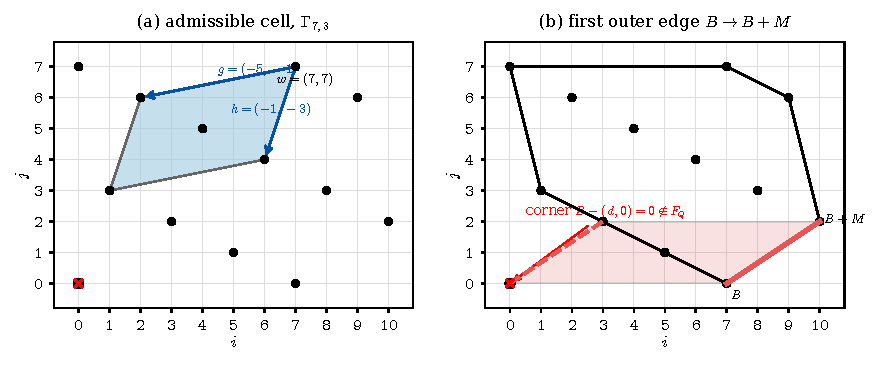
\includegraphics[width=\textwidth]{figures/fig02_cell.pdf}
\caption{(a) An admissible parallelogram $P(w;g,h)$ in $\Gamma_{7,3}$ with its two Graver generators $g,h$ and base point $w$ (the cell shown is the largest cell with corners in $F_{(7,7)}$). (b) The role of the deleted origin: the translate of the first outer edge $B\to B+M$ by $(-d,0)$ has the corner $B-(d,0)=0$, which is not in $F_Q$; this is why the first outer edge needs a separate cell (Section~\ref{sec:cellfamily}). Here $d=7$, $s=3$, $Q=(10,7)$.}\label{fig:cell}
\par\smallskip\noindent\figdesc{Left: grid of the box $[0,10]\times[0,7]$ with the lattice points of $\Gamma_{7,3}$ and one shaded parallelogram with two arrows labelled by its generators. Right: the same box, the convex hull of the points, the first edge leaving $B=(7,0)$ to the right drawn thick, and its translate by $(-7,0)$ drawn dashed with a red arrow to the origin, marked ``$B-(d,0)=0\notin F_Q$''.}
\end{figure}

\subsection{Elementary properties}

\begin{proposition}[Elementary properties]\label{prop:elem}
For every $Q\ge0$:
\begin{enumerate}
\item (\emph{Finiteness.}) There are finitely many admissible parallelograms, segments and points.
\item (\emph{Closedness.}) $U_Q$ is compact.
\item (\emph{Hull inclusion.}) $F_Q\subseteq U_Q\subseteq H_Q$.
\item (\emph{Monotonicity.}) If $Q\le Q'$ componentwise then every admissible cell for $Q$ is admissible for $Q'$ and $U_Q\subseteq U_{Q'}$.
\item (\emph{Transposition.}) Let $\tau(i,j)=(j,i)$. Then $\tau(\Gamma_{d,s})=\Gamma_{d,t}$ with $t\equiv s^{-1}$, $\tau$ preserves the conformal order, $\tau(F_{d,s,Q})=F_{d,t,(Q_2,Q_1)}$ and $\tau(U_{d,s,Q})=U_{d,t,(Q_2,Q_1)}$.
\item (\emph{Symmetry.}) The Graver basis is invariant under $g\mapsto-g$; $U_Q$ is unchanged if each cell $P(w;g,h)$ is described using $(-g,h)$ or $(g,-h)$ from the opposite corner.
\end{enumerate}
\end{proposition}
\begin{proof}
(1) Every cell is determined by its corner(s), which are points of the finite set $F_Q$ (the generators are differences of corners). (2) $U_Q$ is a finite union of compact convex sets. (3) $F_Q\subseteq U_Q$ by admissible points; each cell has its vertices in $F_Q\subseteq H_Q$, and $H_Q$ is convex, so $U_Q\subseteq H_Q$. (4) $F_Q\subseteq F_{Q'}$ and the Graver property is a property of $\Gamma$ only, not of $Q$. (5) $j\equiv si\iff i\equiv tj$; the map $\tau$ is a coordinate permutation, so it preserves $\conf$ and sends the box $[0,Q_1]\times[0,Q_2]$ to $[0,Q_2]\times[0,Q_1]$ and parallelograms to parallelograms. (6) Clear from $P(w;g,h)=P(w+g;-g,h)$.
\end{proof}

\begin{remark}
Items (1)--(4) are used silently throughout; (5) is the reason that proofs in Parts~II and III need to be carried out only for one of two symmetric configurations.
\end{remark}

\subsection{The abstract complex, the realized union, and an embedded subdivision}\label{sec:kabs}

The construction above admits three different mathematical readings which must not be confused.

\begin{definition}[$K_{\mathrm{abs}}$, $U_Q$, $K_{\mathrm{emb}}$]\label{def:kabs}
\begin{enumerate}
\item The \emph{abstract complex} $K_{\mathrm{abs}}(Q)$ is the finite regular cell complex whose vertices are the points of $F_Q$, whose edges are the admissible segments of dimension one, and whose $2$-cells are the distinct admissible parallelograms (as subsets of the plane), each attached along its four boundary edges. As a topological space it is the quotient of the disjoint union of its closed cells under the identification of shared faces by their vertex sets.
\item The \emph{realized union} is the subset $U_Q\subseteq\R^2$ of Definition~\ref{def:cells}. There is a natural continuous surjection $\pi:|K_{\mathrm{abs}}(Q)|\to U_Q$ which sends each cell affinely onto its geometric image.
\item An \emph{embedded subdivision} $K_{\mathrm{emb}}(Q)$ is any finite polyhedral complex in $\R^2$ with $|K_{\mathrm{emb}}|=U_Q$ in which every admissible cell is a union of cells; for instance the arrangement of all lines through all edges of cells, restricted to $U_Q$. It exists because $U_Q$ is a finite union of convex polygons, segments and points.
\end{enumerate}
\end{definition}

The map $\pi$ is a homeomorphism if and only if the relative interiors of distinct cells are pairwise disjoint and any two cells meet in a common face (compare the face-closed embeddedness criterion in the GEO-I record, listed in Appendix~\ref{app:registry} as context only). In general neither is true: distinct admissible parallelograms can overlap in a region, so that $\pi$ is not injective, and $|K_{\mathrm{abs}}|$ and $U_Q$ need not even have the same Betti numbers. The set $U_Q$ is a compact polyhedron regardless, and its topology is determined by $K_{\mathrm{emb}}$.

\begin{example}[Overlapping cells]\label{ex:overlap}
For $(d,s,Q)=(5,2,(5,5))$ there are exactly four distinct admissible parallelograms. With $v_1=(1,-3)$, $v_2=(2,-1)$, $f=(1,2)$,
\[
\begin{aligned}
C_1&=P\bigl((0,5);v_1,v_2\bigr), &C_2&=P\bigl((1,2);f,v_2\bigr),\\
C_3&=P\bigl((1,2);f,(3,1)\bigr), &C_4&=P\bigl((2,4);v_1,v_2\bigr).
\end{aligned}
\]
Each has area $5=d$, so the cells have total area $20$. The realized union $U_Q$ has area $17.5-5=12.5$ (Theorem~\ref{thm:exceptional}), so the total area of the cells exceeds the area of their union by $7.5$. The statements proved in this paper concern the set $U_Q$ and not $K_{\mathrm{abs}}$.
\end{example}

\begin{remark}[Modelling choice]\label{rem:modelling}
The attachment rule of Definition~\ref{def:cells} is a modelling decision. Arithmetic gives the lattice points (Theorem~\ref{thm:occ}) and the relations between them (Section~\ref{sec:arith-meaning}) exactly. Which one-dimensional and two-dimensional pieces to attach is a choice of geometry, made so that each attached piece is spanned by primitive relations among occurrence coordinates. A different attachment rule could yield different topology; it would not alter any statement about lattice points. Consequently, ``the topology of the occurrence fibre'' in this paper always means the topology of $U_Q$, as in the abstract.
\end{remark}

\begin{remark}[Convexity versus embedding]
Theorem~\ref{thm:universal} states $U_Q=H_Q$. It does not say that the admissible cells form a face-to-face tiling of $H_Q$, and in general they do not (Example~\ref{ex:overlap}, and the figures in Part~III in which cells of different colours overlap). The convex hull $H_Q$ itself is contractible, so a statement $U_Q=H_Q$ determines the topology of $U_Q$ without any information about $K_{\mathrm{abs}}$.
\end{remark}

%% ===================================================================
%% PART II
%% ===================================================================
\part{Exceptional topology and hole filling}

\section{The exceptional occurrence square}\label{sec:exceptional}

Let $d\ge2$, $s$ a unit modulo $d$ with representative $1\le s\le d-1$, $t\equiv s^{-1}$ with $1\le t\le d-1$, and put $a=d-s$, $c=d-t$ (these are the integers $a_s$, $c_t$ of Table~\ref{tab:notation}; the shorthand is used from here on). Write
\[
  Q_0=(d,d),\qquad H_0=H_{Q_0},\qquad U_0=U_{Q_0}.
\]
The box $Q_0$ is the smallest box in which both axis relations $(d,0)$ and $(0,d)$ are visible, and it is the box in which the realized union fails to be convex. This section describes its fibre and proves that two explicit triangles cannot be covered.

\subsection{The exceptional fibre}

Define
\[
  A=(0,d),\qquad B=(d,0),\qquad C_0=(d,d),\qquad P_i=(i,\ si\bmod d)\quad(1\le i\le d-1),
\]
where $si\bmod d\in\{1,\dots,d-1\}$ is the least positive residue (it is nonzero since $s$ is a unit and $d\nmid i$).

\begin{lemma}[The exceptional fibre]\label{lem:exc-fibre}
$F_{Q_0}=\{A,B,C_0,P_1,\dots,P_{d-1}\}$, a set of $d+2$ points.
\end{lemma}
\begin{proof}
Let $(i,j)\in\Gamma\cap[0,d]^2$, $(i,j)\ne0$. If $i=0$ then $d\mid j$, so $j=d$ and the point is $A$. If $i=d$ then $d\mid j$, so $j\in\{0,d\}$: the points $B$ and $C_0$. If $1\le i\le d-1$ then $j\equiv si\not\equiv0$ so $1\le j\le d-1$ and $j=si\bmod d$.
\end{proof}

The residue points satisfy
\begin{equation}\label{eq:special-P}
  P_{d-t}=(d-t,\ d-1)=(c,d-1),\qquad P_{d-1}=(d-1,\ d-s)=(d-1,a),
\end{equation}
because $s(d-t)\equiv-st\equiv-1$ and $s(d-1)\equiv-s$. Also $P_t=(t,1)$ and $P_1=(1,s)$.

\subsection{The two triangles}

\begin{definition}[The exceptional triangles]\label{def:T}
\[
  T_1=\conv(A,\ P_{d-t},\ C_0),\qquad T_2=\conv(B,\ P_{d-1},\ C_0).
\]
\end{definition}

The edges of $T_1$ are $\overrightarrow{AP_{d-t}}=(c,-1)=(d-t,-1)$, $\overrightarrow{P_{d-t}C_0}=(t,1)$ and $\overrightarrow{AC_0}=(d,0)$. By Lemma~\ref{lem:std-graver} all three are Graver vectors, so the three edges of $T_1$ are admissible segments and
\begin{equation}\label{eq:dT1}
  \partial T_1\subseteq U_0.
\end{equation}
For $T_2$ the edges are $\overrightarrow{BP_{d-1}}=(-1,a)$, $\overrightarrow{P_{d-1}C_0}=(1,s)$ and $\overrightarrow{BC_0}=(0,d)$, again Graver, so $\partial T_2\subseteq U_0$.

\begin{lemma}[Transposition exchanges $T_1$ and $T_2$]\label{lem:T-transpose}
Let $\tau(i,j)=(j,i)$. Then $\tau(T_1(d,s))=T_2(d,t)$ and $\tau(T_2(d,s))=T_1(d,t)$. In particular any statement proved for $T_1$ in all $(d,s)$ holds for $T_2$ in all $(d,s)$.
\end{lemma}
\begin{proof}
$\tau$ maps $A\mapsto B$, $C_0\mapsto C_0$ and $P_{d-t}=(d-t,d-1)\mapsto(d-1,d-t)$. In $\Gamma_{d,t}$ (whose inverse unit is $s$) the point $P_{d-1}$ is $(d-1,\,t(d-1)\bmod d)=(d-1,d-t)$. Hence $\tau(T_1(d,s))=\conv(B,P'_{d-1},C_0)=T_2(d,t)$. The second identity follows by applying $\tau$ again.
\end{proof}

\begin{lemma}[Area and disjointness]\label{lem:T-disjoint}
$T_1$ and $T_2$ have area $d/2$ each, and $\interior T_1\cap\interior T_2=\varnothing$.
\end{lemma}
\begin{proof}
$\mathrm{area}(T_1)=\tfrac12|\cross((c,-1),(d,0))|=\tfrac12 d$, and $T_2$ is its transposed image for $(d,t)$.

Let $X=x-d$, $Y=y-d$ be coordinates centred at $C_0$. Then $T_1$ lies in the cone $\{Y\le0,\ X\le tY\}$ spanned by $A-C_0=(-d,0)$ and $P_{d-t}-C_0=(-t,-1)$, and $T_2$ lies in the cone $\{X\le0,\ Y\le sX\}$ spanned by $B-C_0=(0,-d)$ and $P_{d-1}-C_0=(-1,-s)$. A common interior point would satisfy $Y<0$, $X<tY$ and $X<0$, $Y<sX$; then $X<tY<tsX$, that is $(1-st)X<0$. But $X<0$ and $st\ge1$ give $(1-st)X\ge0$, a contradiction.
\end{proof}

The directions $(c,-1)$ and $(t,1)$ are the two primitive lattice directions which, with $(d,0)$, bound the triangle $T_1$. Since $\{u,v\}=\{(c,-1),(d,0)\}$ is a basis of $\Gamma$ (its determinant is $d$, the index), the triangle $T_1=\conv(A,A+u,A+v)$ is half of a fundamental parallelogram of $\Gamma$: it is unimodular with respect to $\Gamma$ and contains no lattice point other than its three vertices. This is the sense in which it is an arithmetic object and not a drawing artefact.

\begin{figure}[ht]
\centering
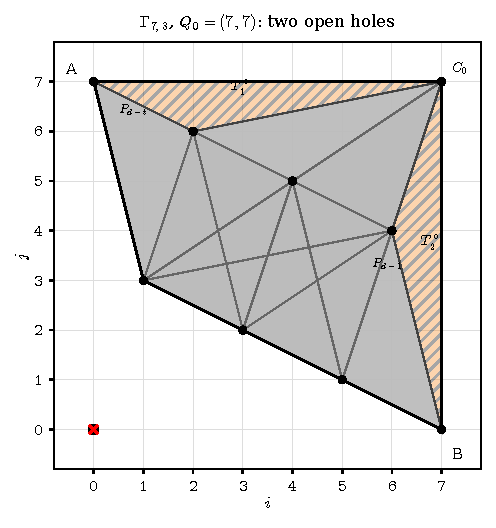
\includegraphics[width=.62\textwidth]{figures/fig03_two_holes.pdf}
\caption{The realized union in the exceptional box, $d=7$, $s=3$ ($t=5$), $Q_0=(7,7)$. Shaded: all admissible parallelograms. The segments are drawn in grey. The two white triangles $T_1=\conv(A,P_{d-t},C_0)$ and $T_2=\conv(B,P_{d-1},C_0)$ are not covered; their boundaries are.}\label{fig:two-holes}
\par\smallskip\noindent\figdesc{A square $[0,7]^2$ with the convex hull of the fibre outlined, many overlapping pale parallelograms covering most of it, and two white triangles near the top and right sides, both having the upper right corner $C_0=(7,7)$ as a vertex. The vertices $A$, $B$, $C_0$, $P_{d-t}$ and $P_{d-1}$ are labelled.}
\end{figure}

\subsection{The triangle interiors are not covered}

\begin{lemma}[Affine coordinates adapted to $T_1$]\label{lem:eta-xi}
Put $u=(c,-1)$ and $v=(d,0)$. For $p\in\Gamma$ write $p-A=\eta u+\xi v$. Then $\eta=d-p_y$ and $\xi=(p_x-\eta c)/d$ are integers. In the coordinates $(\eta,\xi)$, $A=(0,0)$, $P_{d-t}=(1,0)$, $C_0=(0,1)$ and $T_1$ is the triangle with vertices $(0,0),(1,0),(0,1)$.
\end{lemma}
\begin{proof}
The two equations $p_y-d=-\eta$ and $p_x=\eta c+\xi d$ give the stated formulas. Modulo $d$: $\eta c=(d-p_y)(d-t)\equiv tp_y\equiv tsp_x\equiv p_x$, so $d\mid p_x-\eta c$. The three vertex coordinates are immediate from $P_{d-t}-A=(c,-1)=u$ and $C_0-A=(d,0)=v$.
\end{proof}

\begin{proposition}[Exclusion of the open triangles]\label{prop:hole-exclusion}
For every $d\ge2$ and every unit $s$: $\partial T_1\subseteq U_0$ and $\interior T_1\cap U_0=\varnothing$. The same holds for $T_2$.
\end{proposition}
\begin{proof}
The inclusion $\partial T_1\subseteq U_0$ is \eqref{eq:dT1}. By Lemma~\ref{lem:T-transpose} it suffices to prove the exclusion for $T_1$. Work in the coordinates of Lemma~\ref{lem:eta-xi}. Then $\interior T_1=\{\eta>0,\xi>0,\eta+\xi<1\}$; every point of $F_{Q_0}$ has integer coordinates $(\eta,\xi)$ with $\eta=d-p_y\ge0$, so no point of $F_{Q_0}$ lies in $\interior T_1$ (``Step 0'').

\emph{Step 1: no admissible segment meets $\interior T_1$.} Let $[p,q]$ be an admissible segment with $q-p$ Graver, $p,q\in F_{Q_0}$, and suppose it contains a point of $\interior T_1$. Along the segment $\eta$ is affine and takes a value in $(0,1)$ at some point, while its endpoint values are integers $\ge0$. Hence one endpoint has $\eta=0$ and the other $\eta\ge1$. The points of $F_{Q_0}$ with $\eta=0$ (that is $p_y=d$) are $A=(0,0)_{\eta\xi}$ and $C_0=(0,1)_{\eta\xi}$ by Lemma~\ref{lem:exc-fibre}.

\emph{(a) The endpoint with $\eta=0$ is $A$.} Let $q=(\eta_q,\xi_q)$, $\eta_q\ge1$. The segment from $(0,0)$ to $q$ meets $\interior T_1$ only if some positive multiple $\theta q$ has $\theta\xi_q>0$ and $\theta(\eta_q+\xi_q)<1$; thus $\xi_q\ge1$. Then
\[
  q-A=\eta_qu+\xi_qv=(\eta_qc+\xi_qd,\ -\eta_q),
\]
and $u=(c,-1)$ satisfies $u\conf q-A$ (same signs, $c\le\eta_qc+\xi_qd$, $1\le\eta_q$), $u\in\Gamma$, $u\ne q-A$ because $\xi_q\ge1$. This contradicts the Graver property of $q-A$.

\emph{(b) The endpoint with $\eta=0$ is $C_0=(0,1)_{\eta\xi}$.} Let $q=(\eta_q,\xi_q)$ with $\eta_q\ge1$. A point $C_0+\theta(q-C_0)=(\theta\eta_q,\ 1+\theta(\xi_q-1))$, $0<\theta<1$, lies in $\interior T_1$ only if $\eta+\xi<1$, that is $\theta(\eta_q+\xi_q-1)<0$, so $\eta_q+\xi_q\le0$ as these are integers. Then $\xi_q\le-\eta_q$ and
\[
  q_x=\eta_qc+\xi_qd\le\eta_q(c-d)=-\eta_qt<0,
\]
which is impossible for a point of the box.

\emph{Step 2: no admissible parallelogram meets $\interior T_1$.} Let $P$ be an admissible parallelogram meeting $\interior T_1$. No vertex of $P$ is in $\interior T_1$ (Step 0), and no edge of $P$ meets $\interior T_1$ (Step 1, since edges are admissible segments). The set $\interior T_1$ is connected and disjoint from $\partial P$, so the nonempty set $\interior T_1\cap P$ is open and closed in $\interior T_1$, hence $\interior T_1\subseteq\interior P$. Then $A,C_0\in P$ and the segment $AC_0\subset P$. Since $P\subseteq[0,d]^2$ lies below the line $y=d$, $P\cap\{y=d\}$ is a face of $P$ containing the segment $AC_0$ of length $d$, so it is an edge of $P$ lying in $[0,d]\times\{d\}$ and containing $AC_0$, hence equal to $AC_0$. This edge is a Graver generator up to sign, namely $\pm(d,0)$. The other generator $h$ is independent and points downward ($h_y<0$) since $P\subseteq\{y\le d\}$. The other two corners are $A+h$ and $C_0+h$, which must lie in $[0,d]^2$, so $0\le h_x$ and $d+h_x\le d$, hence $h_x=0$ and $h=(0,-m)$ with $d\mid m$ (lattice condition) and $(0,-m)$ Graver, which forces $m=d$ by Lemma~\ref{lem:graver-size}. Then $A+h=(0,0)$, which is not in $F_{Q_0}$. Contradiction.

\emph{Conclusion.} $U_0$ is the union of admissible points, segments and parallelograms; none meets $\interior T_1$.
\end{proof}

\begin{remark}\label{rem:holes-lowerbound}
Proposition~\ref{prop:hole-exclusion} gives the lower bound $\beta_1(U_0)\ge 2$ in all classes where the two open triangles are bounded components of the complement (Section~\ref{sec:topology}). It does not, by itself, say that nothing else is missing from $H_0$; that is the content of the next section.
\end{remark}

%% -------------------------------------------------------------------
\section{Exact exceptional complement in nonspecial modular classes}\label{sec:nonspecial}

\begin{definition}[Nonspecial class]
The class $(d,s)$ is \emph{nonspecial} if $d\ge5$ and $2\le s\le d-2$ with $\gcd(s,d)=1$. Equivalently $a=d-s\ge2$, $c=d-t\ge2$, $s\ge2$, $t\ge2$. The classes $s\equiv\pm1$ are \emph{special}. For $d\in\{2,3,4,6\}$ every unit is special.
\end{definition}

\begin{theorem}[Nonspecial exceptional complement]\label{thm:exceptional}
If $d\ge5$, $2\le s\le d-2$ and $\gcd(s,d)=1$, then
\[
  \boxed{\,H_0\setminus U_0=\interior T_1\ \sqcup\ \interior T_2.\,}
\]
In particular $U_0=H_0\setminus(\interior T_1\cup\interior T_2)$, so $U_0$ is the closed polygon $H_0$ with two disjoint open triangles of area $d/2$ removed.
\end{theorem}

The proof has four ingredients: the lower-left chain of $H_0$ and its Graver steps (Lemma~\ref{lem:chain0}), a zonogon built from these steps and tiled by admissible parallelograms (Lemma~\ref{lem:zonogon}), one additional admissible cell $K$ (Lemma~\ref{lem:K}), and a covering argument (Lemma~\ref{lem:cover0}). The inclusion $\supseteq$ in the theorem is Proposition~\ref{prop:hole-exclusion}.

\subsection{The lower-left chain}

The boundary of $H_0$ consists of the segment $AC_0$ on $y=d$, the segment $C_0B$ on $x=d$ (both are in $H_0$ since $A,B,C_0\in F_{Q_0}$), and a convex arc from $A$ to $B$ on the lower-left, which we call the \emph{lower-left chain}.

\begin{lemma}[Lower-left chain]\label{lem:chain0}
Let $A=c_0,c_1,\dots,c_n=B$ be all lattice points of $\Gamma$ lying on the lower-left chain, in order along it, including collinear ones, and put $v_i=c_i-c_{i-1}=(a_i,-b_i)$. Then:
\begin{enumerate}
\item $a_i>0$ and $b_i>0$ for all $i$, and $b_1/a_1\ge b_2/a_2\ge\dots\ge b_n/a_n$;
\item every $v_i$ is a Graver vector;
\item $v_1=(1,s-d)=(1,-a)$ and $v_n=(d-t,-1)=(c,-1)$; in particular $n\ge2$ in a nonspecial class;
\item $\sum a_i=d$ and $\sum b_i=d$.
\end{enumerate}
\end{lemma}
\begin{proof}
(1) The chain is the graph of a convex function $f$ on $[0,d]$ with $f(0)=d$, $f(d)=0$ and $f\ge0$ on $[0,d]$ (the hull lies in the box). A convex function with $f(d)=0=\min f$ is nonincreasing, and it is strictly decreasing, since $f=0$ on an interval $[x_0,d]$, $x_0<d$, would put a lattice point $(i,0)$ with $0<i<d$ on the chain, but $(i,0)\in\Gamma$ forces $d\mid i$. Convexity gives nonincreasing $b_i/a_i$ (the slopes $-b_i/a_i$ are nondecreasing).

(2) Each pair $c_{i-1},c_i$ is a pair of consecutive boundary lattice points of $H_{Q_0}$ with $Q_0\ge(d,d)$; this is the boundary lemma (Lemma~\ref{lem:reflection}, Section~\ref{sec:reflection}, whose proof does not depend on the present section).

(3) Let $q=(q_x,q_y)\in F_{Q_0}$ with $q_x<d$, and write $B-q=(a',-b')$ with $a'=d-q_x\ge1$, $b'=q_y\ge0$. The last edge of the chain ends at $B$ and is the supporting line of $H_0$ at $B$ on the lower-left side, whose slope $b_n/a_n$ minimizes $b'/a'$ over all such $q$ (all of $H_0$ lies on or above this line). We claim that the minimum is attained at $q=(t,1)\in F_{Q_0}$, where $b'/a'=1/c$. Let $q\notin\{A\}$ (for $A$, $b'/a'=1\ge1/c$). Then $q=(d-a',b')$ with $1\le a'\le d-1$, $1\le b'\le d-1$, and the lattice condition $b'\equiv s(d-a')\equiv-sa'$ gives, after multiplying by $t$, $a'+tb'\equiv0\pmod d$. Write $tb'=md+r$ with $0\le r<d$. Since $t<d$ we have $m\le b'-1$. As $a'\ge1$ and $a'\equiv-r$, $r\neq0$ and $a'=d-r$. Then
\[
  b'c-a'=b'd-b't-d+r=(b'-m-1)d\ge0.
\]
Hence $a'\le b'c$, that is $b'/a'\ge1/c$, with equality exactly when $a'=b'c$. Points of equality lie on the line through $B$ with direction $(c,-1)$; the lattice point of this line nearest to $B$ is $(t,1)$, since $a'=b'c\ge c$ with equality only for $b'=1$. So $(t,1)$ is the lattice point preceding $B$ on the chain and $v_n=B-(t,1)=(c,-1)$. Transposition (Proposition~\ref{prop:elem}(5)) turns this into the statement for the first step: in $\Gamma_{d,t}$ the last step into $B$ is $(d-s,-1)$, and transposing and reversing gives the first step $v_1=(1,-(d-s))=(1,s-d)$ in $\Gamma_{d,s}$. Finally $(1,-a)=(c,-1)$ would force $a=c=1$, that is $s=t=d-1$, a special class; hence $v_1\ne v_n$ and $n\ge2$ in a nonspecial class.

(4) $c_0=A$ and $c_n=B$.
\end{proof}

\subsection{The zonogon}

Let $Z=A+\sum_{i=1}^n[0,v_i]$ be the zonogon generated by the chain steps. Its lower-left boundary is the chain (steps in the order $v_1,\dots,v_n$, steep to shallow) and its upper-right boundary is the chain with steps in the reverse order $v_n,\dots,v_1$.

\begin{lemma}[Zonogon cover]\label{lem:zonogon}
Let $d\ge5$ be nonspecial. There is a finite family of admissible parallelograms with vertex sets in $\{A+\sum_{i\in S}v_i:S\subseteq\{1,\dots,n\}\}$ whose union is $Z$. In particular $Z\subseteq U_0$.
\end{lemma}
\begin{proof}
\emph{All subset sums are admissible corners.} For $S\subseteq\{1,\dots,n\}$ the point $z_S=A+\sum_{i\in S}v_i$ lies in $\Gamma$ (a sum of lattice vectors), and its coordinates are $x=\sum_{i\in S}a_i\in[0,d]$, $y=d-\sum_{i\in S}b_i\in[0,d]$, by Lemma~\ref{lem:chain0}(4). If $z_S=0$ then $x=0$ forces $S=\varnothing$, giving $z_S=A\ne0$. So $z_S\in F_{Q_0}$ for every $S$.

\emph{Sweeping construction.} Put $Z_k=A+\sum_{i\le k}[0,v_i]$. We show by induction on $k$ that $Z_k$ is covered by admissible parallelograms with corners among the subset sums. For $k=1$ the set $Z_1$ is the Graver segment $[A,A+v_1]$, which is admissible. Let $k\ge2$ and assume the claim for $Z_{k-1}$. Put $\psi(z)=\cross(v_k,z)=a_kz_y+b_kz_x$. For $i<k$ the slope ordering gives
\[
  \psi(v_i)=b_ka_i-a_kb_i\le0,\quad\text{with equality exactly when }v_i\parallel v_k.
\]
Hence over $Z_{k-1}$ the functional $\psi$ has its maximum at $A$ and its minimum at $A+\sum_{i<k}v_i$, and the boundary of $Z_{k-1}$ splits at these two points into the lower-left chain, with edges $v_1,\dots,v_{k-1}$ in this order, and the upper-right chain, with edges $v_{k-1},\dots,v_1$ in this order from $A$. An edge of direction $v_i$ on the upper-right chain has outward normal $n=(b_i,a_i)$ and $n\cdot v_k=-\psi(v_i)\ge0$; on the lower-left chain the outward normal $(-b_i,-a_i)$ has $n\cdot v_k=\psi(v_i)\le0$.

For a convex polygon $P$ and a vector $v$ one has $P+[0,v]=P\cup\bigcup_e\,(e+[0,v])$, the union over the edges $e$ whose outward normal $n$ satisfies $n\cdot v>0$. (If $z\in P$, $0<\theta\le1$ and $z+\theta v\notin P$, the ray from $z$ in direction $v$ leaves $P$ at a point $z'$ of such an edge and $z+\theta v=z'+\lambda v$ with $0<\lambda\le1$; the converse inclusion is clear.) Here the relevant edges are the edges of the upper-right chain not parallel to $v_k$. Each such edge, $e=[w,w+v_i]$ with $w$ a subset sum, sweeps the parallelogram $e+[0,v_k]=P(w;v_i,v_k)$, whose four corners are subset sums, whose generators $v_i,v_k$ are Graver (Lemma~\ref{lem:chain0}(2)) and independent. Edges parallel to $v_k$ sweep nothing. So $Z_k=Z_{k-1}\cup\bigcup P(w;v_i,v_k)$ is covered by admissible parallelograms. Repeated parallel steps cause no difficulty: they produce collinear boundary edges and no new tiles.

For $k=n$ we get $Z_n=Z$.
\end{proof}

\begin{figure}[ht]
\centering
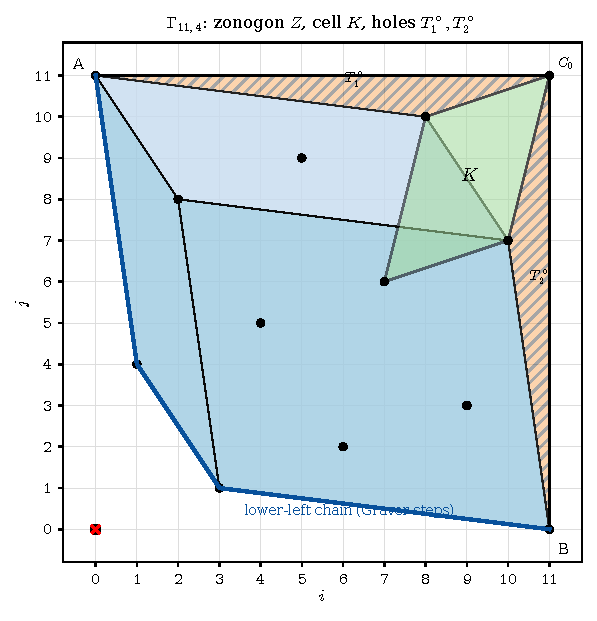
\includegraphics[width=.7\textwidth]{figures/fig04_zonogon.pdf}
\caption{$d=11$, $s=4$ ($t=3$): the zonogon $Z$ (blue tiles, alternating shades) generated by the Graver steps of the lower-left chain (thick blue), the extra cell $K$ (orange) and the two open triangles $T_1^\circ,T_2^\circ$ (white). Together they cover $H_0$.}\label{fig:zonogon}
\par\smallskip\noindent\figdesc{A square $[0,11]^2$ with the lower-left chain from $A=(0,11)$ to $B=(11,0)$ drawn thick; the zonogon it generates is tiled by parallelograms of two alternating blue shades; one orange parallelogram $K$ sits near the upper right corner between the zonogon's upper chain and $C_0$; two white triangles with vertex $C_0$ complete the hull.}
\end{figure}

\subsection{\texorpdfstring{The additional cell $K$}{The additional cell K}}

\begin{lemma}[The cell $K$]\label{lem:K}
For a nonspecial class put $w_K=(c-1,\ a-1)$ and
\[
  K=P\bigl(w_K;\ (1,s),\ (t,1)\bigr).
\]
Its corners are $w_K$, $L=P_{d-t}=(c,d-1)$, $R=P_{d-1}=(d-1,a)$ and $C_0$. The cell $K$ is admissible, so $K\subseteq U_0$.
\end{lemma}
\begin{proof}
$w_K+(1,s)=(c,a-1+s)=(c,d-1)=L$, $w_K+(t,1)=(c-1+t,a)=(d-1,a)=R$, and $w_K+(1,s)+(t,1)=(c+t,a+s)=(d,d)=C_0$. In a nonspecial class $c\ge2$ and $a\ge2$, so $w_K$ has positive coordinates; it lies in $\Gamma$ because $w_K=L-(1,s)$, and in the box. The four corners are in $F_{Q_0}$. The generators $(1,s)$ and $(t,1)$ are Graver (Lemma~\ref{lem:std-graver}) with $\cross((1,s),(t,1))=1-st$, which is nonzero since $s,t\ge2$ give $st\ge4$.
\end{proof}

\subsection{Covering}

\begin{lemma}[Covering of $H_0$]\label{lem:cover0}
In a nonspecial class, $H_0\subseteq Z\cup T_1\cup T_2\cup K$.
\end{lemma}
\begin{proof}
For $0\le x\le d$ the vertical slice of $H_0$ is $[f(x),g(x)]$, where $f$ is the lower-left chain, $g(x)=d$ for $0\le x<d$ (the side $AC_0$) and the slice at $x=d$ is $[0,d]$ (the side $C_0B$). The vertical slice of $Z$ is $[f(x),h(x)]$, where $h$ is the concave function whose graph is the upper-right chain of $Z$. This chain begins with the edge from $A$ to $A+v_n=L=(c,d-1)$ and ends with the edge from $R=B-v_1=(d-1,a)$ to $B$ (Lemma~
ef{lem:chain0}(3)). Let $z\in H_0\setminus Z$; then $h(z_x)<z_y\le g(z_x)$. Write $E_1=(c,d)$ and $E_2=(d,a)$; these are points of the sides $AC_0$ and $C_0B$.

\emph{Region I: $z_x\le c$.} On $[0,c]$ the function $h$ is the segment $AL$, so $z$ lies on or above $AL$ and on or below $y=d$, that is in the triangle $\conv(A,L,E_1)\subseteq T_1$.

\emph{Region II: $z_y\le a$.} The upper-right chain of $Z$ is monotone (the abscissa increases and the ordinate decreases along it), so horizontal slices of $Z$ are intervals, and on the heights $0\le y\le a$ its right end is the segment $RB$. A point $z\in H_0\setminus Z$ with $z_y\le a$ therefore lies to the right of the segment $RB$ and to the left of $x=d$: in the triangle $\conv(B,R,E_2)\subseteq T_2$.

\emph{Region III: $z_x>c$ and $z_y>a$.} Then $z\in[c,d]\times[a,d]$. We claim that $z$ lies on or above the line $LR$. If $c<z_x\le d-1$, $z$ lies above the concave chain of $Z$ from $L$ to $R$, which lies on or above the chord $LR$. If $z_x>d-1$ then $z_y>a$, and the line $LR$ has ordinate below $a$ there. Now the part of the rectangle $[c,d]\times[a,d]$ on or above the line $LR$ is the convex pentagon with vertices $L,E_1,C_0,E_2,R$, which is the union of the three triangles $\conv(C_0,L,E_1)$, $\conv(C_0,L,R)$, $\conv(C_0,R,E_2)$. The first is contained in $T_1$ (its vertices lie in $T_1$), the third in $T_2$, and the second is $\Delta=\conv(L,R,C_0)\subseteq K$ since three of the corners of the parallelogram $K$ are $L,R,C_0$ (Lemma~\ref{lem:K}).

The three regions exhaust $H_0\setminus Z$.
\end{proof}

\begin{proof}[Proof of Theorem~\ref{thm:exceptional}]
By Lemmas~\ref{lem:zonogon} and \ref{lem:K}, $Z\cup K\subseteq U_0$. By \eqref{eq:dT1}, $\partial T_i\subseteq U_0$. By Lemma~\ref{lem:cover0}, every point of $H_0\setminus U_0$ lies in $T_1\cup T_2$ and not in $\partial T_1\cup\partial T_2$; hence $H_0\setminus U_0\subseteq\interior T_1\cup\interior T_2$. Conversely $T_i\subseteq H_0$ because the vertices of $T_i$ are in $F_{Q_0}$, and $\interior T_i\cap U_0=\varnothing$ by Proposition~\ref{prop:hole-exclusion}. The two open triangles are disjoint by Lemma~\ref{lem:T-disjoint}.
\end{proof}

\begin{remark}[Both inclusions]
The theorem is an equality of sets: the inclusion $H_0\setminus U_0\subseteq\interior T_1\sqcup\interior T_2$ is the covering argument (Lemmas~\ref{lem:zonogon}--\ref{lem:cover0}), and the reverse inclusion is the exclusion argument (Proposition~\ref{prop:hole-exclusion}), which includes the treatment of the deleted origin.
\end{remark}

\begin{remark}[Modular sail]
The lower-left chain of $H_0$ is the part between $A$ and $B$ of the boundary of $\conv\bigl(\Gamma\cap\R_{\ge0}^2\setminus\{0\}\bigr)$, the Klein sail of the lattice in the quadrant (Proposition~\ref{prop:persist} below shows that every nonzero lattice point of the quadrant lies on the upper-right side of each supporting line of the chain). The chain steps in Lemma~\ref{lem:chain0} are the consecutive vectors of this sail. For the lattice $\Gamma_{d,s}$ the sail is governed by the continued fraction of $s/d$; we do not use this.
\end{remark}

\begin{remark}[The cells overlap]
The union $Z\cup K\cup T_1\cup T_2$ is a cover, not a tiling. For $(d,s)=(5,2)$ the zonogon has area $10$, $K$ has area $5$ and $T_1,T_2$ have area $2.5$ each; the hull has area $17.5$, so $K$ overlaps $Z$ in area $2.5$ (the part of $K$ below the chord $LR$ of Lemma~\ref{lem:cover0}).
\end{remark}

%% -------------------------------------------------------------------
\section{Special modular classes and exceptional configurations}\label{sec:special-classes}

The classes $s\equiv-1$ and $s\equiv+1\pmod d$ are treated separately: they have different fibres, different Graver bases and, for $s\equiv-1$, different topology. Both rely on the complete lists of Graver vectors proved in Lemma~\ref{lem:special-graver} (Section~\ref{sec:special-stab}, whose proof does not depend on the present section).

\subsection{\texorpdfstring{The class $s\equiv-1$: the fan graph}{The class s = -1: the fan graph}}

Let $s=d-1$, so $t=d-1$, $\Gamma=\{(i,j):i+j\equiv0\ (\mathrm{mod}\ d)\}$.

\begin{proposition}[The fan graph]\label{prop:special-fan}
For $s=d-1$ and $d\ge2$, $F_{Q_0}=\{E_0,\dots,E_d\}\cup\{C_0\}$ with $E_i=(i,d-i)$ (so $E_0=A$, $E_d=B$). The set $U_0$ is the union of the $d$ segments $[E_{i-1},E_i]$ and the $d+1$ spokes $[E_i,C_0]$. It is a connected planar graph with $d+2$ vertices and $2d+1$ edges, containing no two-dimensional cell, with
\[
  \beta_1(U_0)=d,\qquad\beta_2(U_0)=0.
\]
The complement $H_0\setminus U_0$ is the disjoint union of the $d$ open triangles $\interior\conv(E_{i-1},E_i,C_0)$, each of area $d/2$; $T_1$ and $T_2$ are two of them.
\end{proposition}
\begin{proof}
A point $(i,j)\in\Gamma\cap[0,d]^2\setminus\{0\}$ has $i+j\in\{d,2d\}$, giving the antidiagonal points $E_0,\dots,E_d$ and the single point $C_0=(d,d)$. By Lemma~\ref{lem:special-graver} the Graver vectors are $\pm(1,-1)$ and $\pm(k,d-k)$, $0\le k\le d$. Then $E_i-E_{i-1}=(1,-1)$ is Graver, whereas $E_j-E_i=(j-i)(1,-1)$ for $j-i\ge2$ is not (it has $(1,-1)$ conformally below it); and $C_0-E_i=(d-i,i)=(k,d-k)$ with $k=d-i$ is Graver. So the admissible segments are the stated ones (and unions of them).

No admissible parallelogram exists: the four corners of a nondegenerate parallelogram have no three collinear, but any four points of $F_{Q_0}$ contain at least three of the collinear points $E_i$.

Thus $U_0$ is the union of the antidiagonal segment $[A,B]$ (subdivided at the $E_i$) and the spokes. A spoke meets the line $x+y=d$ only at its endpoint $E_i$, because $C_0$ is off that line; spokes meet one another only at $C_0$. So $U_0$ is an embedded graph with $V=d+2$ vertices and $E=d+(d+1)=2d+1$ edges. It is connected, hence $\beta_1=E-V+1=d$. A graph has no $H_2$.

The hull $H_0=\conv(A,B,C_0)$ has area $d^2/2$. The $d$ triangles $\conv(E_{i-1},E_i,C_0)$ form a fan from $C_0$ over the subdivided side $[A,B]$, so they have disjoint interiors and their union is $H_0$; each has area $\tfrac12|\cross(E_i-E_{i-1},\,C_0-E_{i-1})|=\tfrac12|\cross((1,-1),(d-i+1,i-1))|=d/2$. Each is bounded by edges of the graph, so the interiors are the components of $H_0\setminus U_0$. For $s=t=d-1$ we have $P_{d-t}=P_1=E_1$ and $P_{d-1}=E_{d-1}$, so $T_1=\conv(A,E_1,C_0)$ and $T_2=\conv(B,E_{d-1},C_0)$ are the first and last of these triangles.
\end{proof}

\subsection{\texorpdfstring{The class $s\equiv+1$ with $d\ge3$: the exact complement}{The class s = +1 with d >= 3: the exact complement}}

\begin{remark}[Source status]\label{rem:s1-source}
The identity $\beta_1(U_0)=2$ for $s\equiv+1$, $d\ge3$ is recorded in the GEO-I releases (v005, G5-C2). The exact description of the \emph{complement} $H_0\setminus U_0$ given in Proposition~\ref{prop:special-plus} below, and its proof from the explicit cell list, were derived in the working draft preceding this manuscript (the ``v2 mathematical core'') and are not attributed to v005 as a theorem stated there. In the v005 notation the roles of $A$ and $B$ are interchanged.
\end{remark}

Let $s=1$, $t=1$, $\Gamma=\{(i,j):j\equiv i\ (\mathrm{mod}\ d)\}$, $d\ge3$. Put $D_i=(i,i)$ for $1\le i\le d$, so $D_d=C_0$. By Lemma~\ref{lem:exc-fibre}, $F_{Q_0}=\{A,B,D_1,\dots,D_d\}$, and $P_i=D_i$.

\begin{proposition}[The class $s=1$]\label{prop:special-plus}
Let $s=1$, $d\ge3$ and
\[
  W=P\bigl(A;\ (1,1-d),\ (d-1,-1)\bigr)=\conv(A,D_1,B,D_{d-1}).
\]
Then $W$ is an admissible parallelogram and
\[
  U_0=W\ \cup\ [A,C_0]\ \cup\ [B,C_0]\ \cup\ [D_{d-1},C_0],\qquad
  H_0\setminus U_0=\interior T_1\ \sqcup\ \interior T_2,
\]
where $T_1=\conv(A,D_{d-1},C_0)$ and $T_2=\conv(B,D_{d-1},C_0)$ share the edge $[D_{d-1},C_0]$. Consequently $\beta_1(U_0)=2$ and $\beta_2(U_0)=0$.
\end{proposition}
\begin{proof}
\emph{$W$ is admissible.} $(1,1-d)$ and $(d-1,-1)$ are Graver by Lemma~\ref{lem:special-graver} (they are the vectors $\pm(k,-(d-k))$ with $k=1$ and $k=d-1$) and independent: $\cross=-1+(d-1)^2=d(d-2)\ne0$ for $d\ge3$. The corners are $A$, $A+(1,1-d)=D_1$, $A+(d-1,-1)=D_{d-1}$, $A+(d,-d)=B$, all in $F_{Q_0}$.

\emph{Parallelograms.} A nondegenerate parallelogram has no three collinear corners, but the $D_i$ are collinear; so its corners include at most two $D_i$, hence both $A$ and $B$ and two points $D_i,D_j$. If $D_i,D_j$ were adjacent corners then so would be $A,B$, and the sides $AB$ and $D_iD_j$ would be parallel, but $AB$ has direction $(1,-1)$ and $D_iD_j$ has direction $(1,1)$. So $D_i,D_j$ are opposite corners, and so are $A,B$; the diagonals bisect each other, so $D_i+D_j=A+B=(d,d)$, i.e. $i+j=d$. Each such parallelogram $\conv(A,D_i,B,D_{d-i})$ is contained in $W=\conv(A,D_1,B,D_{d-1})$, because $D_i,D_{d-i}\in[D_1,D_{d-1}]$. So the union of the admissible parallelograms is exactly $W$.

\emph{Segments.} By Lemma~\ref{lem:special-graver}: $D_{i+1}-D_i=(1,1)$ is Graver, but $D_j-D_i$ for $j-i\ge2$ is not. The segments $[D_i,D_{i+1}]$ for $i\le d-2$ lie in $W$ (they are in $[D_1,D_{d-1}]$), and $[D_{d-1},C_0]$ does not lie in $W$. For $i\le d-1$, $D_i-A=(i,i-d)$ and $D_i-B=(i-d,i)$ are Graver (the vectors $\pm(k,-(d-k))$), and the segments $[A,D_i]$, $[B,D_i]$ lie in $W$ by convexity ($A,B,D_i\in W$). $B-A=(d,-d)$ is not Graver, since $(1,1-d)\in\Gamma$ satisfies $(1,1-d)\conf(d,-d)$ and differs from it for $d\ge3$. Finally $C_0-A=(d,0)$ and $C_0-B=(0,d)$ are Graver, giving $[A,C_0]$ and $[B,C_0]$; $C_0-D_i$ for $i<d-1$ is $(d-i)(1,1)$ with $d-i\ge2$, not Graver. The admissible segments outside $W$ are therefore exactly $[A,C_0]$, $[B,C_0]$, $[D_{d-1},C_0]$. This gives the stated formula for $U_0$.

\emph{The complement.} The hull is the quadrilateral $H_0=\conv(A,D_1,B,C_0)$. The diagonal from $D_1$ to $C_0$ passes through $D_{d-1}$ and cuts $H_0$ into the triangles $\conv(A,D_1,C_0)$ and $\conv(B,D_1,C_0)$. Cutting the first along $[A,D_{d-1}]$ gives $\conv(A,D_1,D_{d-1})\cup T_1$ and cutting the second along $[B,D_{d-1}]$ gives $\conv(B,D_1,D_{d-1})\cup T_2$. The two triangles $\conv(A,D_1,D_{d-1})$ and $\conv(B,D_1,D_{d-1})$ make up $W$. Hence $H_0=W\cup T_1\cup T_2$ with $W,T_1,T_2$ having pairwise disjoint interiors. The boundaries of $T_1,T_2$ lie in $U_0$ by \eqref{eq:dT1}, and their interiors are disjoint from $U_0$ by Proposition~\ref{prop:hole-exclusion} (here $T_1=\conv(A,P_{d-1},C_0)$ since $t=1$). So $H_0\setminus U_0=\interior T_1\sqcup\interior T_2$.

The Betti numbers follow from the topology of Section~\ref{sec:topology} (Theorem~\ref{thm:betti}).
\end{proof}

\begin{figure}[ht]
\centering
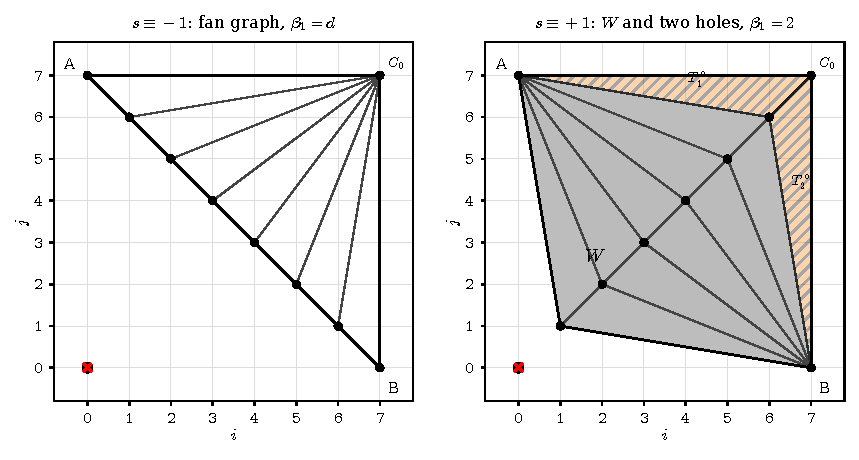
\includegraphics[width=\textwidth]{figures/fig05_special.pdf}
\caption{The two special exceptional configurations for $d=7$. Left: $s\equiv-1$, the fan graph with $d$ bounded triangles ($\beta_1=7$). Right: $s\equiv+1$, the parallelogram $W$, the segments $[A,C_0]$, $[B,C_0]$, $[D_{d-1},C_0]$, and the two open triangles $T_1,T_2$ ($\beta_1=2$).}\label{fig:special}
\par\smallskip\noindent\figdesc{Two panels, each a square $[0,7]^2$. Left: the antidiagonal from $A=(0,7)$ to $B=(7,0)$ with eight points and seven spokes from the upper-right corner $C_0$, no shaded regions. Right: a shaded parallelogram $W$ with vertices $A$, $(1,1)$, $B$, $(6,6)$, plus segments from $C_0$ to $A$, to $B$ and to $(6,6)$, with two white triangles beside $C_0$.}
\end{figure}

\subsection{\texorpdfstring{The overlap at $d=2$}{The overlap at d = 2}}

For $d=2$ the only unit is $1\equiv-1$. Then $F_{Q_0}=\{A=(0,2),\ P_1=(1,1),\ B=(2,0),\ C_0=(2,2)\}$, and the fan description of Proposition~\ref{prop:special-fan} applies: the edges are $[A,P_1]$, $[P_1,B]$ and the spokes $[A,C_0]$, $[P_1,C_0]$, $[B,C_0]$, a graph with four vertices and five edges, so $\beta_1=d=2$. The complement is $\interior T_1\sqcup\interior T_2$ with $T_1=\conv(A,P_1,C_0)$ and $T_2=\conv(B,P_1,C_0)$ of area $1$ each. Thus at $d=2$ the two special descriptions coincide in outcome: $\beta_1=2=d$, and the $s\equiv+1$ construction (which needs $d\ge3$ because $W$ degenerates to a segment) is not used.

\begin{table}[ht]
\centering\small
\begin{tabular}{@{}lll@{}}
\toprule
Class & $U_0$ & $\beta_1(U_0)$\\
\midrule
$d\ge5$, $2\le s\le d-2$ & $H_0$ minus two open triangles & $2$\\
$s\equiv+1$, $d\ge3$ & $W\cup$ three segments; $H_0$ minus two open triangles & $2$\\
$s\equiv-1$, $d\ge3$ & fan graph, no $2$-cells & $d$\\
$d=2$ ($s=1$) & fan graph with $4$ vertices & $2$\\
\bottomrule
\end{tabular}
\caption{Exceptional topology $U_{d,s,(d,d)}$ by modular class (rational coefficients; justified in Section~\ref{sec:topology}).}\label{tab:betti}
\end{table}

%% -------------------------------------------------------------------
\section{Topology, homology and geometric interpretation}\label{sec:topology}

\subsection{Planar topology}

We use Alexander duality in the following form.

\begin{theorem}[Alexander duality; Hatcher, \emph{Algebraic Topology}, Theorem~3.44, \S3.3]\label{thm:alexander}
Let $X$ be a nonempty compact, locally contractible proper subspace of $S^2$. Then $\tilde H_i(S^2\setminus X;\Z)\cong\tilde H^{\,1-i}(X;\Z)$ for all $i$.
\end{theorem}

A compact polyhedron in the plane is locally contractible. We use rational coefficients, where cohomology and homology ranks agree.

\begin{corollary}[Betti numbers of a planar polyhedron]\label{cor:planar-betti}
Let $X\subset\R^2$ be a nonempty compact polyhedron. Then $\beta_1(X)$ equals the number of bounded connected components of $\R^2\setminus X$, and $\beta_2(X)=0$.
\end{corollary}
\begin{proof}
Regard $\R^2\subset S^2=\R^2\cup\{\infty\}$. The set $S^2\setminus X$ is nonempty (it contains $\infty$), and $X$ is a proper compact locally contractible subspace of $S^2$. Theorem~\ref{thm:alexander} with $i=0$ gives $\tilde H_0(S^2\setminus X;\Q)\cong\tilde H^1(X;\Q)$, so $S^2\setminus X$ has exactly $1+\beta_1(X)$ components. One of them contains $\infty$ and the others are the bounded components of $\R^2\setminus X$.

For $\beta_2$, triangulate $X$ and let $z=\sum_\sigma c_\sigma\sigma$ be a $2$-cycle, the $\sigma$ being $2$-simplices of the triangulation oriented as in the plane. Suppose $z\ne0$. Choose a linear functional $\Phi$ on $\R^2$ that is not constant on any edge, and let $v$ be a vertex maximizing $\Phi$ among the vertices of simplices with $c_\sigma\ne0$. At $v$ the simplices of the support of $z$ occupy angular wedges with disjoint interiors, all in the half-plane $\{\Phi\le\Phi(v)\}$ (all their other vertices have smaller $\Phi$). Let $e$ be the edge along the most clockwise bounding ray of the union of these wedges. The simplex $\sigma$ of the support containing $e$ lies counterclockwise from $e$, and no other simplex of the support contains $e$ (it would lie clockwise from $e$). So the coefficient of $e$ in $\partial z$ is $\pm c_\sigma\ne0$, contradicting $\partial z=0$. Hence $H_2(X;\Q)=0$.
\end{proof}

\subsection{Betti numbers of the exceptional union}

\begin{theorem}[Exceptional topology]\label{thm:betti}
$U_0=U_{d,s,(d,d)}$ is connected with $\beta_2(U_0)=0$ and
\[
  \beta_1(U_0)=\begin{cases}
  d & s\equiv-1\pmod d,\\
  2 & \text{otherwise }(d\ge2).
  \end{cases}
\]
(For $d=2$ the two cases coincide, $\beta_1=2=d$.)
\end{theorem}
\begin{proof}
\emph{$s\equiv-1$:} Proposition~\ref{prop:special-fan}.

\emph{Otherwise:} in a nonspecial class and for $s=1$, $d\ge3$, we have $H_0\setminus U_0=\interior T_1\sqcup\interior T_2$ (Theorem~\ref{thm:exceptional}, Proposition~\ref{prop:special-plus}). Then
\[
  \R^2\setminus U_0=(\R^2\setminus H_0)\ \sqcup\ \interior T_1\ \sqcup\ \interior T_2.
\]
Each piece is open and connected: $\R^2\setminus H_0$ is the complement of a compact convex set in the plane, and the triangle interiors are convex. The boundary of each piece is contained in $U_0$: $\partial H_0$ consists of the lower-left chain (in $Z$, resp. in $W$), $[A,C_0]$ and $[B,C_0]$ (edges of $T_1$, $T_2$), all in $U_0$; and $\partial T_i\subseteq U_0$ by \eqref{eq:dT1}. A connected open subset of $\R^2\setminus U_0$ whose boundary lies in $U_0$ is a full component. Therefore $\R^2\setminus U_0$ has exactly three components, of which two are bounded, and Corollary~\ref{cor:planar-betti} gives $\beta_1=2$, $\beta_2=0$. Connectedness: $U_0=Z\cup K\cup\partial T_1\cup\partial T_2$ in a nonspecial class, and these four connected sets meet consecutively ($A\in Z\cap\partial T_1$, $L\in\partial T_1\cap K$, $R\in K\cap\partial T_2$); for $s=1$ it is $W\cup[A,C_0]\cup[B,C_0]\cup[D_{d-1},C_0]$, connected through $A,B,D_{d-1}$. For $d=2$ use Proposition~\ref{prop:special-fan}.
\end{proof}

\subsection{Interpretation: fan versus two holes}

The two exceptional configurations are of different kinds.

\begin{itemize}
\item In the \emph{fan} ($s\equiv-1$) the realized union is one-dimensional. The Graver vectors of $\Gamma_{d,d-1}$ include every $(k,d-k)$, so every fibre point is joined to $C_0$, but the point set has only one point off a line; there is no way to span a nondegenerate parallelogram. The first Betti number counts the $d$ triangular faces of the graph and grows with $d$.
\item In the \emph{two-hole} classes the union is a polygon with two triangular punctures, of fixed first Betti number $2$ independent of $d$ and $s$. The two triangles are the only part of the hull not covered, they have a common vertex $C_0$, and each has area $d/2$, one half of a fundamental parallelogram of $\Gamma$.
\end{itemize}

\begin{remark}[What the topology is a topology of]\label{rem:topology-scope}
The Betti numbers in Theorem~\ref{thm:betti} are Betti numbers of the compact set $U_0$ defined in Section~\ref{sec:cells}. They are not asserted to be forced by occurrence arithmetic: the arithmetic supplies the points and their exact Graver relations, and the cell attachment rule (Remark~\ref{rem:modelling}) is a modelling choice. The abstract complex $K_{\mathrm{abs}}$ of Definition~\ref{def:kabs} has the same underlying set as $U_0$ only after the identification $\pi$; its Betti numbers may differ, for instance if two distinct cells share a boundary and overlap. Statements about the topology of an occurrence fibre are statements about $U_Q$.
\end{remark}

%% -------------------------------------------------------------------
\section{Enlargement and filling of the exceptional holes}\label{sec:fill}

We now show what happens to the two exceptional triangles when the box is enlarged by even one step.

\begin{proposition}[Hole filling]\label{prop:fill}
Let $d\ge3$ and let $s$ be any unit modulo $d$. For every box $Q\ge(d,d)$ with $Q\ne(d,d)$, both closed triangles $T_1,T_2$ lie in $U_Q$.
\end{proposition}
\begin{proof}
By transposition (Proposition~\ref{prop:elem}(5) and Lemma~\ref{lem:T-transpose}) it suffices to treat $Q_2\ge d+1$: if $Q_2=d$ then $Q_1\ge d+1$, and the transposed instance has $Q'_2=Q_1\ge d+1$ and $T_1,T_2$ exchanged.

Let $Q_2\ge d+1$ and put
\[
  R_1=P\bigl(A;\ (c,-1),\ (t,1)\bigr),\qquad R_2=P\bigl((t,1);\ (0,d),\ (c,-1)\bigr).
\]
The generators are Graver by Lemma~\ref{lem:std-graver}, and independent: $\cross((c,-1),(t,1))=c+t=d$ and $\cross((0,d),(c,-1))=-dc\ne0$. The corners of $R_1$ are $A$, $A+(c,-1)=P_{d-t}$, $A+(t,1)=(t,d+1)$ and $A+(d,0)=C_0$; the corners of $R_2$ are $(t,1)$, $(t,d+1)$, $(t,1)+(c,-1)=B$ and $(t,1)+(0,d)+(c,-1)=C_0$. All lie in $\Gamma$, are nonzero, and lie in $[0,d]\times[0,d+1]\subseteq[0,Q_1]\times[0,Q_2]$.

Three corners of $R_1$ are the vertices $A,P_{d-t},C_0$ of $T_1$, so $T_1\subseteq R_1\subseteq U_Q$. Two corners of $R_2$ are $B,C_0$. To see $P_{d-1}=(d-1,a)\in R_2$: write $(d-1,a)=(t,1)+\alpha(0,d)+\beta(c,-1)$. The first coordinate gives $\beta=(d-1-t)/c=(c-1)/c\in[0,1)$ and the second $\alpha=\bigl(a-1+\beta\bigr)/d$. Since $a\ge1$ and $a-1+\beta<a\le d-1$, $\alpha\in[0,1]$. So all vertices of $T_2$ lie in the convex set $R_2$, whence $T_2\subseteq R_2\subseteq U_Q$.
\end{proof}

\begin{figure}[ht]
\centering
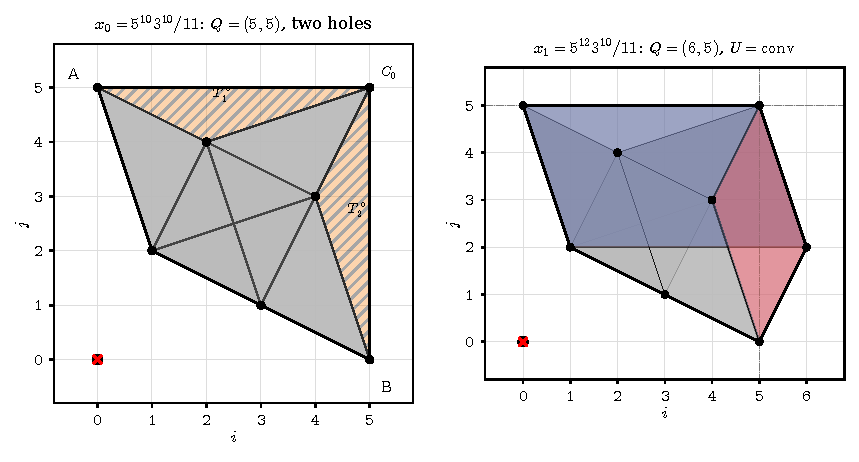
\includegraphics[width=\textwidth]{figures/fig12_example.pdf}
\caption{Hole filling in the running example $(d,s)=(5,2)$ ($t=3$). Left: the exceptional box $Q_0=(5,5)$ with its two white triangles. Right: the box $(6,5)$; the filling cells $R_1,R_2$ are among the cells drawn, together with the cap cells of Part~III. This is the same pair of occurrence fibres as in Section~\ref{sec:example}.}\label{fig:fill-preview}
\par\smallskip\noindent\figdesc{Two side-by-side panels. Left, box $5\times5$: pale parallelograms cover the hull of seven points except two white triangles at the upper right. Right, box $6\times5$: coloured parallelograms cover the entire hull of eight points.}
\end{figure}

\subsection{Old-hull coverage and the dependency chain}

The filling proposition alone does not show that the old hull is covered: one must know what else is missing from $H_0$. In the GEO-I record this was organised as follows.

\begin{itemize}
\item \textbf{G8-T1} is Proposition~\ref{prop:fill}.
\item \textbf{G8-R1} (v008) is the reduction ``$H_0\subseteq U_Q$ for $Q\ge(d,d)$, $Q\ne(d,d)$'' \emph{conditional} on the premise that the complement of $U_0$ in $H_0$ is contained in $T_1\cup T_2$ (called G8-T2 there).
\item The premise is the covering half of the exact complement theorem (v010: G10-Z, G10-T1), which is Theorem~\ref{thm:exceptional} above, together with Proposition~\ref{prop:special-plus} for $s=1$. Combining it with G8-T1 makes G8-R1 unconditional (G10-R1).
\end{itemize}

We give the argument in full.

\begin{corollary}[Old-hull coverage]\label{cor:old}
Let $Q\ge(d,d)$, $Q\ne(d,d)$. If the class is nonspecial, or $s=1$ with $d\ge3$, then $H_0\subseteq U_Q$.
\end{corollary}
\begin{proof}
Every cell admissible for $Q_0$ is admissible for $Q$ (Proposition~\ref{prop:elem}(4)), so $U_0\subseteq U_Q$. By Theorem~\ref{thm:exceptional} (nonspecial) or Proposition~\ref{prop:special-plus} ($s=1$), $H_0\setminus U_0=\interior T_1\sqcup\interior T_2\subseteq T_1\cup T_2$. By Proposition~\ref{prop:fill}, $T_1\cup T_2\subseteq U_Q$. Hence $H_0=U_0\cup(H_0\setminus U_0)\subseteq U_Q$.
\end{proof}

The corollary does not use the formerly conditional statement G8-R1 as an assumption: its single missing premise, the exact description of $H_0\setminus U_0$, is supplied by Theorem~\ref{thm:exceptional} and Proposition~\ref{prop:special-plus}. For $s\equiv-1$ the old hull is also covered, but for a different reason (Theorem~\ref{thm:L}): there $U_0$ is a graph and the old hull is covered only by cells that appear at the first enlargement.

This section finishes the transition inside the original hull. The part of the new hull $H_Q$ outside $H_0$, the \emph{cap}, is covered in Part~III using the arithmetic of Pareto-minimal points.

%% ===================================================================
%% PART III (a): Sections 10-13
%% ===================================================================
\part{Constructive convex stabilization}

This part contains the proof of the universal theorem and of every result on which it depends. The three regimes are: the special classes (Section~\ref{sec:special-stab}), large boxes (Section~\ref{sec:large}), and small boxes in nonspecial classes (Sections~\ref{sec:pareto}--\ref{sec:cap}). They are assembled in Section~\ref{sec:main}.

%% -------------------------------------------------------------------
\section{Stabilization for the special residue classes}\label{sec:special-stab}

\subsection{\texorpdfstring{The Graver bases for $s\equiv\pm1$}{The Graver bases for s = +-1}}

\begin{lemma}[Graver vectors for $s=\pm1$]\label{lem:special-graver}
Let $d\ge2$.
\begin{enumerate}
\item For $s=d-1$ (that is, $\Gamma=\{(i,j):i+j\equiv0\ \mathrm{mod}\ d\}$) the Graver basis is
\[
  \mathcal G=\{\pm(1,-1)\}\ \cup\ \{\pm(k,\,d-k):\ 0\le k\le d\}.
\]
\item For $s=1$ (that is, $\Gamma=\{(i,j):j\equiv i\ \mathrm{mod}\ d\}$) the Graver basis is
\[
  \mathcal G=\{\pm(1,1),\ \pm(d,0),\ \pm(0,d)\}\ \cup\ \{\pm(k,\,-(d-k)):\ 1\le k\le d-1\}.
\]
\end{enumerate}
(For $d=2$ the two descriptions agree.)
\end{lemma}
\begin{proof}
\emph{(1)} Let $g\in\Gamma$ be nonzero. If $g_1g_2<0$ then $g=\pm(m,-n)$ with $m,n>0$ and $(1,-1)\in\Gamma$ satisfies $(1,-1)\conf g$ (up to sign), so $g$ is Graver iff $g=\pm(1,-1)$. Otherwise, after replacing $g$ by $-g$, $g=(m,n)\ge0$ with $m+n=ld$, $l\ge1$ (since $m+n\equiv0$ and $m+n>0$). If $l\ge2$ put $h=(\min(m,d),\ d-\min(m,d))$. Then $h\in\Gamma$ (the sum of its coordinates is $d$), $0\le h\le g$ coordinatewise (if $m<d$ then $d-m\le n$ because $n=ld-m\ge2d-m$), and $h\ne0,g$ since its coordinate sum is $d\ne ld$. So $g$ is not Graver. If $l=1$ every $h\in\Gamma\setminus\{0\}$ with $0\le h\le g$ has coordinate sum a positive multiple of $d$ not exceeding $m+n=d$, hence equal to $d=m+n$, so $h=g$. Thus $g=(m,d-m)$, $0\le m\le d$, is Graver.

\emph{(2)} Let $g\in\Gamma$ be nonzero. If $g_1g_2>0$ then $(1,1)\conf g$ or $(-1,-1)\conf g$, so $g$ is Graver iff $g=\pm(1,1)$. If $g_2=0$ then $g=(m,0)$, $d\mid m$, and $(d,0)\conf g$, so $g$ is Graver iff $g=\pm(d,0)$; likewise for $g_1=0$ and $\pm(0,d)$. If $g_1g_2<0$ write $g=\pm(m,-n)$ with $m,n>0$; $g\in\Gamma$ means $-n\equiv m$, so $m+n=ld$ with $l\ge1$. For $l\ge2$ the vector $h=\pm(\min(m,d),-(d-\min(m,d)))$ is in $\Gamma$, conformally below $g$, and different from $g$ and $0$ (its absolute coordinate sum is $d$); if $\min(m,d)=d$ then $h=\pm(d,0)\conf g$ and the same conclusion holds. For $l=1$ every nonzero $h\conf g$ in $\Gamma$ has absolute coordinate sum a positive multiple of $d$ at most $m+n=d$, hence $h=g$.
\end{proof}

\subsection{The layered coordinate system}

Fix $s\in\{1,d-1\}$, $d\ge2$ and a box $Q$ with $Q_1,Q_2\ge d$. Define the layer function by
\[
  D(i,j)=\frac{i+j}d\quad(s=d-1),\qquad D(i,j)=\frac{j-i}d\quad(s=1).
\]
On $\Gamma$ the function $D$ takes integer values. For an integer $m$ the \emph{layer} $m$ is the set $\Gamma_m=\{z\in\Gamma:D(z)=m\}$. Points of layer $m$ are parametrized by $p=z_1$:
\[
  z=(p,\ md-p)\ \ (s=d-1),\qquad z=(p,\ p+md)\ \ (s=1).
\]
The linear map $z\mapsto(D(z),z_1)$ is invertible, so slices of convex sets by the lines $D=\mathrm{const}$ may be handled in the coordinates $(D,p)$. The points of $F_Q$ in layer $m$ are those with $p\in[\alpha_m,\beta_m]\cap\Z$, where
\[
\begin{array}{c|cc}
 & \alpha_m & \beta_m\\\hline
s=d-1 & \max(0,\,md-Q_2) & \min(Q_1,\,md)\\
s=1 & \max(0,\,-md) & \min(Q_1,\,Q_2-md)
\end{array}
\]
except that for $s=1$ and $m=0$ the origin must be removed, which replaces $\alpha_0=0$ by $\alpha_0=1$. The layers occurring are $1\le m\le M:=\lfloor(Q_1+Q_2)/d\rfloor$ for $s=d-1$ (layer $0$ contains only the origin), and $-\lfloor Q_1/d\rfloor\le m\le\lfloor Q_2/d\rfloor$ for $s=1$.

\begin{lemma}[Slices of the hull]\label{lem:slices}
For every integer layer $m$ in the range above, $H_Q\cap\{D=m\}$ is exactly the segment of points with $p\in[\alpha_m,\beta_m]$. All vertices of $H_Q$ lie at integer values of $D$. Consequently, for each $m$ with layers $m$ and $m+1$ both in range, $H_Q\cap\{m\le D\le m+1\}$ is the convex hull of the two slices at $D=m$ and $D=m+1$, and $H_Q$ is the union of these slabs.
\end{lemma}
\begin{proof}
The segment of lattice points in layer $m$ is contained in $H_Q$, so the slice contains $[\alpha_m,\beta_m]$. Conversely the slice lies in the box, and the intersection of the box with the line $D=m$ is the real interval $[\alpha_m,\beta_m]$ of $p$ (the box constraints on $z_1$ and $z_2$ are exactly the stated lower and upper bounds), except in the case $s=1$, $m=0$, where the box meets the line $D=0$ in the real interval $[0,\min(Q_1,Q_2)]$ containing the origin. For this case let $z\in H_Q\cap\{D=0\}$ be a convex combination of points of $F_Q$, with weights $\tau_0,\tau_+,\tau_-$ on the points of layer $0$, of positive layers, and of negative layers. Write the positive-layer part of $D$ as $\sum w_k m_k$ over points with $m_k\ge1$ and the negative-layer part as $\sum w_k|m_k|$; averaging to $D=0$ makes these equal to a common value $w'$, and $w'\ge\max(\tau_+,\tau_-)\ge(1-\tau_0)/2$. Points of layer $0$ have $z_1\ge1$; points of a negative layer $m\le-1$ have $z_1=p\ge-md\ge d|m|$, because $z_2=p+md\ge0$. Hence
\[
  z_1\ \ge\ \tau_0+d\,w'\ \ge\ \tau_0+\frac d2(1-\tau_0)\ \ge\ 1,
\]
using $d\ge2$. So the origin is not in $H_Q$ and the slice at $D=0$ is $[1,\min(Q_1,Q_2)]$, as claimed. For $s=d-1$ all points of $F_Q$ have $D\ge1$, so $H_Q\subseteq\{D\ge1\}$.

Vertices of $H_Q$ are points of $F_Q$ and have integer $D$. Between consecutive integer values of $D$ the boundary of the convex polygon $H_Q$ has no vertex, so the slab $\{m\le D\le m+1\}\cap H_Q$ is bounded by the two slices and by two straight pieces of the boundary, i.e. it is the convex hull of the two slices.
\end{proof}

\subsection{The theorem}

\begin{theorem}[Stabilization for $s\equiv\pm1$; GEO-I v005, Theorem~L / G5-C1]\label{thm:L}
Let $d\ge2$, $s\in\{1,d-1\}$, $Q_1,Q_2\ge d$ and $Q\ne(d,d)$. Then $U_Q=H_Q$.
\end{theorem}

\begin{proof}
By Lemma~\ref{lem:slices} it suffices to cover each slab between layers $m$ and $m+1$. Write $n_m=\beta_m-\alpha_m+1$ for the number of lattice points in layer $m$.

\emph{Step 1: which layers can have fewer than two points.} Let $s=d-1$. If $md\le\min(Q_1,Q_2)$ then $n_m=md+1\ge3$. If $\max(Q_1,Q_2)\le md$ then $n_m=Q_1+Q_2-md+1$, which is $1$ exactly for $md=Q_1+Q_2$, that is for the top layer $m=M$ when $d\mid Q_1+Q_2$, and $\ge2$ otherwise (as $md<Q_1+Q_2$ for the remaining layers). In between, $n_m=\min(Q_1,Q_2)+1\ge d+1$. So only the top layer can be a singleton, and every other layer in range has at least two points.

Let $s=1$. For $m=0$, $n_0=\min(Q_1,Q_2)\ge d\ge2$. For $m>0$ (and $m\le\lfloor Q_2/d\rfloor$), $n_m=\min(Q_1,Q_2-md)+1$; this is $1$ iff $Q_2=md$, which happens only for the top layer $m=\lfloor Q_2/d\rfloor$, and for lower positive layers $Q_2-md\ge d$ gives $n_m\ge d+1$. For $m<0$ put $m'=-m$: $n_m=\min(Q_1-m'd,Q_2)+1$, equal to $1$ iff $Q_1=m'd$, i.e. only the bottom layer $-\lfloor Q_1/d\rfloor$ when $d\mid Q_1$, and $\ge d+1$ or $\ge2$ otherwise. So only the extreme layers can be singletons. The bottom singleton for $s=1$ is the transpose of the top singleton ($s=1$ has $t=1$, and transposition exchanges $D\leftrightarrow-D$).

\emph{Step 2: slabs between two layers with at least two points each.} Let $m,m+1$ be such layers. Choose integers $p\in[\alpha_m,\beta_m-1]$ and $q\in[\alpha_{m+1},\beta_{m+1}-1]$ and put (in $(D,p)$ coordinates) the four points $X_p=(p,\ \cdot)$, $X_{p+1}$ in layer $m$ and $Y_q,Y_{q+1}$ in layer $m+1$. Explicitly, for $s=d-1$: $X=(p,md-p)$, $Y=(q,(m+1)d-q)$ and $Y-X=(k,d-k)$ with $k=q-p$; for $s=1$: $X=(p,p+md)$, $Y=(q,q+(m+1)d)$ and $Y-X=(k,k+d)$ with $k=q-p$. Consider the parallelogram
\[
  C_{p,q}=P\bigl(X;\ \delta,\ Y-X\bigr),\qquad \delta=(1,-1)\ (s=d-1),\quad\delta=(1,1)\ (s=1).
\]
Its corners are $X,\ X+\delta$ in layer $m$ and $Y,\ Y+\delta$ in layer $m+1$. If $k\in[0,d]$ for $s=d-1$, or $k\in[-d,0]$ for $s=1$, then $Y-X$ is a Graver vector (Lemma~\ref{lem:special-graver}): for $s=d-1$ it is $(k,d-k)$ with $0\le k\le d$; for $s=1$ it is $(k,k+d)$ with $-d\le k\le0$, which is the axis vector $(0,d)$ for $k=0$, the axis vector $(-d,0)$ for $k=-d$, and $-(\kappa,-(d-\kappa))$ with $\kappa=-k\in(0,d)$ otherwise. Also $\delta$ is Graver, and the two are independent ($\cross(\delta,Y-X)=\pm d$). The four corners are in $F_Q$: they lie in layers $m$, $m+1$ with $p,p+1\in[\alpha_m,\beta_m]$ and $q,q+1\in[\alpha_{m+1},\beta_{m+1}]$, and they are nonzero (in layer $m\ne0$ every point is nonzero; in layer $0$ for $s=1$ we have $p\ge\alpha_0=1$). So $C_{p,q}$ is admissible whenever $q-p$ lies in the \emph{band} $[0,d]$ ($s=d-1$) or $[-d,0]$ ($s=1$).

In the coordinates $(D,p)$ the slice of $C_{p,q}$ at $D=m+\theta$, $0\le\theta\le1$, is the interval of length $1$
\[
  \bigl[(1-\theta)p+\theta q,\ (1-\theta)p+\theta q+1\bigr].
\]
The slice of the slab at the same height is $[(1-\theta)\alpha_m+\theta\alpha_{m+1},\ (1-\theta)\beta_m+\theta\beta_{m+1}]$.

Consider lattice paths of pairs $(p,q)$ from $(\alpha_m,\alpha_{m+1})$ to $(\beta_m-1,\beta_{m+1}-1)$ in which each step increases exactly one coordinate by one, all of whose points lie in the band. Such a path exists. The starting and ending pairs are in the band: for $s=d-1$, $\alpha_{m+1}-\alpha_m=\max(0,(m+1)d-Q_2)-\max(0,md-Q_2)\in[0,d]$ and $\beta_{m+1}-\beta_m=\min(Q_1,(m+1)d)-\min(Q_1,md)\in[0,d]$; for $s=1$ the same computation with signs reversed gives differences in $[-d,0]$ (for $m=0$ with $\alpha_0=1$: $\alpha_1-\alpha_0=-1$; for $m=-1$: $\alpha_0-\alpha_{-1}=1-d$). To construct the path, work with $\Delta=q-p$ and the band $[0,d]$ (the case $[-d,0]$ is symmetric). If neither coordinate has reached its final value, increase $p$ if $\Delta\ge1$ and $q$ if $\Delta=0$; the band is respected since $d\ge1$. If $p$ has reached $\beta_m-1$, increase $q$: the new difference is at most $\beta_{m+1}-1-(\beta_m-1)\le d$. If $q$ has reached its final value, increase $p$: the new difference is at least $(\beta_{m+1}-1)-(\beta_m-1)\ge0$.

Along the path, consecutive intervals $[(1-\theta)p+\theta q,\ \cdots+1]$ have starting points differing by $1-\theta$ or by $\theta$, hence by at most $1$, equal to their length, so they overlap or touch. The union is the interval from the first start to the last end, which is exactly the slab slice. Hence the cells $C_{p,q}$ along the path cover the slab.

\emph{Step 3: the singleton top layer, $s=d-1$.} Suppose $Q_1+Q_2=Md$, so the top layer $M$ is the single point $(Q_1,Q_2)$. Layer $M-1$ has $p\in[\max(0,Q_1+Q_2-d-Q_2),\min(Q_1,Q_1+Q_2-d)]=[Q_1-d,Q_1]$ (using $Q_1,Q_2\ge d$), with end points $(Q_1-d,Q_2)$ and $(Q_1,Q_2-d)$. The slab is the triangle with these two points and the apex $(Q_1,Q_2)$. It lies in the parallelogram $P\bigl((Q_1-d,Q_2-d);(d,0),(0,d)\bigr)$, three of whose corners are the vertices of the triangle. This parallelogram is admissible: its generators are the axis Graver vectors, and its base corner $(Q_1-d,Q_2-d)$ lies in $\Gamma$ and in the box and is \emph{nonzero}, since $(Q_1-d,Q_2-d)=0$ would mean $Q=(d,d)$. (This is exactly where the exceptional box is excluded for $s=d-1$.)

\emph{Step 4: the singleton top layer, $s=1$.} Suppose $Q_2=Md$ with $M\ge1$, so layer $M$ is the single point $(0,Md)$. Layer $M-1$ has $p\in[\alpha,d]$ with $\alpha=1$ if $M=1$ (removal of the origin) and $\alpha=0$ if $M\ge2$; its end points are $(\alpha,\alpha+(M-1)d)$ and $(d,Md)$. The slab is the triangle with these two points and the apex $(0,Md)$. It lies in
\[
  P\bigl(w;\ (-d,0),\ (-\alpha,\ d-\alpha)\bigr),\qquad w=(\alpha+d,\ \alpha+(M-1)d),
\]
whose corners are $w$, $w+(-d,0)=(\alpha,\alpha+(M-1)d)$, $w+(-\alpha,d-\alpha)=(d,Md)$ and $w+(-d-\alpha,d-\alpha)=(0,Md)$. The generators are Graver, namely $(-d,0)$ and either $(0,d)$ ($\alpha=0$) or $-(1,-(d-1))$ ($\alpha=1$), and independent. The corner $w$ lies in $\Gamma$; its coordinates are in the box: $\alpha+(M-1)d\le Md=Q_2$ always, and $\alpha+d\le Q_1$ is automatic for $\alpha=0$, while for $\alpha=1$ it means $Q_1\ge d+1$, which holds because $\alpha=1$ forces $M=1$, $Q_2=d$, and $Q\ne(d,d)$. So the parallelogram is admissible and covers the slab. (Again the exceptional box appears here: for $Q=(d,d)$ the corner $w$ would be outside the box.) The case of a singleton bottom layer follows by transposition.

\emph{Step 5: conclusion.} All slabs are covered, so $H_Q\subseteq U_Q$, and $U_Q\subseteq H_Q$ always.
\end{proof}

\begin{remark}[Why the exceptional square is excluded]
For $Q=(d,d)$ the proof of Theorem~\ref{thm:L} fails in exactly one place in each class, and the failure is real. For $s=d-1$ the top layer is $M=2$ with $Q_1+Q_2=2d$, and the cell of Step~3 has the deleted origin $(Q_1-d,Q_2-d)=(0,0)$ as a corner. For $s=1$ the top layer is $M=1$, $\alpha=1$, and the cell of Step~4 needs the corner $w=(d+1,1)$, which is outside the box. Propositions~\ref{prop:special-fan} and \ref{prop:special-plus} show that $U_{(d,d)}\ne H_{(d,d)}$ in both classes. For every other box in the range the same cells are admissible.
\end{remark}

%% -------------------------------------------------------------------
\section{Universal large-box stabilization}\label{sec:large}

\begin{theorem}[Column-strip coverage; GEO-I G7-T1]\label{thm:large}
Let $d\ge2$, $s$ any unit, and $Q_1,Q_2\ge d$ with $\max(Q_1,Q_2)\ge2d$. Then $U_Q=H_Q$.
\end{theorem}

By transposition (Proposition~\ref{prop:elem}(5); the statement is for all units) we may assume $Q_2\ge2d$. For a column index $0\le i\le Q_1$ set
\[
  b_0=d,\qquad b_i=si\bmod d\in\{0,\dots,d-1\}\ (i\ge1),
\]
and
\[
  K_i=\Bigl\lfloor\frac{Q_2-b_i}{d}\Bigr\rfloor,\qquad B_i=(i,b_i),\qquad T_i=B_i+K_i(0,d).
\]

\begin{lemma}[Columns]\label{lem:columns}
\begin{enumerate}
\item The points of $F_Q$ with first coordinate $i$ are exactly $B_i+k(0,d)$, $0\le k\le K_i$, and $K_i\ge1$. So every column contains at least two points, the lowest is $B_i$ and the highest is $T_i$.
\item $b_{i+1}-b_i\in\{s,\ s-d\}$ for all $0\le i<Q_1$. In particular $(1,b_{i+1}-b_i)$ is a Graver vector (Lemma~\ref{lem:std-graver}).
\item (\emph{First claim}) $|K_{i+1}-K_i|\le1$.
\item (\emph{Second claim}) If $K_{i+1}\ne K_i$ then $T_{i+1}-T_i\in\{(1,s),(1,s-d)\}$, hence is a Graver vector.
\end{enumerate}
\end{lemma}
\begin{proof}
(1) The points of $\Gamma$ in column $i$ have ordinates $\equiv si\pmod d$. For $i\ge1$ these are $b_i+kd$, and for $i=0$ they are $kd$ with $k\ge0$, the case $k=0$ being the deleted origin, so the lowest admissible one is $d=b_0$. They lie in the box iff $b_i+kd\le Q_2$, i.e. $k\le K_i$. Since $b_i\le d$ and $Q_2\ge2d$, $K_i\ge\lfloor d/d\rfloor=1$.

(2) For $i\ge1$: $b_{i+1}\equiv b_i+s\pmod d$ and both lie in $[0,d-1]$, so $b_{i+1}-b_i\in(-d,d)$ is congruent to $s$, hence equals $s$ or $s-d$. For $i=0$: $b_1=s$ and $b_0=d$, so the difference is $s-d$.

(3) We have $(Q_2-b_i)/d\in[(Q_2-d)/d,\ Q_2/d]$, an interval of length $1$. The integer parts of two numbers in a closed interval of length $1$ differ by at most $1$.

(4) Write $Q_2=qd+\rho$ with $0\le\rho<d$. Since $b_i\in[0,d]$,
\[
  K_i=q+\Bigl\lfloor\frac{\rho-b_i}d\Bigr\rfloor=\begin{cases}q&b_i\le\rho,\\ q-1&b_i>\rho,\end{cases}
\]
(for $b_i\le\rho$ we have $0\le\rho-b_i<d$, for $b_i>\rho$ we have $-d\le\rho-b_i\le-1$). The ordinate of $T_i$ is $\tau_i=b_i+K_id$. If $K_{i+1}\ne K_i$ then exactly one of $b_i,b_{i+1}$ is $\le\rho$.
\begin{itemize}
\item If $b_i\le\rho<b_{i+1}$, then $b_{i+1}>b_i$, so by (2) $b_{i+1}-b_i=s$, and $\tau_{i+1}-\tau_i=(b_{i+1}+(q-1)d)-(b_i+qd)=s-d$.
\item If $b_{i+1}\le\rho<b_i$, then $b_{i+1}-b_i=s-d$ and $\tau_{i+1}-\tau_i=(b_{i+1}+qd)-(b_i+(q-1)d)=s$.
\end{itemize}
In both cases $T_{i+1}-T_i=(1,\tau_{i+1}-\tau_i)\in\{(1,s-d),(1,s)\}$.
\end{proof}

\begin{figure}[ht]
\centering
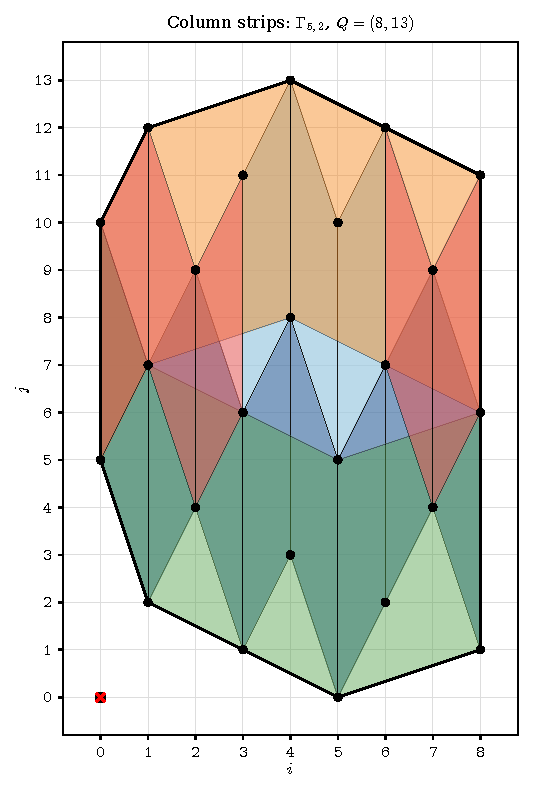
\includegraphics[width=.55\textwidth]{figures/fig06_columns.pdf}
\caption{Column-strip coverage for $d=5$, $s=2$ ($t=3$), $Q=(8,13)$. Blue: stacked translates by $(0,d)$ over each unit slab; red: mismatch triangles where adjacent columns have different heights $K_i\ne K_{i+1}$; green: lower sliver cells (translates of lower-hull pieces by $(0,d)$); purple: upper sliver cells (translates of upper-hull pieces by $(0,-d)$).}\label{fig:columns}
\par\smallskip\noindent\figdesc{A tall rectangle $[0,8]\times[0,13]$ with the hull of the lattice points drawn and tiled almost entirely by blue parallelograms stacked vertically in each unit-wide column, with a few red triangles where neighbouring columns end at different heights, and green and purple strips along the lower and upper boundary.}
\end{figure}

\begin{proof}[Proof of Theorem~\ref{thm:large}]
\emph{Column cells.} Fix a slab $i\le x\le i+1$, $0\le i<Q_1$, and put $\delta=b_{i+1}-b_i$ and $m=\min(K_i,K_{i+1})\ge1$. For $0\le k<m$ the parallelogram
\[
  E_{i,k}=P\bigl(B_i+k(0,d);\ (1,\delta),\ (0,d)\bigr)
\]
has corners $B_i+k(0,d)$, $B_i+(k+1)(0,d)$ in column $i$ and $B_{i+1}+k(0,d)$, $B_{i+1}+(k+1)(0,d)$ in column $i+1$; these are points of $F_Q$ by Lemma~\ref{lem:columns}(1) since $k+1\le m\le K_i,K_{i+1}$. The generators are Graver (Lemma~\ref{lem:columns}(2)) and independent ($\cross=d$). Let $P_B$ be the piecewise linear function with $P_B(i)=b_i$. The cells $E_{i,0},\dots,E_{i,m-1}$ stack and cover $\{P_B\le y\le P_B+md\}$ over the slab.

\emph{Mismatch triangle.} Let $P_T$ be the piecewise linear function with $P_T(i)=\tau_i$ (the ordinate of $T_i$). If $K_i=K_{i+1}$ then $P_T=P_B+md$ on the slab and nothing more is needed. If $K_i\ne K_{i+1}$ then by Lemma~\ref{lem:columns}(3) they differ by exactly $1$, and $P_T-(P_B+md)$ is the linear function equal to $0$ at the end with the smaller $K$ and to $d$ at the other end; the region between is a triangle with vertices $T_i$, $T_{i+1}$ and the point $T_j-(0,d)$ of the taller column $j\in\{i,i+1\}$. Consider
\[
  G_i=P\bigl(T_i;\ T_{i+1}-T_i,\ (0,-d)\bigr),
\]
with corners $T_i,\ T_{i+1},\ T_i-(0,d),\ T_{i+1}-(0,d)$. All four are in $F_Q$ because $K_i,K_{i+1}\ge1$, the generator $T_{i+1}-T_i$ is Graver by Lemma~\ref{lem:columns}(4), and $\cross\bigl(T_{i+1}-T_i,(0,-d)\bigr)=-d$. The triangle is contained in $G_i$, since its three vertices are corners of $G_i$.

\emph{Hull pieces.} Let $l(x)$ and $r(x)$ be the lower and upper ordinates of $H_Q$ at the abscissa $x\in[0,Q_1]$. Since $H_Q$ is a convex polygon with all vertices in $F_Q$, and every column contains at least two points, a vertex of $H_Q$ that is not the lowest point of its column cannot lie on the lower boundary (the lattice point of $F_Q$ just below it is in $H_Q$), and similarly for the upper boundary. Thus every lattice point of $\Gamma$ on the lower boundary of $H_Q$ is a column bottom $B_i$, and every lattice point on the upper boundary is a column top $T_i$. Let $p,p'$ be consecutive boundary lattice points on the lower boundary, with $p_1<p'_1$; they are column bottoms and $p'-p$ is Graver by the boundary Lemma~\ref{lem:reflection}. Put
\[
  S^-(p,p')=P\bigl(p;\ p'-p,\ (0,d)\bigr).
\]
Its corners $p+(0,d)$, $p'+(0,d)$ are in the box because $p_2,p'_2\le d$ and $Q_2\ge2d$, and they are nonzero; so it is admissible ($p'-p$ is not vertical, hence independent of $(0,d)$). It covers $\{l\le y\le l+d\}$ over $[p_1,p'_1]$. Since $0\le l\le P_B\le d$ we have $P_B\le l+d$ and so this cell covers the \emph{lower sliver} $\{l\le y\le P_B\}$. Similarly for consecutive boundary lattice points $p,p'$ on the upper boundary, with $p_1<p'_1$, which are column tops with ordinates $>Q_2-d$, put $S^+(p,p')=P(p;p'-p,(0,-d))$; its corners $p-(0,d)$, $p'-(0,d)$ have ordinates $>Q_2-2d\ge0$ and are in $F_Q$; it covers $\{r-d\le y\le r\}$. Since $P_T\ge Q_2-d\ge r-d$, it covers the \emph{upper sliver} $\{P_T\le y\le r\}$.

\emph{Conclusion.} At every abscissa $x\in[0,Q_1]$ the vertical slice $[l(x),r(x)]$ of $H_Q$ is the union of the lower sliver $[l,P_B]$, the stack $[P_B,P_B+md]$, the mismatch triangle $[P_B+md,P_T]$ and the upper sliver $[P_T,r]$, because $l\le P_B\le P_B+md\le P_T\le r$. Each is covered by an admissible cell. Hence $H_Q\subseteq U_Q$.
\end{proof}

\begin{remark}
The hypothesis $\max(Q_1,Q_2)\ge2d$ is used in four places: the existence of two points in each column, and the three box containments for the shifted cells ($p+(0,d)$ for bottoms, $p-(0,d)$ for tops, and the mismatch cell $G_i$). It is not available in the small-box regime; there the columns may contain a single point, which is why a different mechanism (Sections~\ref{sec:exceptional}--\ref{sec:cap}) is needed.
\end{remark}

%% -------------------------------------------------------------------
\section{An arithmetic inequality for Pareto-minimal points}\label{sec:pareto}

From here on we write $a=d-s$ and $c=d-t$. Note that $ac\equiv st\equiv1\pmod d$.

\begin{definition}[Pareto-minimal point]
A point $M=(x,y)\in\Gamma$ with $0<x,y<d$ is \emph{Pareto-minimal} if $\Gamma\cap([0,x]\times[0,y])=\{0,M\}$.
\end{definition}

A Pareto-minimal point has no other nonzero lattice point weakly below and to the left of it. Every Pareto-minimal point is a Graver vector: a vector $h\in\Gamma$ with $h\conf M$ satisfies $0\le h_1\le x$, $0\le h_2\le y$ (since $M$ has positive coordinates, conformality means the same signs), so $h\in\{0,M\}$.

\begin{lemma}[Arithmetic inequality; GEO-I G12-T1]\label{lem:arith}
Let $s\not\equiv-1\pmod d$ (so that $a,c\ge2$; this includes all nonspecial classes), and let $M=(x,y)$ be Pareto-minimal. Then
\[
  \boxed{\ \max\{\,y+a\,x,\ x+c\,y\,\}\ \ge\ xy.\ }
\]
\end{lemma}
\begin{proof}
Both $y+ax$ and $x+cy$ are positive multiples of $d$: modulo $d$, $y+ax\equiv y-sx\equiv0$ and $x+cy\equiv x-ty\equiv x-tsx\equiv0$. Suppose, to reach a contradiction, that
\[
  y+ax<xy\quad\text{and}\quad x+cy<xy.
\]
\emph{The case $x=1$ (or $y=1$).} If $x=1$ the first inequality reads $y+a<y$, which is false. If $y=1$ the second reads $x+c<x$, which is false. So $x,y\ge2$.

\emph{Consequences of the inequalities.} From $y+ax<xy$ we get $ax<y(x-1)<yx$, so $a<y$. From $x+cy<xy$ we get $c<x$.

\emph{Step 1: $y+ax=d$.} Write $y+ax=bd$ with $b\ge1$. Suppose $b\ge2$. Put $r=\lceil(d-y)/a\rceil$ and $R=(x-r,\ y-d+ar)$. Then:
\begin{itemize}
\item $R\in\Gamma$: $R=M-r(1,s-d)-(0,d)$ and $(1,s-d),(0,d)\in\Gamma$.
\item $r\ge1$ since $y<d$, and $r\le x$ since $y+ax=bd>d$ gives $(d-y)/a<x$; hence $0\le R_1\le x-1$.
\item $R_2\ge0$ because $ar\ge d-y$; and $R_2\le y$ because $ar<(d-y)+a$ gives $R_2<a<y$.
\item $R\ne0$: $R_2+aR_1=y-d+ar+a(x-r)=y+ax-d=(b-1)d>0$.
\end{itemize}
Thus $R$ is a nonzero lattice point of $[0,x]\times[0,y]$ different from $M$ (as $R_1<x$), contradicting Pareto-minimality. Therefore $b=1$.

\emph{Step 2: $x+cy=d$.} Apply Step 1 to the transposed point $(y,x)$ in $\Gamma_{d,t}$, where the roles of $a$ and $c$ are exchanged.

\emph{Step 3: contradiction.} Since $a,c\ge2$, $ac\ge4>1$ and $ac\equiv1\pmod d$, we can write $ac-1=md$ with $m\ge1$. From $y=d-ax$ and $x+cy=d$:
\[
  x+c(d-ax)=d\ \Longrightarrow\ x(ac-1)=d(c-1)\ \Longrightarrow\ mx=c-1.
\]
So $x\le c-1<c$, contradicting $c<x$.
\end{proof}

\begin{remark}[Role of the inequality]
The two numbers $y+ax$ and $x+cy$ are the determinants $\cross(g,M)$ for $g=(1,-a)$ and $g=(c,-1)$ respectively. The lemma says that for at least one of the two Graver vectors $g$ the parallelogram spanned by $g$ and $M$ has area at least $xy$, the area of the rectangle $[0,x]\times[0,y]$. This is exactly the condition under which the bottom cell of Section~\ref{sec:cellfamily} contains the triangle $\Delta_B$.
\end{remark}

\begin{figure}[ht]
\centering
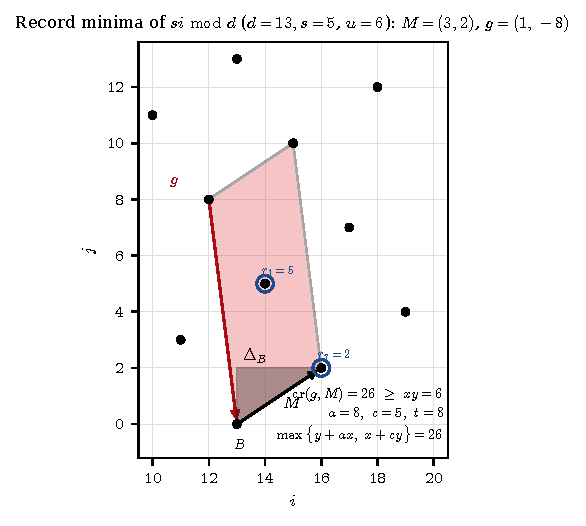
\includegraphics[width=.9\textwidth]{figures/fig07_records.pdf}
\caption{Record minima of $si\bmod d$ and the bottom cell: $d=13$, $s=5$ ($t=8$, $a=8$, $c=5$), $u=6$. The circled points are the records $r_i$; $M=(x,y)$ is the last (smallest) record; $g$ is the chosen Graver vector for which $\cross(g,M)\ge xy$; the shaded parallelogram is $P(B-g;g,M)$ and the dark triangle is $\Delta_B$.}\label{fig:records}
\par\smallskip\noindent\figdesc{A plot of the lattice points of $\Gamma_{13,5}$ to the right of $B=(13,0)$, with the record minima circled in blue and labelled by their ordinates; an arrow $M$ from $B$ to the last record, an arrow $g$ ending at $B$, and a shaded parallelogram with a dark triangle $\Delta_B$ at its right. The lower right corner states the numerical comparison $\cross(g,M)\ge xy$.}
\end{figure}

%% -------------------------------------------------------------------
\section{The boundary Graver reflection theorem}\label{sec:reflection}

\begin{lemma}[Axis pairs are never consecutive]\label{lem:axis-pair}
Let $Q_1,Q_2\ge d$ and let $k,\ell\ge1$ be integers with $kd\le Q_1$ and $\ell d\le Q_2$. Then $(kd,0)$ and $(0,\ell d)$ are not consecutive lattice points on $\partial H_Q$. In particular $B$ and $A$ are never consecutive.
\end{lemma}
\begin{proof}
Suppose they are consecutive. Then the segment between them lies in $\partial H_Q$, and its supporting line $x/(kd)+y/(\ell d)=1$ has $H_Q$ on one side. The point $(kd,\ell d)\in\Gamma$ lies in the box and is nonzero, hence belongs to $F_Q\subseteq H_Q$; the left-hand side equals $2>1$ there. So $x/(kd)+y/(\ell d)\ge1$ on $H_Q$. The points $(d,0)$ and $(0,d)$ are in $F_Q$ since $Q\ge(d,d)$, which gives $1/k\ge1$ and $1/\ell\ge1$, so $k=\ell=1$. Now $(1,s)\in F_Q$ gives $(1+s)/d\ge1$, so $s=d-1$. But then $(1,d-1)$ lies on the open segment between $A$ and $B$, and is a lattice point of $\Gamma$ on $\partial H_Q$ strictly between them, contradicting consecutiveness.
\end{proof}

\begin{lemma}[Boundary Graver lemma; GEO-I G12-T2]\label{lem:reflection}
Let $d\ge2$, $s$ any unit, and $Q_1,Q_2\ge d$ (with no upper bound on $Q$). Let $w,w'$ be two consecutive points of $\Gamma$ on the boundary of $H_Q$, where \emph{all} lattice points of $\Gamma$ on the boundary, including collinear ones, are listed. Then $w'-w$ is a Graver vector.
\end{lemma}

Note that $0\notin H_Q$ (the origin is an extreme point of the quadrant containing $F_Q$, and $F_Q\not\ni0$), so every lattice point on $\partial H_Q$ lies in $F_Q$. Consecutive boundary lattice points lie on a common side of the polygon $H_Q$, since the vertices of $H_Q$ are lattice points.

\begin{proof}
Put $e=w'-w\ne0$ and suppose for contradiction that there is $h\in\Gamma\setminus\{0,e\}$ with $h\conf e$. Put $h'=e-h$; then $h'\in\Gamma\setminus\{0,e\}$ and $h'\conf e$ as well. Let $p=w+h$ and $p'=w'-h=w+h'$. Both lie in the axis-parallel rectangle spanned by $w$ and $w'$, which is contained in the box. They satisfy
\[
  p+p'=w+w'.
\]

\emph{Step 1: $p$ and $p'$ are nonzero.} Suppose $p=0$ (the case $p'=0$ is the same with $w$ and $w'$ exchanged). In each coordinate $i$ with $w_i>0$, $w_i+h_i=0$ gives $h_i=-w_i<0$, so $e_i<0$ by conformality and $|e_i|\ge|h_i|=w_i$, whence $w'_i=w_i+e_i\le0$, i.e. $w'_i=0$. In a coordinate with $w_i=0$ we have $h_i=0$. Since $w\ne0$ some coordinate of $w$ is positive; if both were positive then $w'=0$, impossible. So exactly one coordinate of $w$ is positive; since $w'\ne0$ the other coordinate of $w'$ is positive. As $w,w'\in\Gamma$ and a point of $\Gamma$ on an axis has coordinate divisible by $d$,
\[
  \{w,w'\}=\{(kd,0),\ (0,\ell d)\}\qquad\text{for some integers }k,\ell\ge1.
\]
Both points lie in the box, since $w,w'$ do. This is impossible by Lemma~\ref{lem:axis-pair}, because $w$ and $w'$ are consecutive. So $p,p'\ne0$, hence $p,p'\in F_Q$.

\emph{Step 2: reflection.} Let $\varphi$ be an affine function with $\varphi=0$ on the line through $[w,w']$ and $\varphi\ge0$ on $H_Q$ (a supporting functional). Since $\varphi$ is affine and $p+p'=w+w'$,
\[
  \varphi(p)+\varphi(p')=\varphi(w)+\varphi(w')=0.
\]
Both terms are $\ge0$ because $p,p'\in F_Q\subseteq H_Q$. Hence $\varphi(p)=\varphi(p')=0$: both lie on the supporting line, which meets $H_Q$ in the side containing $[w,w']$.

\emph{Step 3: contradiction.} The vector $h=p-w$ is parallel to $e$, so $h=\theta e$ for some $\theta\in\R$. Conformality $h\conf e$ gives $0\le\theta\le1$, and $h\ne0,e$ gives $0<\theta<1$. Then $p=w+\theta e$ is a lattice point of $\Gamma$ on the open segment between the consecutive boundary lattice points $w$ and $w'$, a contradiction. Therefore no such $h$ exists and $e$ is Graver.
\end{proof}

\begin{remark}[Scope: no upper bound on the box]
The statement and proof hold for \emph{every} box with $Q_1,Q_2\ge d$. The earlier source version of this lemma (GEO-I v012, G12-T2) concluded in Step~1 that $\{w,w'\}=\{B,A\}$ directly, which is only correct when the axis points of $F_Q$ are $A$ and $B$, that is, for $Q<2d$. The argument above does not need this: it handles the axis pairs $(kd,0),(0,\ell d)$ with arbitrary $k,\ell$ by the support argument. This was the correction recorded as D4 in Appendix~\ref{app:corrections}.
\end{remark}

\begin{corollary}[Legitimacy of the cell generators]\label{cor:generators}
Every edge $w\to w'$ of the boundary of $H_Q$ between consecutive lattice points gives a Graver generator $w'-w$ for admissible parallelograms $P(w;w'-w,g)$ and admissible segments, for every Graver $g$ and every translate with corners in $F_Q$. In particular the steps of the lower-left chain (Lemma~\ref{lem:chain0}), the steps of the outer chain $\Omega$ (Section~\ref{sec:chain}) and the hull pieces in the large-box proof are Graver vectors.
\end{corollary}

%% ===================================================================
%% PART III (b): Sections 14-17
%% ===================================================================

\section{The outer hull chain and modular record geometry}\label{sec:chain}

Throughout this section $(d,s)$ is nonspecial and
\[
  Q=(d+u,\ d+v),\qquad 0\le u,v<d,\qquad(u,v)\ne(0,0).
\]
(The persistence result in Section~\ref{sec:persist} holds for all $Q\ge(d,d)$.) Put $H=H_Q$.

\subsection{Persistence of the lower-left hull}\label{sec:persist}

Let $c_0=A,\dots,c_n=B$ be the lower-left chain of $H_0$ and $v_i=(a_i,-b_i)=c_i-c_{i-1}$ its steps (Lemma~\ref{lem:chain0}); these are vectors of $\Gamma$. For each $i$ define
\[
  \varphi_i(z)=\frac{\cross(v_i,z)}{d}=\frac{a_iz_2+b_iz_1}{d},\qquad k_i=\varphi_i(c_{i-1})=\varphi_i(c_i).
\]
By Lemma~\ref{lem:det}, $\varphi_i(z)\in\Z$ for $z\in\Gamma$. The function $\varphi_i$ is increasing in both coordinates, $k_i\ge1$ (as $c_{i-1}\ne0$ lies in the quadrant), and the line $\varphi_i=k_i$ contains the $i$-th edge of the chain; $H_0$ lies in $\{\varphi_i\ge k_i\}$.

\begin{proposition}[Persistence]\label{prop:persist}
For every $Q\ge(d,d)$, every $q\in\Gamma\cap\R_{\ge0}^2\setminus\{0\}$ and every $i$, $\varphi_i(q)\ge k_i$. Consequently $H_Q\subseteq\{\varphi_i\ge k_i\}$ for all $i$, the lower-left chain of $H_0$ lies on $\partial H_Q$, and
\begin{equation}\label{eq:persist}
  H_Q\cap[0,d]^2=H_0.
\end{equation}
\end{proposition}
\begin{proof}
Let $q\in\Gamma$ be nonzero with $q\ge0$. While $q_1>d$ replace $q$ by $q-(d,0)$, and while $q_2>d$ by $q-(0,d)$. Each replacement stays in $\Gamma$ and in the quadrant, keeps $q\ne0$ (the coordinate being reduced stays positive), and strictly decreases every $\varphi_i$, by $a_id/d=a_i>0$ or $b_i>0$ respectively. The process ends at a nonzero point $q^*\in\Gamma\cap[0,d]^2$, that is $q^*\in F_{Q_0}\subseteq H_0$, so $\varphi_i(q)\ge\varphi_i(q^*)\ge k_i$. Thus $F_Q\subseteq\{\varphi_i\ge k_i\}$, and so is the convex hull $H_Q$.

Since the chain points are in $H_Q$ and satisfy $\varphi_i=k_i$ on the $i$-th edge, the edge lies on the supporting line of $H_Q$, hence in $\partial H_Q$. For \eqref{eq:persist}: $H_0\subseteq H_Q\cap[0,d]^2$ is clear. Conversely, the convex polygon $H_0$ is the intersection of the half-planes bounded by its edges, i.e. $H_0=\{x\le d\}\cap\{y\le d\}\cap\bigcap_i\{\varphi_i\ge k_i\}$ (the sides $AC_0$, $C_0B$ and the chain edges), and $H_Q\cap[0,d]^2$ satisfies all these inequalities.
\end{proof}

\begin{remark}
The same argument shows that every nonzero lattice point of the closed quadrant lies on the upper-right side of each supporting line of the chain; the chain is therefore part of the boundary of the convex hull of $\Gamma\cap\R_{\ge0}^2\setminus\{0\}$ (the Klein sail), as claimed in the remark after Theorem~\ref{thm:exceptional}.
\end{remark}

\subsection{\texorpdfstring{The outer chain $\Omega$}{The outer chain Omega}}

By Proposition~\ref{prop:persist}, $\partial H$ is the union of the lower-left chain from $A$ to $B$ and a second arc, from $B$ counterclockwise to $A$, which we call the \emph{outer arc}. Let $\Omega$ be the list of \emph{all} lattice points of $\Gamma$ on the outer arc in order from $B$ to $A$, including collinear ones and the end points $B$ and $A$. Consecutive points of $\Omega$ differ by Graver vectors (Lemma~\ref{lem:reflection}).

Label each $w\in\Omega$:
\[
  \begin{array}{ll}
  R:\ w_1\ge d,\ w_2<d; & C:\ w_1\ge d,\ w_2\ge d;\\
  T:\ w_1<d,\ w_2\ge d; & N:\ w_1<d,\ w_2<d.
  \end{array}
\]
Then $B$ has class $R$ and $A$ has class $T$.

\begin{figure}[ht]
\centering
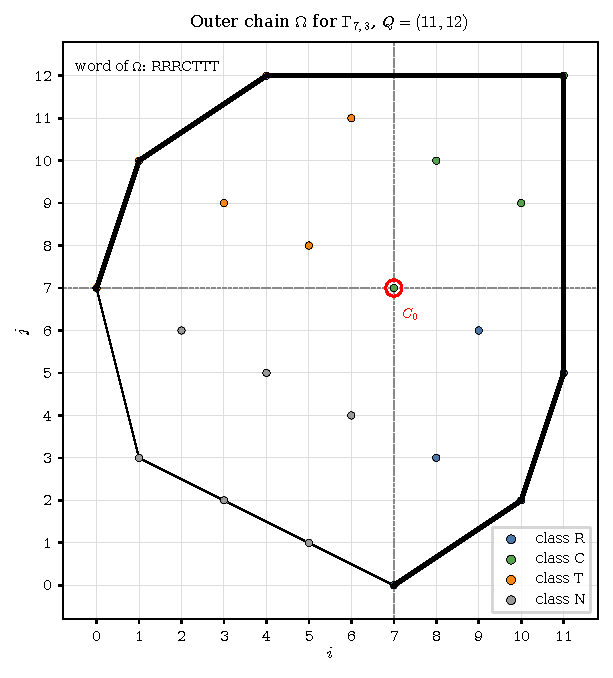
\includegraphics[width=.65\textwidth]{figures/fig08_chain.pdf}
\caption{The outer chain $\Omega$ (thick black) for $d=7$, $s=3$, $Q=(11,12)$, with points coloured by class ($R$ blue, $C$ green, $T$ orange); dashed lines are $x=d$ and $y=d$. Here $\Omega$ has the word $RRRCTTT$ and $C_0=(7,7)$ (red circle) lies in the \emph{interior} of $H_Q$, not on $\Omega$.}\label{fig:chain}
\par\smallskip\noindent\figdesc{A grid with the lattice points of $\Gamma_{7,3}$ in the box $[0,11]\times[0,12]$ coloured by class; the convex hull is outlined and its outer boundary from $B=(7,0)$ counterclockwise to $A=(0,7)$ is drawn thick. Two dashed lines mark $x=7$ and $y=7$ and the point $(7,7)$ is circled in red, inside the hull. The label above the picture spells the word of classes along the chain.}
\end{figure}

\begin{lemma}[Classification of the outer chain]\label{lem:omega}
\begin{enumerate}
\item $\Omega$ contains no point of class $N$.
\item The classes along $\Omega$ form a word in $R^*C^*T^*$.
\item No two consecutive points of $\Omega$ have classes $R$ and $T$ (in this order).
\item Consequently every edge $w\to w'$ of $\Omega$ has both abscissae $\ge d$ or both ordinates $\ge d$ (or both).
\end{enumerate}
\end{lemma}
\begin{proof}
(1) Let $w\in\Omega$ with $w_1,w_2<d$. Then $w\in H\cap[0,d]^2=H_0$ by \eqref{eq:persist}. A point of $H_0$ on $\partial H$ lies on $\partial H_0$ (an interior point of $H_0$ is an interior point of $H\supseteq H_0$). Since $w_1,w_2<d$ it does not lie on the sides $AC_0$ or $C_0B$ of $H_0$, hence lies on the lower-left chain. But the outer arc and the lower-left chain meet only at $A$ and $B$, which have classes $T$ and $R$. Contradiction.

(2) The point $B$ is the lowest point of $H$ (the only point of $\Gamma$ in the box on the $x$-axis other than the origin, because $d\mid x$ and $x<2d$), so counterclockwise from $B$ the outer arc first moves into the half-plane $x\ge d$ (to the right, or up along the side $x=d$ if $u=0$). The vertical line $x=d$ meets $H$ in a chord $[B,B']$, and the boundary of the convex polygon $H\cap\{x\ge d\}$ consists of this chord and one arc of $\partial H$ from $B$ to $B'$. Hence the points of $\Omega$ with $w_1\ge d$ are those on the arc from $B$ to $B'$, an initial segment of $\Omega$. In the same way, the point $A$ is the leftmost point of $H$ (the only point of $\Gamma$ in the box on the $y$-axis other than the origin when $v<d$ is $A$ itself, and $A$ has $x=0$), the line $y=d$ meets $H$ in a chord $[A,A']$, and the points of $\Omega$ with $w_2\ge d$ form the final segment of $\Omega$ from $A'$ to $A$. By (1) every point of $\Omega$ belongs to at least one of these two segments. Points in the initial segment but not the final one are of class $R$, in both of class $C$, in the final one only of class $T$. Since the initial segment is closed under taking predecessors and the final segment under taking successors, all $R$ points precede all $C$ points, which precede all $T$ points. So the word is in $R^*C^*T^*$.

(3) Let $w\in R$ and $w'\in T$ be consecutive. Put $\rho=w+w'-C_0$. Then
\[
  \rho_1=w_1+w'_1-d\in[w'_1,\,w_1),\qquad \rho_2=w_2+w'_2-d\in[w_2,\,w'_2),
\]
because $w'_1<d\le w_1$ and $w_2<d\le w'_2$; so $\rho\in\Gamma$ lies in the rectangle spanned by $w,w'$, inside the box. It is nonzero except possibly if $\rho=0$, which forces $w_1+w'_1=d$ and $w_2+w'_2=d$; with $w_1\ge d$ and $w'_2\ge d$ this gives $w=B$ and $w'=A$, which are never consecutive boundary lattice points of $H_Q$ (Lemma~\ref{lem:axis-pair} with $k=\ell=1$). So $\rho\in F_Q$, and so is $C_0$. Since $\rho+C_0=w+w'$, a supporting functional $\varphi$ of the side through $[w,w']$ satisfies $\varphi(\rho)+\varphi(C_0)=\varphi(w)+\varphi(w')=0$, hence $\varphi(C_0)=0$: the point $C_0$ lies on the supporting line. Its coordinates satisfy $w'_1<d=C_{0,1}\le w_1$ and $w_2<d=C_{0,2}\le w'_2$, so it lies in the rectangle spanned by $w,w'$ and, being on the line through them, on the segment $[w,w']$. It differs from both endpoints (as $w_2<d$ and $w'_1<d$). Thus $C_0$ is a lattice point strictly between consecutive boundary lattice points, a contradiction.

(4) Given (2) and (3), the possible consecutive class pairs are $RR,RC,CC,CT,TT$. In $RR,RC,CC$ both abscissae are $\ge d$; in $CC,CT,TT$ both ordinates are $\ge d$.
\end{proof}

\begin{remark}[The point $C_0$ need not lie on $\Omega$]\label{rem:D9}
Statement~(3) is proved by showing that $C_0$ cannot be a point strictly between two consecutive boundary lattice points of type $R,T$. It does \emph{not} assert that $C_0$ is a vertex of $\Omega$, nor that every $R$-to-$T$ passage runs through $C_0$. In fact $C_0$ can be an interior point of $H_Q$: for $d=5$, $s=2$, $Q=(8,8)$,
\[
  (5,5)=\tfrac19(5,0)+\tfrac13(0,5)+\tfrac59(8,6),
\]
with three points of $F_Q$ not collinear and all weights positive (check: $\frac19\cdot5+\frac59\cdot8=5$ and $\frac13\cdot5+\frac59\cdot6=5$). So $C_0\in\interior H_Q$. The older source text (GEO-I v012, MIXED\_CAP) said that $C_0$ is on a bridging edge of the outer chain; that statement is false and is not used here. This is correction D9 of Appendix~\ref{app:corrections}. In Figure~\ref{fig:chain} the same phenomenon is visible: $C_0$ is interior.
\end{remark}

\subsection{First and last step}

Let $u\ge1$. For $1\le i\le u$ put $r_i=si\bmod d\in\{1,\dots,d-1\}$ (nonzero since $0<i<d$ and $s$ is a unit). The $r_i$ are pairwise distinct (as $i\mapsto si$ is injective mod $d$). Let $y=\min_{1\le i\le u}r_i$, attained at the unique index $x$, and
\[
  M=(x,y).
\]
Since $r_1=s$, $y\le s$; and $x\le u$.

\begin{lemma}[Records]\label{lem:records}
\begin{enumerate}
\item $M\in\Gamma$ is Pareto-minimal; in particular $M$ is a Graver vector.
\item $r_i/i>y/x$ for $1\le i<x$, and $r_i/i\ge y/x$ for $x<i\le u$.
\item The first edge of $\Omega$ is $B\to B+M$; the point $B+M=(d+x,y)$ has class $R$.
\end{enumerate}
\end{lemma}
\begin{proof}
(1) $y\equiv sx$ so $M\in\Gamma$. Let $(i,j)\in\Gamma\cap[0,x]\times[0,y]$. If $i=0$ then $d\mid j\le y<d$, so $j=0$ and the point is the origin. If $1\le i\le x$ ($\le u$) then $j\equiv si$ with $0\le j<d$ gives $j=r_i\ge y$ by minimality of $y$, so $j=y$, $i=x$. Hence $\Gamma\cap[0,x]\times[0,y]=\{0,M\}$. The Graver property was shown after the definition of Pareto-minimality.

(2) For $i<x$: $r_i>y$ (as $x$ is the unique index of the minimum), so $r_i/i>y/x$. For $i>x$ suppose $r_i/i<y/x$ and, among such $i\le u$, take the smallest. Then $r_i\ge y$ and $i'=i-x\ge1$, $r_i-y\equiv si'$, $0\le r_i-y<d$ and $r_i-y\ne0$ (else $d\mid i'$ with $0<i'<d$). So $r_{i'}=r_i-y$ and
\[
  \frac{r_{i'}}{i'}=\frac{r_i-y}{i-x}<\frac yx
\]
(because $r_ix<yi$ implies $x(r_i-y)<y(i-x)$). If $i'>x$ this contradicts the minimality of $i$; if $i'=x$ it contradicts $r_x/x=y/x$; if $i'<x$ it contradicts $r_{i'}/i'>y/x$ from the first part. Hence $r_i/i\ge y/x$ for all $i\le u$.

(3) The points of $F_Q$ with abscissa $d+i$, $1\le i\le u$, have ordinates $\equiv si\pmod d$ and $\ge0$, hence $\ge r_i$; all points of $F_Q$ with abscissa $\le d$ lie above or on the line through $B$ of slope $y/x$ extended to the left (their ordinates are $\ge0$ while the line has negative ordinates there, and $C_0$ lies above it). The displacement from $B$ to $(d+i,j)$ has slope $j/i\ge r_i/i\ge y/x$ by (2). So the line through $B$ and $B+M$ supports $H$, and $B+M=(d+x,y)\in F_Q$ (as $x\le u$ and $y<d\le Q_2$). By Pareto-minimality no lattice point lies strictly between $B$ and $B+M$. Thus $B+M$ is the point following $B$ on the outer arc.
\end{proof}

(Equality in (2) can occur, for example at $i=2x$ if $2y<d$ and $2x\le u$; then $B+2M$ lies on the same supporting line, further from $B$ than $B+M$.)

If $u=0$ there are no points of $F_Q$ with abscissa $>d$; then $Q_1=d$ and the first edge of $\Omega$ runs up the side $x=d$ from $B$ to $C_0$.

\begin{lemma}[Last step]\label{lem:last}
Let $v\ge1$ and let $N=(N_1,N_2)$ be the transposed record: $N_1=\min_{1\le j\le v}(tj\bmod d)$, $N_2$ its unique index $j$. Then $N$ is Pareto-minimal, the point $A+N=(N_1,d+N_2)$ lies in $F_Q$ and has class $T$, and the last edge of $\Omega$ is $A+N\to A$.
\end{lemma}
\begin{proof}
Apply Lemma~\ref{lem:records} to the transposed instance $(d,t,(Q_2,Q_1))$ and transpose back (Proposition~\ref{prop:elem}(5)): the outer arc of the transposed hull is the reversal of the outer arc of $H$, with $B$ and $A$ interchanged.
\end{proof}

%% -------------------------------------------------------------------
\section{Explicit construction of the covering cell family}\label{sec:cellfamily}

Fix a nonspecial class and $Q=(d+u,d+v)$ with $0\le u,v<d$, $(u,v)\ne(0,0)$. Let $\Omega=(w^{(0)}=B,\ w^{(1)},\dots,w^{(\mu)}=A)$.

\begin{table}[ht]
\centering\small
\begin{tabular}{@{}p{3.2cm}p{7.2cm}p{4.2cm}@{}}
\toprule
Family & Cells & Role\\
\midrule
L-cells & $P(w;\,w'-w,\,(-d,0))$ for $\Omega$-edges $w\to w'$ with both abscissae $\ge d$, except the first edge & sweep the cap horizontally\\
D-cells & $P(w;\,w'-w,\,(0,-d))$ for $\Omega$-edges with both ordinates $\ge d$, except the last edge & sweep the cap vertically\\
bottom cell $\mathcal B$ ($u\ge1$) & $P(B-g;\,g,\,M)$ & covers the first-edge region $\Delta_B$\\
left cell $\mathcal A$ ($v\ge1$) & $P(A-h;\,h,\,N)$ & covers the last-edge region $\Delta_A$\\
\bottomrule
\end{tabular}
\caption{The cap family $\mathcal C_Q$ for $Q=(d+u,d+v)$.}\label{tab:capfamily}
\end{table}

\subsection{L-cells and D-cells}

\begin{lemma}[L-cells]\label{lem:L}
Let $w\to w'$ be an edge of $\Omega$ with $w_1,w'_1\ge d$ which is not the first edge ($w\ne B$). Then $P(w;\,w'-w,\,(-d,0))$ is an admissible parallelogram. Its corners are $w,\ w',\ w-(d,0),\ w'-(d,0)$.
\end{lemma}
\begin{proof}
$w'-w$ is Graver by Lemma~\ref{lem:reflection} and $(-d,0)$ is Graver. They are independent: a horizontal vector of $\Gamma$ is divisible by $d$ in its first coordinate, while $w_1,w'_1\in[d,d+u]$ and $u<d$ give $|w'_1-w_1|<d$; so $w'-w$ is horizontal only if it is zero, which it is not. The corners $w-(d,0)$ and $w'-(d,0)$ lie in $\Gamma$ and have abscissae $\ge0$ and ordinates equal to those of $w,w'$, so they lie in the box. They are nonzero: the corner $w-(d,0)$ is zero iff $w=B$, excluded, and $w'-(d,0)=0$ iff $w'=B$, impossible since $B$ is the first point of $\Omega$.
\end{proof}

\begin{lemma}[D-cells]\label{lem:D}
Let $w\to w'$ be an edge of $\Omega$ with $w_2,w'_2\ge d$ which is not the last edge ($w'\ne A$). Then $P(w;\,w'-w,\,(0,-d))$ is admissible.
\end{lemma}
\begin{proof}
The transposed statement of Lemma~\ref{lem:L}, using $v<d$.
\end{proof}

\subsection{The bottom cell and the left cell}

Let $u\ge1$ and $M=(x,y)$ be the record of Lemma~\ref{lem:records}. By Lemma~\ref{lem:arith} one of the two numbers
\[
  \cross\bigl((1,-a),M\bigr)=y+ax,\qquad \cross\bigl((c,-1),M\bigr)=x+cy
\]
is at least $xy$. Choose $g\in\{(1,-a),(c,-1)\}$ with $\cross(g,M)\ge xy$ (if both qualify, take the first). Both vectors are Graver by Lemma~\ref{lem:std-graver}. Define the \emph{bottom cell}
\[
  \mathcal B=P(B-g;\ g,\ M)=B+[0,1]M-[0,1]g.
\]

\begin{lemma}[Bottom cell]\label{lem:bottom}
$\mathcal B$ is admissible and contains the triangle $\Delta_B=\conv\bigl(B,\ B+M,\ (d,y)\bigr)$.
\end{lemma}
\begin{proof}
\emph{Corners.} For $g=(1,-a)$ the corners are $B-g=(d-1,a)$, $B$, $B-g+M=(d-1+x,\,a+y)$ and $B+M=(d+x,y)$. Since $x\le u$ and $y\le s$ we have $d-1+x\le Q_1$ and $a+y\le a+s=d\le Q_2$. For $g=(c,-1)$ they are $(t,1)$, $B$, $(t+x,\,1+y)$ and $B+M$, with $t+x\le d-1+u$ and $1+y\le s+1\le d$. All have positive coordinates, lie in $\Gamma$ (as $g,M\in\Gamma$ and $B\in\Gamma$) and so in $F_Q$. \emph{Independence.} $\cross(g,M)\ge xy>0$.

\emph{Containment.} Relative to $B$ we need $(0,y)=\alpha M-\beta g$ with $\alpha,\beta\in[0,1]$ (the vertices $B$ and $B+M$ of $\Delta_B$ are obviously in $\mathcal B$). Solving the two linear equations,
\[
  \beta=\frac{xy}{\cross(g,M)},\qquad\alpha=\frac{g_1\,y}{\cross(g,M)}.
\]
Here $0<\beta\le1$ by the choice of $g$, and $0<\alpha\le1$ because $\cross(g,M)=g_1y-g_2x=g_1y+|g_2|x\ge g_1y$. Hence $(d,y)\in\mathcal B$ and $\Delta_B\subseteq\mathcal B$ by convexity.
\end{proof}

For $v\ge1$ the \emph{left cell} $\mathcal A$ is defined by transposition: with the record $N=(N_1,N_2)$ of Lemma~\ref{lem:last}, choose $h\in\{(-1,a),(-c,1)\}$ with $\cross(N,h)\ge N_1N_2$ (the two values are $aN_1+N_2$ and $N_1+cN_2$, and one of them is $\ge N_1N_2$ by Lemma~\ref{lem:arith}, applied with $x=N_1$, $y=N_2$), and put
\[
  \mathcal A=P(A-h;\ h,\ N)=A+[0,1]N-[0,1]h.
\]
By transposition, $\mathcal A$ is admissible and contains $\Delta_A=\conv(A,\ A+N,\ (N_1,d))$.

\begin{figure}[ht]
\centering
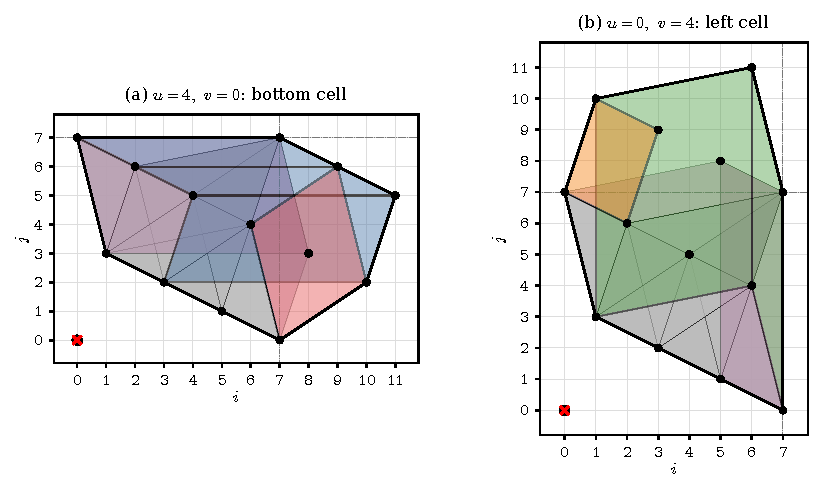
\includegraphics[width=\textwidth]{figures/fig10_endcells.pdf}
\caption{Bottom and left cells, $d=7$, $s=3$. (a) $Q=(11,7)$ ($u=4$, $v=0$): a bottom cell is needed for the first edge. (b) $Q=(7,11)$ ($u=0$, $v=4$): the transposed left cell. All other colours are as in Figure~\ref{fig:sweeps}.}\label{fig:endcells}
\par\smallskip\noindent\figdesc{Two panels. Left: a $11\times7$ box with the convex hull shaded by overlapping cells; a differently coloured parallelogram sits at the lower right corner, adjacent to $B$. Right: the transposed picture, a differently coloured parallelogram at the upper left, adjacent to $A$.}
\end{figure}

\begin{figure}[ht]
\centering
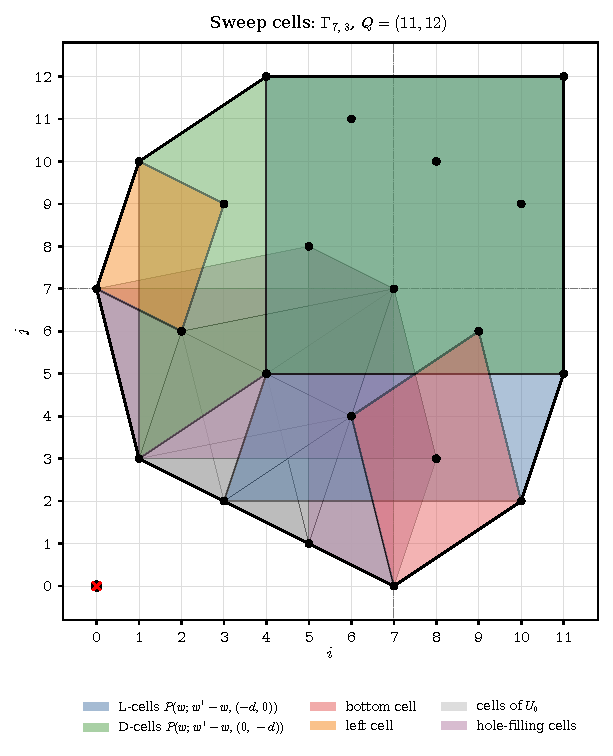
\includegraphics[width=.65\textwidth]{figures/fig09_sweeps.pdf}
\caption{The complete cell family for $d=7$, $s=3$, $Q=(11,12)$ ($u=4$, $v=5$): cells of $U_0$ (grey-green), hole-filling cells $R_1,R_2$ (and transposes), L-cells, D-cells, bottom and left cells. Together with $H_0\subseteq U_Q$ they cover $H_Q$.}\label{fig:sweeps}
\par\smallskip\noindent\figdesc{A $11\times12$ box with the convex hull of the lattice points of $\Gamma_{7,3}$ covered by overlapping coloured parallelograms; the legend below lists the cell families: L-cells, D-cells, bottom cell, left cell, cells of $U_0$, hole-filling cells.}
\end{figure}

%% -------------------------------------------------------------------
\section{Complete coverage of the nonexceptional cap}\label{sec:cap}

\begin{theorem}[Small-box cap coverage; GEO-I G12-T3--T7]\label{thm:cap}
Let $(d,s)$ be nonspecial and $Q=(d+u,d+v)$, $0\le u,v<d$, $(u,v)\ne(0,0)$. Then $H_Q\setminus H_0\subseteq\bigcup\mathcal C_Q$, where $\mathcal C_Q$ is the cap family of Table~\ref{tab:capfamily}. Consequently $U_Q=H_Q$.
\end{theorem}

\subsection{Proof}

\emph{Reduction to generic points.} Let $G$ be the finite set of all horizontal and all vertical lines passing through a lattice point of $\Gamma$ on $\partial H$ (all of them, not only the vertices of $H$), together with the lines $x=d$ and $y=d$. Call a point $z$ \emph{generic} if $z\in\interior H$ and $z\notin\bigcup G$. Generic points are dense in $H$, the union $\bigcup\mathcal C_Q\cup U_0$ is a finite union of closed sets, hence closed, and every point of $H_0$ is in $U_Q$ by Corollary~\ref{cor:old}. So it is enough to show that every generic $z\in H\setminus H_0$ lies in $\bigcup\mathcal C_Q$. By \eqref{eq:persist}, such a $z$ has $z_1>d$ or $z_2>d$. The condition ``generic'' (avoiding the horizontal and vertical lines through \emph{every} boundary lattice point) will be used to place exit points strictly between consecutive boundary lattice points; avoiding only the lines through the vertices of $H$ would not suffice, since the exit point could then be a non-vertex boundary lattice point.

By transposition (which commutes with the cap construction: it exchanges L-cells with D-cells, the bottom cell with the left cell, and the roles of $u,v$, and preserves genericity), the points with $z_1<d<z_2$ follow from the points with $z_2<d<z_1$. So there remain two cases: (1a) $z_1>d>z_2$ and (1b) $z_1>d$, $z_2>d$.

\emph{The horizontal exit point.} Let $z$ be generic with $z_1>d$ (so $u\ge1$). Let $p$ be the point at which the ray $z+\tau(1,0)$, $\tau\ge0$, leaves $H$; $p_1>z_1$ and $p_2=z_2$. Since $z_2$ differs from the ordinate of every boundary lattice point, $p$ is not a boundary lattice point, in particular not a vertex of $H$. Hence $p$ lies in the relative interior of a segment $[w,w']$ joining two \emph{consecutive} boundary lattice points of $H$. This segment is not horizontal, since otherwise $p_2=w_2$.

The point $p$ is the rightmost point of the horizontal slice of $H$ at the height $z_2$. We claim that $[w,w']$ is an edge of the outer chain $\Omega$ in its \emph{ascending part}, that is, the part of $\Omega$ from $B$ up to a highest point of $H$, along which the ordinate is nondecreasing. Indeed, the lowest point of $H$ is $B$ (the only lattice point of the box on the $x$-axis is $B$, since $d\mid x$), so counterclockwise from $B$ the ordinate increases up to the top of $H$ and then decreases; the right ends of the horizontal slices at heights between $0$ and the maximal ordinate lie on the ascending part, and the lower-left chain contains the left ends of its slices. Thus $[w,w']=$ an edge $w\to w'$ of $\Omega$ with $w_2\le w'_2$, and since the edge is not horizontal, $w_2<z_2<w'_2$. By Lemma~\ref{lem:omega}(4), since the edge contains the point $p$ with $p_1>d$, it is of type $RR$, $RC$, $CC$ or $CT$ (type $TT$ has all abscissae $<d$). The key distance estimate is
\begin{equation}\label{eq:dist}
  0<p_1-z_1<Q_1-d=u<d,
\end{equation}
since $p\in H\subseteq[0,Q_1]^2$-box and $z_1>d$.

\emph{Case 1a: $z_1>d>z_2$.} Then $p_2=z_2<d$, so the edge contains a point with ordinate $<d$; edges of type $CC$ and $CT$ have both endpoints with ordinate $\ge d$, hence all their points do. So the edge has type $RR$ or $RC$: both abscissae are $\ge d$.
\begin{itemize}
\item If $w\ne B$, the L-cell $P(w;w'-w,(-d,0))$ of Lemma~\ref{lem:L} is in $\mathcal C_Q$. Its horizontal slice at the height $z_2$ is $[p_1-d,\,p_1]$. By \eqref{eq:dist}, $p_1-d<z_1<p_1$, so $z$ lies in the slice, hence in the cell.
\item If $w=B$, the edge is the first edge $B\to B+M$ (Lemma~\ref{lem:records}), and $z_2\in(0,y)$. The slice of $\Delta_B$ at the height $z_2$ is $[d,\ d+xz_2/y]=[d,p_1]$, which contains $z$ since $d<z_1<p_1$. So $z\in\Delta_B\subseteq\mathcal B$ by Lemma~\ref{lem:bottom}.
\end{itemize}

\emph{Case 1b: $z_1>d$, $z_2>d$.} (Then $v\ge1$.) The edge contains the point $p$ with $p_2=z_2>d$. An $RR$ edge has both ordinates $<d$, so the type is $RC$, $CC$ or $CT$. The first edge $B\to B+M$ has both endpoints of ordinate $<d$ (type $RR$), so $w\ne B$.
\begin{itemize}
\item If the type is $RC$ or $CC$, both abscissae are $\ge d$, the L-cell of the edge is in $\mathcal C_Q$ (Lemma~\ref{lem:L}), and, exactly as in Case~1a using \eqref{eq:dist}, it contains $z$.
\item If the type is $CT$, so $w_1\ge d>w'_1$, both ordinates are $\ge d$. The edge is not the last edge of $\Omega$, which is $A+N\to A$ with starting point of class $T$ (Lemma~\ref{lem:last}), whereas $w$ has class $C$. So the D-cell $P(w;w'-w,(0,-d))$ of Lemma~\ref{lem:D} is in $\mathcal C_Q$. Along this edge, in the direction from $w$ to $w'$, the abscissa decreases (from $\ge d$ to $<d$) and the ordinate is nondecreasing, so the edge is the graph of a decreasing function over $[w'_1,w_1]$, and $H$ lies below and to the left of it (the edge is part of the ascending boundary, with outward normal in the open first quadrant). Since $w'_1<d<z_1<p_1\le w_1$, the vertical line through $z$ meets this edge at the point $q=(z_1,q_2)$ with $q_2\ge p_2=z_2$, and $q_2>z_2$ as $z_1<p_1$. The point $q$ is the top of the vertical slice of $H$ at the abscissa $z_1$, so $q_2\le Q_2=d+v$. Hence
\[
  0<q_2-z_2\le Q_2-z_2<Q_2-d=v<d.
\]
The vertical slice of the D-cell at the abscissa $z_1$ is $[q_2-d,\,q_2]$, which therefore contains $z_2$. So $z$ is in the D-cell.
\end{itemize}
If $v=0$ no generic point has $z_2>d$ and Case 1b is vacuous.

This covers all generic points of $H\setminus H_0$, and by closedness all of $H\setminus H_0$. Together with $H_0\subseteq U_Q$ (Corollary~\ref{cor:old}) we obtain $H_Q\subseteq U_Q$, and $U_Q\subseteq H_Q$ always. \qed

\subsection{Remarks on the proof}

\begin{remark}[Mixed enlargements]
The proof treats $(u,v)$ with $u,v\ge1$, $u\ge1=v-1$, and the one-sided cases $u=0$ or $v=0$ in the same framework. If $v=0$ the last edge of $\Omega$ is $C_0\to A$ (of type $CT$) and nothing above $y=d$ has to be covered; if $u=0$ there are no generic points with $z_1>d$, the first edge of $\Omega$ is $B\to C_0$, and Case~1a is vacuous, while the transposed cases cover the cap above $H_0$.
\end{remark}

\begin{remark}[No residual corner region]
An earlier version of the argument (the GEO-I v011 proof) covered all of the cap except a small polygonal region near $C_0$, a pentagon, which was then treated separately; that pentagon was found to be wrongly described and was corrected. In the present proof no such region arises: every generic point of $H\setminus H_0$ is placed in one of the cells by following a horizontal ray to the ascending right boundary and, if the edge reached crosses $x=d$, a vertical ray to the same edge. In particular the proof never needs to know where $C_0$ lies relative to $\Omega$ (Remark~\ref{rem:D9}).
\end{remark}

\begin{figure}[ht]
\centering
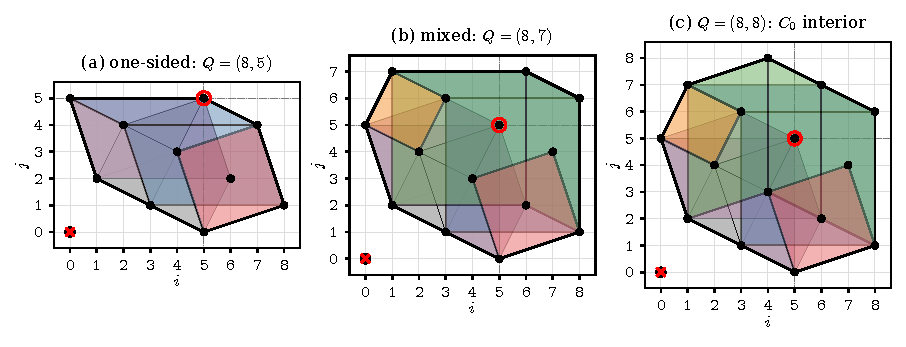
\includegraphics[width=\textwidth]{figures/fig11_cap.pdf}
\caption{Complete coverage for $d=5$, $s=2$: (a) one-sided enlargement $Q=(8,5)$, (b) mixed enlargement $Q=(8,7)$, (c) $Q=(8,8)$, where $C_0=(5,5)$ (red circle) is an interior point of $H_Q$ (correction D9). In each case the coloured cells cover the whole hull.}\label{fig:cap}
\par\smallskip\noindent\figdesc{Three panels with the hull of the lattice points of $\Gamma_{5,2}$ in boxes $8\times5$, $8\times7$, $8\times8$, each completely covered by overlapping coloured parallelograms; in the third panel a red circle marks $(5,5)$ inside the hull.}
\end{figure}

%% -------------------------------------------------------------------
\section{Main theorem: universal planar convex stabilization}\label{sec:main}

\begin{theorem}[Universal planar convex stabilization; GEO-I G12-T8]\label{thm:universal}
For every integer $d\ge2$, every unit $s$ modulo $d$ and every integer box $Q=(Q_1,Q_2)$ with $Q_1,Q_2\ge d$ and $Q\ne(d,d)$,
\[
  \boxed{\,U_{d,s,Q}=\conv\bigl(F_{d,s,Q}\bigr)\,}.
\]
\end{theorem}

\begin{proof}
The proof is a case distinction. The inclusion $U_Q\subseteq H_Q$ always holds (Proposition~\ref{prop:elem}), so only $H_Q\subseteq U_Q$ is to be shown.
\begin{center}
\small
\begin{tabular}{@{}p{5.4cm}p{4.2cm}p{4.8cm}@{}}
\toprule
Parameter regime & Argument & Dependencies\\
\midrule
$s\equiv\pm1$ (all $d\ge2$; this includes every unit for $d=2,3,4,6$) & Theorem~\ref{thm:L} & Lemma~\ref{lem:special-graver}\\
$\max(Q_1,Q_2)\ge2d$ & Theorem~\ref{thm:large} & Lemmas~\ref{lem:columns}, \ref{lem:reflection}\\
$d\ge5$ nonspecial, $Q=(d+u,d+v)$, $0\le u,v<d$ & Corollary~\ref{cor:old} + Theorem~\ref{thm:cap} & Sections~\ref{sec:exceptional}--\ref{sec:fill}, \ref{sec:pareto}--\ref{sec:cellfamily}\\
$Q=(d,d)$ & excluded; classified in Part~II & Theorem~\ref{thm:exceptional}, Propositions~\ref{prop:special-fan}, \ref{prop:special-plus}\\
\bottomrule
\end{tabular}
\end{center}
If $s\equiv\pm1$ apply Theorem~\ref{thm:L}. Otherwise $(d,s)$ is nonspecial, so $d\ge5$. If $\max(Q_1,Q_2)\ge2d$ apply Theorem~\ref{thm:large}. If $\max(Q_1,Q_2)<2d$ then $Q=(d+u,d+v)$ with $0\le u,v<d$ and $(u,v)\neq(0,0)$ since $Q\ne(d,d)$; then $H_0\subseteq U_Q$ by Corollary~\ref{cor:old} and $H_Q\setminus H_0\subseteq U_Q$ by Theorem~\ref{thm:cap}. These cases exhaust the hypotheses.
\end{proof}

\begin{corollary}[Convexity and contractibility]\label{cor:contractible}
Under the hypotheses of Theorem~\ref{thm:universal}, $U_{d,s,Q}$ is a compact convex polygon with vertices in $F_{d,s,Q}$. In particular it is contractible: $\beta_0=1$ and $\beta_k=0$ for $k\ge1$.
\end{corollary}

\begin{corollary}[Persistence of stabilization]\label{cor:persistence}
If $Q\ge(d,d)$, $Q\ne(d,d)$, then $U_{Q'}=H_{Q'}$ for all $Q'\ge Q$. In particular a nonexceptional box never reverts to a nonconvex union as it grows. Together with Theorem~\ref{thm:betti}, the first Betti number of $U_{d,s,Q}$ over all boxes $Q\ge(d,d)$ is $d$ (resp. $2$) at $Q=(d,d)$ for $s\equiv-1$ (resp. otherwise) and $0$ for every other box.
\end{corollary}

\begin{corollary}[Application to an actual planar occurrence fibre]\label{cor:actual}
In the arithmetic setting of Section~\ref{sec:planar}, let $x=a/b$ have two active prime coordinates and assume $d\ge2$,
\[
  q_i\ge o_i\quad(i=1,2),\qquad \bigl(\lfloor q_1/\lambda_1\rfloor,\lfloor q_2/\lambda_2\rfloor\bigr)\ne(d,d).
\]
Then the realized Graver-cell union of the occurrence fibre $F_x\subset\Lambda_b$ equals its convex hull and is contractible. The excluded case is the arithmetic plateau
\[
  o_1\le q_1\le o_1+\lambda_1-1,\qquad o_2\le q_2\le o_2+\lambda_2-1;
\]
there $\beta_1(U)=d$ if $s\equiv-1\pmod d$ and $\beta_1(U)=2$ otherwise.
\end{corollary}
\begin{proof}
By Corollary~\ref{cor:plateau} the hypotheses say $Q_i\ge d$ and $Q\ne(d,d)$ for the normalized box. By Proposition~\ref{prop:transfer} the realized union of the actual fibre is $L(U_{d,s,Q})$, so Theorem~\ref{thm:universal} and Corollary~\ref{cor:contractible} apply. On the plateau Theorem~\ref{thm:betti} applies.
\end{proof}

\begin{remark}[What the theorem does not say]
The theorem does not assert that the admissible cells form a face-to-face subdivision of $H_Q$, or that the abstract complex $K_{\mathrm{abs}}(Q)$ is contractible; it asserts that the \emph{set} $U_Q$ equals the hull. It says nothing for $d=1$, for boxes with a side below $d$, for fibres with three or more active primes, or about the relation between the geometry of different values.
\end{remark}

%% ===================================================================
%% PART IV
%% ===================================================================
\part{Actual occurrence fibres, consequences and literature}

%% -------------------------------------------------------------------
\section{A worked example: two values, two regimes}\label{sec:example}

This section follows two explicit rational numbers through the whole theory. They are
\[
  x_0=\frac{5^{10}\,3^{10}}{11},\qquad x_1=\frac{5^{12}\,3^{10}}{11}.
\]
They are different numbers ($x_1=25\,x_0$) with the same denominator, the same active primes and the same relation lattice. The first sits in the exceptional box and has two holes; the second sits in the nearest larger box and is convex. All numerical data below are exact integers or fractions; they are reproduced by the script \texttt{scripts/example.py} (Appendix~\ref{app:comp}), and are checks of an example, not proofs of the theorems that explain it.

\subsection{\texorpdfstring{The occurrences of $x_0$}{The occurrences of x0}}

By Proposition~\ref{prop:bij}, the occurrences of $x_0$ correspond to the integers $\kappa\ge2$ with $\kappa^2\mid5^{10}3^{10}$ and $\kappa\equiv1\pmod{11}$. Such a $\kappa$ has the form $5^i3^j$ with $0\le i,j\le5$ and $(i,j)\ne(0,0)$. The multiplicative orders modulo $11$ are $\ord_{11}(5)=\ord_{11}(3)=5$ (note $5^5=3125=284\cdot11+1$ and $3^5=243=22\cdot11+1$). We have $3^3=27\equiv5\pmod{11}$, so
\[
  5^i3^j\equiv3^{3i+j}\pmod{11},
\]
which is $1$ if and only if $3i+j\equiv0\pmod5$, that is $j\equiv-3i\equiv2i\pmod5$. This is the planar normalization of Proposition~\ref{prop:norm} with
\[
  D_0=\langle3\rangle=\langle5\rangle,\quad d=5,\quad\lambda_1=\lambda_2=1,\quad g_1=5=3^3=g_2^{-s}\ \Longrightarrow\ s\equiv2\pmod5,
\]
and $t=s^{-1}\equiv3$, $a=d-s=3$, $c=d-t=2$ (the constants of Section~\ref{sec:cells}). The box is $Q=(5,5)=(d,d)$, the exceptional box, because $q_1=q_2=5=o_1=o_2$ lies on the arithmetic plateau of Corollary~\ref{cor:plateau}. Since $d=5$ and $s=2\notin\{1,4\}$, the pair $(d,s)$ is nonspecial.

The fibre is
\[
  F_{x_0}=F_{5,2,(5,5)}=\{(0,5),(1,2),(2,4),(3,1),(4,3),(5,0),(5,5)\},
\]
seven points, shown in Figure~\ref{fig:fibre}. The corresponding occurrences are listed in Table~\ref{tab:example}. For instance $(i,j)=(1,2)$ gives $\kappa=5\cdot9=45=4\cdot11+1$, $N=44$ and
\[
  M=\frac{a}{\kappa^2}\cdot\frac{\kappa-1}{b}=\frac{5^{10}3^{10}}{45^2}\cdot\frac{44}{11}=5^8\,3^6\cdot4=1\,139\,062\,500,
\]
and one checks directly that $M(N+1)^2/N=1\,139\,062\,500\cdot2025/44=5^{10}3^{10}/11$.

\begin{table}[ht]
\centering\small
\begin{tabular}{@{}cr rr rr@{}}
\toprule
$(i,j)$ & $\kappa=5^i3^j$ & $N=\kappa-1$ & $M$ for $x_0$ & $M$ for $x_1$\\
\midrule
$(0,5)$ & $243$ & $242$ & $214\,843\,750$ & $5\,371\,093\,750$\\
$(1,2)$ & $45$ & $44$ & $1\,139\,062\,500$ & $28\,476\,562\,500$\\
$(2,4)$ & $2025$ & $2024$ & $25\,875\,000$ & $646\,875\,000$\\
$(3,1)$ & $375$ & $374$ & $139\,421\,250$ & $3\,485\,531\,250$\\
$(4,3)$ & $16\,875$ & $16\,874$ & $3\,106\,350$ & $77\,658\,750$\\
$(5,0)$ & $3125$ & $3124$ & $16\,769\,916$ & $419\,247\,900$\\
$(5,5)$ & $759\,375$ & $759\,374$ & $69\,034$ & $1\,725\,850$\\
$(6,2)$ & $140\,625$ & $140\,624$ & --- & $9\,319\,536$\\
\bottomrule
\end{tabular}
\caption{The occurrences $(N,M)$ of $x_0=5^{10}3^{10}/11$ (seven rows, column ``$M$ for $x_0$'') and of $x_1=5^{12}3^{10}/11$ (all eight rows). The row $(6,2)$ appears only for $x_1$, since $\kappa^2=5^{12}3^4$ divides $5^{12}3^{10}$ but does not divide $5^{10}3^{10}$.}\label{tab:example}
\end{table}

\subsection{\texorpdfstring{Graver vectors and the realized union of $x_0$}{Graver vectors and the realized union of x0}}

The six standard vectors of Lemma~\ref{lem:std-graver} are Graver vectors of $\Gamma_{5,2}$, and an exhaustive search shows that there are no others (this is special to small moduli: for example $\Gamma_{7,3}$ has the further Graver vector $(3,2)$, Appendix~\ref{app:graver}). Up to sign they are:
\[
  (5,0),\ (0,5),\ (1,2),\ (1,-3),\ (3,1),\ (2,-1).
\]
Each has an arithmetic meaning. The relation $(1,2)$ says $5\cdot3^2=45\equiv1\pmod{11}$; the relation $(1,-3)$ says $5\equiv3^3$; the relation $(2,-1)$ says $5^2\equiv3$; and $(3,1)$ says $5^3\cdot3=375\equiv1$. These are the multiplicative relations among $5$ and $3$ modulo $11$ that cannot be split into two relations of the same sign pattern.

The hull $H_0=\conv F_{x_0}$ has vertices $(0,5),(1,2),(3,1),(5,0),(5,5)$ and area $35/2$. The lower-left chain of Lemma~\ref{lem:chain0} is $A=(0,5)$, $(1,2)$, $(3,1)$, $B=(5,0)$ with steps $(1,-3)$, $(2,-1)$, $(2,-1)$. The zonogon of Lemma~\ref{lem:zonogon} is the parallelogram with vertices $A,(1,2),B,(4,3)$ of area $10$. The additional cell of Lemma~\ref{lem:K} is $K=P\bigl((1,2);(1,2),(3,1)\bigr)$ with corners $(1,2),(2,4),(5,5),(4,3)$. The four cells of the realized union are
\begin{align*}
  C_1&=P\bigl((0,5);(1,-3),(2,-1)\bigr)\ \text{with corners }(0,5),(1,2),(3,1),(2,4),\\
  C_2&=P\bigl((1,2);(1,2),(2,-1)\bigr)\ \text{with corners }(1,2),(2,4),(4,3),(3,1),\\
  C_3&=K,\\
  C_4&=P\bigl((2,4);(1,-3),(2,-1)\bigr)\ \text{with corners }(2,4),(3,1),(5,0),(4,3).
\end{align*}
Each has area $5=d$ (Lemma~\ref{lem:det}), so their areas add to $20$, whereas the area of their union is $25/2$. This is the overlap phenomenon of Example~\ref{ex:overlap}: the cells are distinct admissible parallelograms, not a tiling, and the union is what the theory measures.

The complement $H_0\setminus U_0$ is $\interior T_1\sqcup\interior T_2$ with
\[
  T_1=\conv\bigl((0,5),(2,4),(5,5)\bigr),\qquad T_2=\conv\bigl((5,0),(4,3),(5,5)\bigr),
\]
of area $5/2$ each, so the area of the holes is $5=d$ and $35/2-5=25/2$ is the area of $U_0$, in agreement. The centroids $(7/3,14/3)$ and $(14/3,8/3)$ of the two triangles lie in no admissible cell and on no admissible segment (checked in exact arithmetic). By Theorem~\ref{thm:betti}, $\beta_1(U_0)=2$ and $\beta_2(U_0)=0$.

\subsection{\texorpdfstring{The occurrences of $x_1$: one more point, no holes}{The occurrences of x1: one more point, no holes}}

The number $x_1=5^{12}3^{10}/11$ has $q_1=6$, $q_2=5$, so the normalized box is $Q=(6,5)$. It has one more fibre point, $(6,2)$ (note $2\equiv2\cdot6\bmod5$), and so eight occurrences (Table~\ref{tab:example}). The fibre is the former one together with $(6,2)$, the hull is
\[
  H_1=\conv\bigl((0,5),(1,2),(3,1),(5,0),(6,2),(5,5)\bigr),\qquad\text{area }20.
\]
Here $u=1$, $v=0$, so we are in the one-sided horizontal range of Theorem~\ref{thm:cap}. The outer chain is
\[
  \Omega=\bigl[(5,0),(6,2),(5,5),(0,5)\bigr]\quad\text{with classes }R,R,C,T.
\]
The first boundary step is $M=(1,2)$, the unique record of $2i\bmod5$ for $i\le u=1$, and the Graver vector $g=(1,-3)$ satisfies $\cross(g,M)=5\ge xy=2$. The cells that cover $H_1\setminus H_0$, and in addition the old holes, are:
\begin{itemize}
\item the \emph{bottom cell} $P(B-g;g,M)$ with corners $(4,3),(5,0),(6,2),(5,5)$;
\item the \emph{L-cell} on the edge $(6,2)\to(5,5)$, with corners $(6,2),(5,5),(0,5),(1,2)$;
\item the two \emph{hole-filling cells} (the transposes of $R_1,R_2$ of Proposition~\ref{prop:fill} for $\Gamma_{5,3}$) with corners $(5,0),(4,3),(5,5),(6,2)$ and $(1,2),(6,2),(5,5),(0,5)$.
\end{itemize}
The first filling cell contains $T_2$ and the second contains $T_1$; for instance the vertex $(2,4)$ of $T_1$ lies inside the second one. In exact rational arithmetic the cells $C_1,\dots,C_4$ together with these four cover every point of the grid $\tfrac1{60}\Z^2\cap H_1$ (72\,301 points), as Theorem~\ref{thm:universal} predicts: $U_{5,2,(6,5)}=H_1$. In particular the realized union is convex and contractible, and the first Betti number has fallen from $2$ to $0$ by adding the single occurrence $(6,2)$.

\begin{remark}[The two values are not identified by inclusion]\label{rem:x0x1}
The exponent fibres satisfy $F_{x_0}\subset F_{x_1}$: every index $\kappa$ of an occurrence of $x_0$ is also an index of an occurrence of $x_1$. The occurrences themselves are different pairs. An occurrence determines its value, so no occurrence of $x_0$ is an occurrence of $x_1$. In Table~\ref{tab:example} the index $\kappa$ gives $(N,M)$ for $x_0$ and $(N,25M)$ for $x_1$. Hence the passage from the exceptional box to the next larger one is a statement about two fibres that share a lattice and a box-inclusion, and the identification of the two geometries is made at the level of the normalized lattice $\Gamma_{5,2}$ (Proposition~\ref{prop:transfer}), not at the level of occurrence pairs. This is the mechanism behind Question~\ref{q:global}: nothing in this paper says how the occurrences of different values are related to each other in a way that the geometry sees.
\end{remark}

\begin{remark}[The interior corner]\label{rem:ex-d9}
For the box $Q=(8,8)$ of $\Gamma_{5,2}$ (realized, for example, by $5^{16}3^{16}/11$) the point $C_0=(5,5)$ is an interior point of the hull, by the identity $(5,5)=\tfrac19(5,0)+\tfrac13(0,5)+\tfrac59(8,6)$ of Remark~\ref{rem:D9}, which the script verifies in exact arithmetic. The outer chain of this box therefore does not pass through $C_0$.
\end{remark}

%% -------------------------------------------------------------------
\section{Consequences for occurrence fibres}\label{sec:consequences}

This section collects the statements about actual occurrences that follow from the theorems of Parts~II and~III together with the exact arithmetic of Part~I. Each is a consequence in the strict sense; none introduces a new hypothesis.

\subsection{A threshold law for actual two-prime fibres}

Let $x=a/b$ be a reduced fraction whose numerator has exactly two prime factors $p_1,p_2$ coprime to $b$, with exponent bounds $q_i=\lfloor e_i/2\rfloor\ge1$, and assume $d\ge2$. Put $o_i=\ord_b(p_i)$ and $\lambda_i=o_i/d$. There are three regimes.

\begin{enumerate}
\item \emph{Thin} ($q_i<o_i$ for some $i$). The normalized box has a side below $d$, and our theorems say nothing.
\item \emph{Plateau} ($o_i\le q_i\le o_i+\lambda_i-1$ for $i=1,2$). The normalized box is $(d,d)$. The realized union has $\beta_1=d$ if $s\equiv-1\pmod d$, and $\beta_1=2$ otherwise; it is the fan graph, resp.\ the hull with two open triangles removed.
\item \emph{Convex} ($q_i\ge o_i$ for $i=1,2$ and not on the plateau). The realized union is the whole hull.
\end{enumerate}

This is Corollary~\ref{cor:actual}. It has the form of a threshold law: if one starts on the plateau and raises the exponents of the numerator (replacing $x$ by $xp_1^2$ or $xp_2^2$ repeatedly), the first Betti number of the realized union drops from $2$ (or $d$) to $0$ as soon as some normalized box side exceeds $d$, that is, when some $q_i$ reaches $o_i+\lambda_i$, and it stays $0$ afterwards (Corollary~\ref{cor:persistence}).

\begin{remark}[Sizes]
The plateau is not a small set of values. If $o_1=o_2=d$ (so $\lambda_i=1$) the plateau is the single bound pair $q=(d,d)$, that is, the exponent of $p_i$ in $a$ is $2d$ or $2d+1$. In general it is a rectangle of $\lambda_1\lambda_2$ bound pairs. The plateau is the first place at which both $q_i\ge o_i$ holds, and every value with both $q_i\ge o_i$ lies on it or beyond it.
\end{remark}

\subsection{Realizability and the family of normalized instances}

By Proposition~\ref{prop:realize} every pair $(d,s)$ occurs, with every box. Consequently Theorems~\ref{thm:betti} and~\ref{thm:universal} describe, for each modulus $d$ and each unit $s$, an actual set of values. In particular the two-hole phenomenon is not an artefact of the normalization: for every $d\ge3$ and every unit $s\not\equiv-1$ there is a rational number whose realized union of Graver cells has exactly two bounded complementary components, and the fan graph with $\beta_1=d$ occurs for every $d\ge2$ as the exceptional topology of the $s\equiv-1$ class. We repeat that Proposition~\ref{prop:realize} is an addition of this manuscript and that no result depends on it.

\subsection{Arithmetic meaning of the cells}\label{sec:cell-arith}

Let $w,w'\in F_x$ be two points, $\kappa=\kappa(w)$ and $\kappa'=\kappa(w')$ the corresponding indices. Then $\kappa'/\kappa=p_1^{w'_1-w_1}p_2^{w'_2-w_2}$. Because both indices are $\equiv1\pmod b$, the vector $g=w'-w$ lies in $\Lambda_b$, that is, $p_1^{g_1}p_2^{g_2}\equiv1\pmod b$ (with a negative exponent interpreted in $(\Z/b)^\times$). We distinguish two situations.

\begin{itemize}
\item If $g\ge0$ coordinatewise, then $\kappa\mid\kappa'$ and the quotient $\kappa'/\kappa=p_1^{g_1}p_2^{g_2}$ is itself $\equiv1\pmod b$. Such $g$ is Graver if and only if it is a \emph{minimal} nonnegative relation: no proper divisor of the quotient, other than $1$, is $\equiv1\pmod b$ and of the form $p_1^{h_1}p_2^{h_2}$ with $h\le g$.
\item If $g=(g_1,-g_2)$ with $g_1,g_2>0$ then the relation reads $\kappa'\,p_1^{g_1}=\kappa\,p_2^{g_2}$: two indices related by a common multiple. Graver means minimal for the sign pattern.
\end{itemize}

A cell $P(w;g,h)$ with all four corners in $F_x$ is therefore a ``commuting square'' of occurrences: it records two minimal relations $g$ and $h$ that can be applied in either order, starting from the occurrence $w$, without leaving the set of occurrences. The statement $U=\conv F$ says that every point of the convex hull of the occurrence fibre in exponent space lies in such a commuting square or on a minimal-relation segment. The arithmetic content of the stabilization theorem is thus a statement of local abundance of commuting squares once the box exceeds $(d,d)$, and its failure in the exceptional box is localized in two explicit triangles that have no commuting squares through them.

\begin{remark}[Not a statement about all pairs]
We do not claim that every pair of occurrences in the same fibre is connected by a chain of such squares in the sense of an arithmetic relation among $N$ and $M$. The set $U_Q$ lives in exponent space and records which convex combinations of exponent vectors lie in a cell. How these convex combinations are to be interpreted as arithmetic objects (they are not integers) is not addressed here.
\end{remark}

\subsection{What the theorems determine about the hull}

Since $U_Q=H_Q=\conv F_Q$ beyond the exceptional box, the realized union is a convex lattice polygon with vertices in $F_Q$, and so all its invariants are determined by the extreme points of the fibre. In particular:

\begin{enumerate}
\item the area of $U_Q$ is the area of the polygon, a half-integer because the vertices are integer points; measured in units of the covolume $d$ of $\Gamma$ it is $\operatorname{area}(H_Q)/d$;
\item the boundary of $U_Q$ is the polygonal line through the outer chain $\Omega$ and the lower-left chain, every edge of which is a Graver segment (Lemma~\ref{lem:reflection});
\item $\beta_1(U_Q)=0$ for every box $Q\ge(d,d)$, $Q\ne(d,d)$ (Corollary~\ref{cor:contractible}), so the exceptional first Betti numbers $2$ and $d$ are visible at exactly one box.
\end{enumerate}

In the exceptional box the deficiency $\operatorname{area}(H_0)-\operatorname{area}(U_0)$ equals $d$ in the two-hole classes (two triangles of area $d/2$) and $d^2/2$ (the whole hull) in the class $s\equiv-1$. The jump of the first Betti number and the area deficiency are thus both controlled by the same two triangles $T_1$, $T_2$ of Definition~\ref{def:T}.

\subsection{A structural summary}

Table~\ref{tab:summary} summarises the regimes for the normalized family. The first column gives the box, the second the modular class, the third the realized union and the fourth the theorem that proves it.

\begin{table}[ht]
\centering\small
\begin{tabular}{@{}llll@{}}
\toprule
Box & Class & $U_Q$ & Where proved\\
\midrule
$Q=(d,d)$ & $d\ge5$, $2\le s\le d-2$ & $H_0\setminus(\interior T_1\sqcup\interior T_2)$, $\beta_1=2$ & Thm~\ref{thm:exceptional}, \ref{thm:betti}\\
$Q=(d,d)$ & $s\equiv+1$, $d\ge3$ & $W\cup3$ segments, $\beta_1=2$ & Prop.~\ref{prop:special-plus}\\
$Q=(d,d)$ & $s\equiv-1$, $d\ge2$ & fan graph, $\beta_1=d$ & Prop.~\ref{prop:special-fan}\\
$Q\ge(d,d)$, $Q\ne(d,d)$ & all & $\conv F_Q$, contractible & Thm~\ref{thm:universal}\\
some $Q_i<d$ & all & not treated & ---\\
\bottomrule
\end{tabular}
\caption{The regimes of the realized union for the normalized family $\Gamma_{d,s}$.}\label{tab:summary}
\end{table}

%% -------------------------------------------------------------------
\section{Literature and context}\label{sec:lit}

\paragraph{Scope of this review and a disclosure.}
This review maps the neighbouring mathematics so that a reader can see where the present construction sits. It makes no priority or novelty claim, and no systematic search of the literature on lattice geometry was carried out. The bibliographic data of the works of Graver, Hemmecke, Richter-Gebert--Ziegler, Sturmfels, Schrijver, Ziegler, Beck--Robins and Karpenkov were checked against publisher, society, catalogue or open-access index pages; for these works \emph{only abstracts or catalogue pages were read, not the full texts}, and we have not verified any theorem number inside them. The data for Hatcher and for Bj\"orner--Tancer were taken from a reference list on an encyclopedia page about Alexander duality, and the data for Serre are given from the author's knowledge; they were not checked against a catalogue. Where a sentence below says what a notion is, it records what the cited source's title and abstract lead us to understand, and is not a quotation of a result.

\paragraph{Graver bases and conformal minimality.}
The set of conformally minimal elements of a lattice, taken with respect to the coordinatewise sign-compatible order $h\conf g$ of Definition~\ref{def:conformal}, is the Graver basis of the lattice, introduced by Graver in the study of the foundations of integer linear programming~\cite{Graver1975}. For a lattice of the form $\ker_\Z A$ it is finite. Its connection with toric ideals and Gr\"obner bases is treated in Sturmfels's lecture notes~\cite{Sturmfels1996}; Schrijver's monograph~\cite{Schrijver1986} is a general reference for the integer-programming background. Algorithms for computing Graver bases, among them the positive sum property, are given by Hemmecke~\cite{Hemmecke2003}. In our setting the lattice is two-dimensional, and Lemma~\ref{lem:std-graver} exhibits by hand six Graver vectors, $\pm(d,0)$, $\pm(0,d)$, $\pm(1,s)$, $\pm(1,s-d)$, $\pm(t,1)$, $\pm(d-t,-1)$; the full Graver basis may be larger (Appendix~\ref{app:graver}), and the constructions below use only the Graver property of the generators they employ. What is specific to this paper is not the Graver basis but its use to define an \emph{attachment rule} of parallelogram cells with corners in a finite box fibre.

\paragraph{Parallelograms, zonogons and zonotopal tilings.}
A parallelogram spanned by two vectors is the simplest zonotope, and a zonogon is a Minkowski sum of segments. The classical tilings of zonogons by parallelograms and their correspondence with oriented-matroid data are the subject of the Bohne--Dress theorem; see Richter-Gebert and Ziegler~\cite{RichterGebertZiegler1994} and Ziegler's text on polytopes~\cite{Ziegler1995}. Our zonogon $Z$ of Lemma~\ref{lem:zonogon} is tiled by the sweep of Graver steps of the lower-left hull chain, and the proof there is a direct induction on the number of steps, which includes the case of parallel steps; we have not used the Bohne--Dress theorem. The relation between our sweep tiling and the standard rhombic tilings is plausible but not examined here.

\paragraph{Lattice points in polytopes and the geometry of numbers.}
Enumeration of lattice points in polytopes, including Pick-type area formulas and Ehrhart theory, is covered by Beck and Robins~\cite{BeckRobins2015}. The fibre $F_Q$ is the set of nonzero lattice points of a congruence sublattice in a box, and the hull $H_Q$ is a lattice polygon for the lattice $\Gamma_{d,s}$; the arithmetic inequality of Lemma~\ref{lem:arith} bounds the determinants of triangles spanned by Pareto-minimal points of $\Gamma_{d,s}$ and is, in spirit, a statement of the geometry of numbers. We do not claim a precise relation to the classical theorems (Minkowski's convex body theorem, Dirichlet approximation).

\paragraph{Continued fractions and sails.}
The lower-left chain of Lemma~\ref{lem:chain0} and the record minima of $si\bmod d$ in Section~\ref{sec:pareto} are reminiscent of the sails of Klein polygons and of the continued-fraction expansion of $s/d$; see Karpenkov's book~\cite{Karpenkov2013} on the geometry of continued fractions. The chain of Lemma~\ref{lem:chain0}, with steps $(1,-a)$, \dots, $(c,-1)$ between the points $A$ and $B$, is the boundary of the convex hull of the nonzero lattice points of $\Gamma_{d,s}$ in the positive quadrant, i.e.\ the lower-left part of such a sail, restricted to the box. We have not established a precise dictionary, in particular between the Graver steps and the partial quotients of $s/d$, and we state it only as an analogy.

\paragraph{Homology of planar sets.}
For the topological counts of Section~\ref{sec:topology} we use Alexander duality for compact polyhedra in the plane, in the form of Hatcher~\cite[Theorem~3.44, \S3.3]{Hatcher2002} (the theorem number was confirmed by an independent verification review against an online text, not by us from the printed book). Bj\"orner and Tancer~\cite{BjornerTancer2009} give a short proof of \emph{combinatorial} Alexander duality for simplicial complexes; it is related background and is not used here as a substitute for the topological statement quoted from Hatcher. We state duality only for compact polyhedra in the plane and do not need the general case.

\paragraph{Occurrence arithmetic.}
The occurrence equation $x=M(N+1)^2/N$ is specific to the UNNS nest, and we have not found a direct antecedent in the literature. The reduction to $\kappa^2\mid a$, $\kappa\equiv1\pmod b$ (Proposition~\ref{prop:bij}) is elementary. Congruence lattices as kernels of homomorphisms to $(\Z/b)^\times$ are standard; for the cyclic structure of the unit groups and Dirichlet's theorem, used in Proposition~\ref{prop:realize}, see for example~\cite{Serre1973}.

\paragraph{What is studied here.}
The objects studied in this paper are the occurrence-coordinate correspondence for the fibre of a single rational value, the normalized modular lattices $\Gamma_{d,s}$ obtained from it, and the realized Graver-cell union on the punctured box fibre. The theorems concern this construction only. Comparisons with the topics above are offered as orientation: the lower-left chain is analogous to a sail, the cells are zonotopal, the generators are Graver vectors, and the exceptional holes are the first place where the cell construction fails to reach the convex hull. No further relation is asserted.

\paragraph{Scope note on the term ``arithmetic occurrence geometry''.}
The expression is used here as a defined term (Definition~\ref{def:aog}) for the arithmetic-geometric constructions studied in this work. It is not intended as a synonym for the established field of arithmetic geometry, nor does its use imply a claim of priority over every previous occurrence of similar terminology. We did not survey other fields for similar wording; we understand that phrases of the form ``occurrence geometry'' are used with unrelated meanings elsewhere (for instance for spatial patterns of species occurrence in ecology), and the present meaning is only the one fixed by Definition~\ref{def:aog}.

\subsection{Primary sources: the pinned GEO-I archive}\label{sec:lit-archive}

The mathematical development behind this paper is recorded in twelve archived research releases of the same research programme, GEO-I v001--v012, held in the repository of the UNNS project. All citations below are to the fixed commit
\begin{center}\geoicommit\end{center}
so that a reader can inspect the exact source versions used in preparing the manuscript, even if the main branch later changes. Each release is cited in the bibliography~\cite{GEOIv001,GEOIv002,GEOIv003,GEOIv004,GEOIv005,GEOIv006,GEOIv007,GEOIv008,GEOIv009,GEOIv010,GEOIv011,GEOIv012} as an \emph{archived research release}. These are primary sources for our own programme. They are not independently peer-reviewed publications, and they do not replace the external mathematical literature cited above for Graver bases, lattice geometry, zonogons and algebraic topology. Their role in this paper is given in Table~\ref{tab:geoi-roles}; the precise theorem-level citations are in Table~\ref{tab:geoi-theorems} and in the registry of Appendix~\ref{app:registry}.

\begin{table}[ht]
\centering\small
\begin{tabular}{@{}lp{12.2cm}@{}}
\toprule Release & Role in this paper\\\midrule
v001~\cite{GEOIv001} & Arithmetic occurrence fibres and initial geometric constructions\\
v002~\cite{GEOIv002} & Arithmetic occurrence fibres and initial geometric constructions\\
v003~\cite{GEOIv003} & Abstract versus embedded geometry; finite obstruction theory\\
v004~\cite{GEOIv004} & Abstract versus embedded geometry; planar normalization (Prop.~S1)\\
v005~\cite{GEOIv005} & Special-class stabilization G5-C1 and exceptional topology G5-C2\\
v006~\cite{GEOIv006} & Preliminary modular geometry and computational investigations (context)\\
v007~\cite{GEOIv007} & Large-box theorem G7-T1; exceptional-hole lower bound G7-T3\\
v008~\cite{GEOIv008} & First-enlargement hole filling G8-T1; earlier coverage reduction G8-R1\\
v009~\cite{GEOIv009} & Intermediate geometric results and historical proof development (context)\\
v010~\cite{GEOIv010} & Exact exceptional complement G10-T1; old-hull coverage G10-R1; hull chain G10-L1, G10-Z\\
v011~\cite{GEOIv011} & Intermediate planar results (G11-A etc.) and conjectures, resolved or corrected in v012\\
v012~\cite{GEOIv012} & Pareto inequality G12-T1, boundary Graver theorem G12-T2, cap cover G12-T3--T7, universal stabilization G12-T8\\
\bottomrule
\end{tabular}
\caption{The twelve GEO-I releases and their roles. The principal mathematical sources are v005, v007, v008, v010 and v012; v006, v009 and v011 are historical context.}\label{tab:geoi-roles}
\end{table}

\begin{table}[ht]
\centering\small
\begin{tabular}{@{}p{3.3cm}p{5.4cm}p{5.8cm}@{}}
\toprule Identifier & Release and document & Used in this paper for\\\midrule
G5-C1, G5-C2 & v005~\cite{GEOIv005}, \texttt{STABILIZATION.md} & Theorem~\ref{thm:L}; Proposition~\ref{prop:special-fan}; $\beta_1=2$ for $s=+1$\\
G7-T1 & v007~\cite{GEOIv007}, \texttt{COVERAGE.md} & Theorem~\ref{thm:large}\\
G7-T3 & v007~\cite{GEOIv007}, \texttt{HOLLOW\_TOPOLOGY.md} & Proposition~\ref{prop:hole-exclusion}\\
G8-T1, G8-R1 & v008~\cite{GEOIv008}, \texttt{HOLLOW.md}, \texttt{SMALL\_BOX.md} & Proposition~\ref{prop:fill}; the reduction behind Corollary~\ref{cor:old}\\
G10-T1, G10-T1H, G10-R1, G10-Z, G10-L1 & v010~\cite{GEOIv010}, \texttt{MATHEMATICS.md}, \texttt{HOLLOW.md} & Theorem~\ref{thm:exceptional}; Theorem~\ref{thm:betti}; Corollary~\ref{cor:old}; Lemmas~\ref{lem:chain0}, \ref{lem:zonogon}\\
G12-T1 -- G12-T8, G12-L1, L4, L5 & v012~\cite{GEOIv012}, \texttt{MATHEMATICS.md}, \texttt{MIXED\_CAP.md}, \texttt{GRAVER\_STRIP.md} & Lemmas~\ref{lem:arith}, \ref{lem:reflection}; Theorem~\ref{thm:cap}; Theorem~\ref{thm:universal}\\
\bottomrule
\end{tabular}
\caption{Theorem-level source citations (identifier, release, document). The exact-complement statement of Proposition~\ref{prop:special-plus} is a contribution of this manuscript and is not attributed to v005 (Remark~\ref{rem:s1-source}).}\label{tab:geoi-theorems}
\end{table}

%% ===================================================================
%% PART V
%% ===================================================================
\part{Provenance, verification and open problems}

%% -------------------------------------------------------------------
\section{Provenance and verification}\label{sec:provenance}

The results of this paper have a history, and a reader should be able to tell which kind of evidence stands behind each. This section separates the kinds of evidence. Nothing in it is used in a proof; every theorem of the paper is proved in the text above.

\subsection{Tiers of evidence}\label{sec:tiers}

We use five tiers, and we say which tier each statement belongs to.

\begin{enumerate}[label=\textbf{T\arabic*.},leftmargin=*]
\item \emph{Source-reported proof.} A proof recorded in the GEO-I release series (v004, v005, v007, v008, v010, v012; Section~\ref{sec:lit-archive}) by the author's research programme. We read the relevant statements and, where available, the proofs, but a statement in a release file is not an independently verified result.
\item \emph{Internal written audit.} A re-derivation of the arguments written for this manuscript by the authors of the manuscript (in practice, the model-assisted drafting process described in the acknowledgements below), with the corrections D1--D9 of Appendix~\ref{app:corrections}. Such an audit is a second reading by the same hand. It is not an external review.
\item \emph{Independent computational tests.} Programs written afresh for this manuscript, or for the independent check of its predecessor, which test finite instances of the statements. They are listed in Appendix~\ref{app:comp}. They are \emph{numerical tests}: the geometry is done with the library \texttt{shapely} in double-precision floating point, with an area tolerance of $10^{-9}$; they are not exact certificates. Where exact integer or rational arithmetic is used (the worked example, the Pareto inequality, the realizability check, the boundary-step test), this is said.
\item \emph{External review.} By a human referee or expert. None has taken place.
\item \emph{Formal proof.} Machine-checked formalization in a proof assistant. None has been carried out; it is an optional later activity.
\end{enumerate}

Every theorem of Parts~II and~III is proved in this paper in full, and so in particular has a proof in the sense of tiers~T1 and~T2 combined: a source-reported statement whose proof has been rewritten and audited here. None of them has reached tier~T4 or~T5. This is the honest position of a manuscript that has not yet been refereed.

\subsection{What each theorem rests on}

Appendix~\ref{app:registry} lists each result of this paper next to its identifier in the GEO-I series, its source status as recorded there, and the status of the proof written in this manuscript. Three statements deserve separate mention because they are not simply transcriptions of source proofs:

\begin{itemize}
\item \emph{Proposition~\ref{prop:realize} (realizability)} is an addition of this manuscript. It has a short proof using Dirichlet's theorem on primes in arithmetic progressions. It was tested for all pairs $(d,s)$ with $2\le d\le14$ (29\,127 lattice points compared, no mismatch). No theorem of Parts~II and~III depends on it, and the author may remove it without affecting any other result.
\item \emph{Proposition~\ref{prop:special-plus} (the class $s=+1$)}. The identity $\beta_1=2$ is recorded in the GEO-I series. The exact complement $H_0\setminus U_0=\interior T_1\sqcup\interior T_2$ and its proof from the explicit cell list were derived in the working draft preceding this manuscript. We do not attribute this proposition to the source release.
\item \emph{Lemma~\ref{lem:reflection} (boundary Graver lemma).} The source text concluded in its first step that the reflected point being zero forces $\{w,w'\}=\{B,A\}$, which is correct only for boxes with $Q<2d$; the argument here proves the lemma for all $Q\ge(d,d)$ via Lemma~\ref{lem:axis-pair}. See D4 in Appendix~\ref{app:corrections}.
\end{itemize}

\subsection{Finite computations}

Table~\ref{tab:checks} lists the computations that accompany this paper. All were run on the final texts of the scripts included in the package. The counts are exact counts of tested instances.

\begin{table}[ht]
\centering\small
\begin{tabular}{@{}p{5.2cm}p{4.3cm}rr@{}}
\toprule
Test & Range & Instances & Failures\\
\midrule
Cap cover by the explicit family (Theorem~\ref{thm:cap}), plus old and filling cells & $5\le d\le12$, nonspecial, all $Q=(d+u,d+v)$, $0\le u,v<d$, $(u,v)\neq(0,0)$ & $2130$ & $0$\\
Pareto inequality (Lemma~\ref{lem:arith}), exact integers & nonspecial $5\le d\le120$ & $33\,633$ points & $0$\\
Boundary steps are Graver (Lemma~\ref{lem:reflection}), five boxes per $(d,s)$ & $3\le d\le12$, $Q\le3d$ & $2343$ steps & $0$\\
Full theorem $U_Q=H_Q$ from all admissible parallelograms (Theorem~\ref{thm:universal}), two-dimensional defect only & $2\le d\le8$, $d\le Q_i\le2d+1$, $Q\ne(d,d)$ & $1327$ boxes & $0$\\
Realizability (Proposition~\ref{prop:realize}), exact & $2\le d\le14$, all units & $29\,127$ points & $0$\\
Worked example (Section~\ref{sec:example}), exact rationals & $x_0$, $x_1$; grid of mesh $1/60$ & $72\,301$ points & $0$\\
\bottomrule
\end{tabular}
\caption{Finite computations accompanying this paper (full mode of \texttt{verify\_all.py}). They are support, not proofs. The geometric rows use floating-point geometry with tolerance $10^{-9}$.}\label{tab:checks}
\end{table}

The row on Theorem~\ref{thm:universal} tests only the two-dimensional part of the union (a defect of area above the tolerance), since segments contribute nothing to area; it does not test the Betti numbers. In addition, an independent round of tests written earlier for the preceding working draft reported the following (these were run on that draft, not re-run for this manuscript): the Pareto inequality for all $d\le300$ ($302\,316$ points, no violation); $51\,020$ boundary steps with $Q$ up to $3d+1$, all Graver; the exceptional complement confirmed for $d=3,\dots,11$; $3.67$ million cases of the two intermediate claims of Lemma~\ref{lem:columns}; and full coverage on $2619$ boxes with $d\le10$, no uncovered point.

The GEO-I release records further finite certificates (for instance exact cover of all small boxes up to $d=22$, $29\,206$ boxes; a structure check of the cap decomposition up to $d=16$, $7464$ boxes; $19\,731$ adversarial boxes up to $d=399$; $3000$ random boxes; all with no failure). These are source-reported and were not re-run here.

\subsection{Reconciliation of the historical verification counts (D7)}

The GEO-I records quote several pass counts. As we read the structure of the release files, they are consistent:

\begin{itemize}
\item The v012 verification file lists $27$ entries, and the release's smoke mode reports $25/25$. The $27$ entries are the $25$ new checks of the release together with $2$ gate entries; the smoke mode reports the $25$ checks without the gate entries.
\item The v010 record reports $125/125$ for the mode that was executed, whereas the baseline full gate has $132$ checks. The seven further checks were not part of the executed mode. We re-ran neither mode.
\end{itemize}

We record these counts as history. No number in this paper depends on them, and we do not use them to support any proof.

\subsection{Disclosures about this work}

\begin{enumerate}
\item The GEO-I releases v001--v012 are cited at the fixed commit \geoicommit of the repository (Section~\ref{sec:lit-archive}). The existence of all twelve directories at that commit was checked on GitHub by the author and, in a later verification review, by a reviewer. The drafting process for this manuscript could not itself fetch the repository (the request was refused by the site's robots policy) and read the local copies of the release folders instead; we have not compared the local copies byte for byte with the pinned commit. No frozen release and no repository file was modified.
\item The bibliography was assembled from publisher and catalogue pages (see Section~\ref{sec:lit}); only abstracts or catalogue pages were read.
\item The figures are generated by scripts in the package from exact integer coordinates; the figure captions and descriptions were written by hand and checked against the data (\texttt{figures/figure\_data.json}).
\item Hatcher's Alexander duality is cited as Theorem~3.44, \S3.3; this number was supplied by the verification review (checked there against an online text) and not by us from the printed book. Bj\"orner--Tancer is cited only as background on the combinatorial version.
\item The D7 reconciliation, and the $25/27$ and $125/132$ counts in particular, are our interpretation of the archived release records and have not been independently re-run. The independent verification review of manuscript v1.0 reproduced the smoke mode of \texttt{verify\_all.py}, the worked example and the realizability check; its attempt at the full mode did not finish within its time limit, so the full-mode figures of Table~\ref{tab:checks} rest on the bundled logs.
\end{enumerate}

%% -------------------------------------------------------------------
\section{Open problems}\label{sec:open}

The theorems above close the planar problem for a single fibre in the range $Q\ge(d,d)$. The following questions are open, in the sense that the paper neither proves nor refutes them.

\begin{question}[Global organization across fibres; GEO-I G12-O1]\label{q:global}
Is there a structure on the union over all values $x$ of the occurrence geometries of Parts~II--III, for instance a natural map from the geometry of $x$ to that of $x\,p_i^2$ that respects the cells, or a description of how the exceptional holes of different values lie relative to each other? Remark~\ref{rem:x0x1} shows that the obvious inclusions of exponent fibres do not identify occurrences. The question is whether another identification does.
\end{question}

\begin{question}[Thin boxes]\label{q:thin}
What is the realized union $U_Q$ when one side of the normalized box is below $d$, that is $\min(Q_1,Q_2)<d$? In this range the lattice $\Gamma_{d,s}$ is not sampled over a full period in one direction. We make no claim.
\end{question}

\begin{question}[Three or more active primes]\label{q:higher}
For $k\ge3$ prime coordinates, the relation lattice $\Lambda_b$ is a lattice in $\Z^k$, with Graver basis possibly large. Is there an analogue of the exceptional box, with cells replaced by Graver zonotopes, and a stabilization theorem? Our proofs are planar throughout: they use the cyclic order of the boundary, the determinant $\cross$, and the Alexander duality count in the plane.
\end{question}

\begin{question}[Embedded versus realized]\label{q:embedded}
For which $(d,s,Q)$ do the admissible cells of $U_Q$ form a face-to-face subdivision of the hull, so that $K_{\mathrm{abs}}=K_{\mathrm{emb}}=U_Q$? By Example~\ref{ex:overlap} this fails already at $(5,2,(5,5))$. What are the Betti numbers of $K_{\mathrm{abs}}$, and are they determined by $(d,s,Q)$ in the same way as those of $U_Q$?
\end{question}

\begin{question}[Dictionary with continued fractions]\label{q:cf}
Can the Graver steps of the lower-left chain and the records of Section~\ref{sec:pareto} be expressed in terms of the continued-fraction expansion of $s/d$, and does the arithmetic inequality of Lemma~\ref{lem:arith} follow from classical properties of convergents? We state this only as a question.
\end{question}

\begin{question}[Formal verification]\label{q:formal}
Lemmas~\ref{lem:arith} and~\ref{lem:reflection} are finite combinatorial arguments with an explicit case split. They are natural targets for a machine-checked formalization, which would raise them to tier~T5 of Section~\ref{sec:tiers}. The same applies to the covering arguments of Section~\ref{sec:cap}, which are longer.
\end{question}

\paragraph{Acknowledgements.}
The drafting, proof re-derivations, scripts and figures of this manuscript were produced in a collaboration between the author and an AI assistant (Claude, Anthropic). The mathematical programme, the source releases and all decisions on content are the author's. No external funding or external review is acknowledged.


\appendix
%% ===================================================================
%% APPENDICES
%% ===================================================================

%% -------------------------------------------------------------------
\section{Notation and reconciliation with the source releases}\label{app:notation}

\subsection{Notation}

Table~\ref{tab:notation-app} fixes the notation of the paper. Sections~\ref{sec:arith} and~\ref{sec:planar} use $a/b$ for the reduced fraction $x$; from Section~\ref{sec:exceptional} on the letter $a$ denotes $d-s$ and $c$ denotes $d-t$ (the constants of the lower-left chain), and the numerator is no longer used.

\begin{table}[ht]
\centering\small
\begin{tabular}{@{}p{4.6cm}p{10.4cm}@{}}
\toprule
Symbol & Meaning\\
\midrule
$(N,M)$, $\kappa=N+1$ & an occurrence and its index; $x=M(N+1)^2/N$\\
$x=a/b$, $e_i$, $q_i=\lfloor e_i/2\rfloor$ & reduced fraction, exponents of the numerator, exponent bounds\\
$D(x)$, $\Lambda_b=\ker\chi_b$ & set of occurrence indices; relation lattice of the primes modulo $b$\\
$F_x$ & fibre in prime-exponent coordinates: nonzero lattice points of $\Lambda_b$ in the box $[0,q]$\\
$r_i,o_i,D_0,d,\lambda_i,g_i$ & residue of $p_i$, its order, intersection subgroup, planar modulus, scale factors, normalized generators\\
$\Gamma_{d,s}$, $s$, $t=s^{-1}$, $a=d-s$, $c=d-t$ & modular lattice $\{(i,j):j\equiv si\ (\mathrm{mod}\ d)\}$, unit, inverse, chain constants\\
$Q=(Q_1,Q_2)$, $u=Q_1-d$, $v=Q_2-d$ & normalized box and its excess over the exceptional box\\
$F_Q=F_{d,s,Q}$, $H_Q=\conv F_Q$, $U_Q$ & punctured fibre, hull, realized union of Graver cells\\
$Q_0=(d,d)$, $H_0,U_0,F_0$ & the exceptional box and its objects\\
$A=(0,d)$, $B=(d,0)$, $C_0=(d,d)$ & the three exceptional corners (note: $A$ and $B$ are interchanged in the v005 notation)\\
$P_i=(i,\,si\bmod d)$ & the points of $F_0$ other than $A,B,C_0$ (Lemma~\ref{lem:exc-fibre})\\
$T_1,T_2$ & the exceptional triangles of Definition~\ref{def:T}, each of area $d/2$\\
$\cross(g,h)=g_1h_2-g_2h_1$ & determinant; $\cross(g,h)\equiv0\pmod d$ on $\Gamma_{d,s}$\\
$h\conf g$ & conformal order: $h_ig_i\ge0$ and $|h_i|\le|g_i|$\\
$P(w;g,h)$ & parallelogram with corners $w,w+g,w+g+h,w+h$\\
$\Omega$ & the outer chain of boundary lattice points of $H_Q$ from $B$ to $A$\\
$R,C,T,N$ & classes of a lattice point $w$ by $(w_1\ge d?,\ w_2\ge d?)$: $R$ if $w_1\ge d>w_2$, $C$ if both, $T$ if $w_2\ge d>w_1$, $N$ if neither\\
\bottomrule
\end{tabular}
\caption{Notation.}\label{tab:notation-app}
\end{table}

\subsection{Reconciliation with the GEO-I release notation}

The releases use release-local notation. We record the differences that affect reading the sources. No release file was changed.

\begin{itemize}
\item v001 uses $d$ for the occurrence index ($\kappa$ here); the planar modulus $d$ appears only in v004 and later.
\item v005 interchanges the roles of $A$ and $B$: its $A$ is $(d,0)$ in our notation.
\item v007 uses $u=(d-t,-1)$ for a Graver vector; here $u$ is the horizontal excess of the box and the vector is written $(c,-1)$.
\item v012 \S0 states some elementary facts (finiteness, closedness, monotonicity, inclusion in the hull, transposition) without proof, and writes a shorthand ``every box'' for the stabilization range; the correct range is $Q\ge(d,d)$, $Q\ne(d,d)$ (correction D1).
\item The releases call the realized set simply ``$U$'' and do not distinguish $K_{\mathrm{abs}}$, $U_Q$ and $K_{\mathrm{emb}}$; Definition~\ref{def:kabs} introduces the distinction.
\end{itemize}

\subsection{Corrections D1--D9}\label{app:corrections}

During the preparation of the working draft and of this manuscript nine issues were found in the way the source material is stated or argued. In each case the mathematics in this paper is corrected or completed; the source releases are unchanged. We list them with the place where they are treated.

\begin{description}
\item[D1 (scope of special-class stabilization).] Theorem~L of v005 holds for $Q\ge(d,d)$ and $Q\ne(d,d)$. In the exceptional box it is false for the fan graph and for $s=+1$ ($d\ge3$). Treated in Section~\ref{sec:special-stab} (Theorem~\ref{thm:L}) and Section~\ref{sec:special-classes}.
\item[D2 (special cases are not trivial).] The classes $s\equiv\pm1$ must be treated separately, with their own Graver bases and their own exceptional topology; they are not dismissed as degenerate. Sections~\ref{sec:special-classes} and~\ref{sec:special-stab}.
\item[D3 (exact complement for $s=+1$).] The source gives $\beta_1=2$ but not the exact complement; Proposition~\ref{prop:special-plus} derives it from the cell list.
\item[D4 (scope of the reflection lemma).] The source argument for the case in which the reflected point is zero is correct only for $Q<2d$. Lemma~\ref{lem:axis-pair} and Lemma~\ref{lem:reflection} prove the statement for all $Q\ge(d,d)$ by a support argument.
\item[D5 (old-hull coverage).] The source reduction G8-R1 is conditional on a premise (old-hull coverage) that is supplied by the exact classification of the exceptional box (Theorem~\ref{thm:exceptional}). The dependency chain is made explicit in Section~\ref{sec:fill}, and Corollary~\ref{cor:old} is unconditional.
\item[D6 (boundary lemmas).] The source registry omits two of the lemmas used for the structure of the outer chain, and the argument that $B,A$ are never consecutive. They are supplied in Section~\ref{sec:chain} and Lemma~\ref{lem:axis-pair}.
\item[D7 (verification counts).] Historical counts are reconciled in Section~\ref{sec:provenance}; they play no role in any proof.
\item[D8 (symbols).] The clashes listed above are resolved by the notation of this paper.
\item[D9 (location of $C_0$).] The source text asserts that $C_0$ lies on the outer chain or on a bridging edge. This is false: for $d=5$, $s=2$, $Q=(8,8)$, $(5,5)=\frac19(5,0)+\frac13(0,5)+\frac59(8,6)$ is an interior point of the hull (Remark~\ref{rem:D9}). In $\statInterior$ of the $\statTotal$ boxes $Q=(d+u,d+v)$ with $5\le d\le8$, nonspecial $s$ and $(u,v)\ne(0,0)$, the point $C_0$ is strictly interior to $H_Q$ (Appendix~\ref{app:boundary}). The proof of the cap theorem does not use the false statement.
\end{description}

%% -------------------------------------------------------------------
\section{Arithmetic details}\label{app:arith}

\subsection{\texorpdfstring{Small examples of $D(x)$}{Small examples of D(x)}}

\begin{itemize}
\item $x=36$ ($a=36$, $b=1$): $\kappa^2\mid36$ gives $\kappa\in\{2,3,6\}$ and every $\kappa\equiv1\pmod1$, so $D(36)=\{2,3,6\}$ and the occurrences are $(1,9),(2,8),(5,5)$.
\item $x=225/4$: $\kappa^2\mid225$ gives $\kappa\in\{3,5,15\}$; $\kappa\equiv1\pmod4$ leaves only $\kappa=5$. So $D(x)=\{5\}$ and the unique occurrence is $(N,M)=(4,\ \tfrac{225}{25}\cdot\tfrac44)=(4,9)$, and indeed $9\cdot25/4=225/4$.
\item $x=1$: $a=1$ has no $\kappa\ge2$ with $\kappa^2\mid a$, so $D(1)=\varnothing$.
\end{itemize}

\subsection{Normalization data}

Table~\ref{tab:param} gives the normalization data for a range of pairs of primes. The columns $d,\lambda_1,\lambda_2,s$ were computed from the orders and from the generators $g_i=r_i^{\lambda_i}$ exactly as in Proposition~\ref{prop:norm}, and in each row the equivalence $p_1^{\lambda_1i}p_2^{\lambda_2j}\equiv1\iff j\equiv si\pmod d$ was checked for $0\le i,j<2d$.

\begin{longtable}{@{}rrr rr r rr r@{}}
\toprule $b$ & $p_1$ & $p_2$ & $o_1$ & $o_2$ & $d$ & $\lambda_1$ & $\lambda_2$ & $s$\\\midrule\endhead
11 & 2 & 3 & 10 & 5 & 5 & 2 & 1 & 1\\
11 & 3 & 5 & 5 & 5 & 5 & 1 & 1 & 3\\
11 & 2 & 5 & 10 & 5 & 5 & 2 & 1 & 2\\
11 & 5 & 7 & 5 & 10 & 5 & 1 & 2 & 4\\
11 & 3 & 7 & 5 & 10 & 5 & 1 & 2 & 3\\
13 & 2 & 3 & 12 & 3 & 3 & 4 & 1 & 2\\
13 & 2 & 5 & 12 & 4 & 4 & 3 & 1 & 1\\
13 & 5 & 7 & 4 & 12 & 4 & 1 & 3 & 3\\
13 & 3 & 7 & 3 & 12 & 3 & 1 & 4 & 1\\
19 & 2 & 3 & 18 & 18 & 18 & 1 & 1 & 11\\
19 & 3 & 5 & 18 & 9 & 9 & 2 & 1 & 4\\
19 & 2 & 5 & 18 & 9 & 9 & 2 & 1 & 1\\
19 & 5 & 7 & 9 & 3 & 3 & 3 & 1 & 1\\
19 & 3 & 7 & 18 & 3 & 3 & 6 & 1 & 2\\
29 & 2 & 3 & 28 & 28 & 28 & 1 & 1 & 11\\
29 & 3 & 5 & 28 & 14 & 14 & 2 & 1 & 11\\
29 & 2 & 5 & 28 & 14 & 14 & 2 & 1 & 5\\
29 & 5 & 7 & 14 & 7 & 7 & 2 & 1 & 1\\
29 & 3 & 7 & 28 & 7 & 7 & 4 & 1 & 3\\
31 & 2 & 3 & 5 & 30 & 5 & 1 & 6 & 1\\
31 & 3 & 5 & 30 & 3 & 3 & 10 & 1 & 1\\
31 & 5 & 7 & 3 & 15 & 3 & 1 & 5 & 2\\
31 & 3 & 7 & 30 & 15 & 15 & 2 & 1 & 1\\
\bottomrule\caption{Normalization data $(d,s,\lambda_1,\lambda_2)$ of Proposition~\ref{prop:norm} for some primes $p_1,p_2$ and denominators $b$ (computed; the congruence $p_1^{\lambda_1i}p_2^{\lambda_2j}\equiv1\iff j\equiv si\pmod d$ was verified for $0\le i,j<2d$ in each row; rows with $d=1$ omitted).}\label{tab:param}\end{longtable}

\subsection{\texorpdfstring{A normalization with $\lambda_1>1$}{A normalization with lambda1 > 1}}

Take $b=11$, $p_1=2$, $p_2=3$ (the first row of Table~\ref{tab:param}): $\ord_{11}(2)=10$, $\ord_{11}(3)=5$, $D_0=\langle3\rangle$ (the subgroup of order $5$), $d=5$, $\lambda_1=2$, $\lambda_2=1$, $g_1=2^2=4$, $g_2=3$. We have $4=3^{-1}\cdot$? Indeed $3^4=81\equiv4$, so $g_1=g_2^4=g_2^{-1}$, hence $-s\equiv-1$ and $s\equiv1\pmod5$. The relation lattice is $\Lambda_{11}=\{(2i,j):j\equiv i\pmod5\}$; for instance $(2,1)\in\Lambda_{11}$ corresponds to $2^2\cdot3=12\equiv1$. If $x=2^{2q_1}3^{2q_2}/11$ with $q_1=10$, $q_2=5$ then $Q=(\lfloor10/2\rfloor,5)=(5,5)$: the exceptional box for a special class $s=1$. For $q_1=11$ one still has $Q_1=5$ (the plateau of Corollary~\ref{cor:plateau}: $o_1=10\le q_1\le o_1+\lambda_1-1=11$), and for $q_1=12$ one has $Q=(6,5)$.

%% -------------------------------------------------------------------
\section{Graver calculations}\label{app:graver}

Lemma~\ref{lem:std-graver} proves that six explicit vectors are always Graver vectors, and Lemma~\ref{lem:special-graver} gives the complete Graver basis for $s=\pm1$. For other classes the Graver basis can contain further vectors. As a cross-check, Table~\ref{tab:graver} lists, for $3\le d\le9$, the complete Graver basis obtained by exhaustive search for conformally minimal elements of $\Gamma_{d,s}\cap[-d,d]^2$ (Lemma~\ref{lem:graver-size} says that $|g_i|\le d$ for every Graver vector, so this search is complete). The tag ``the six standard vectors only'' means that the basis consists of exactly those; ``extra vectors'' that it does not (this includes $s=\pm1$, where the list is that of Lemma~\ref{lem:special-graver}, and nonspecial classes from $d=7$ on, for example $(7,3)$ with the extra vector $(3,2)$). Nothing in the proofs depends on the basis being the six standard vectors: the exclusion of the exceptional triangles (Proposition~\ref{prop:hole-exclusion}) is proved for arbitrary Graver vectors, and the covering cells use only the Graver property of the vectors they employ.

\begin{longtable}{@{}rrp{9.2cm}@{}}
\toprule $d$ & $s$ & Graver vectors of $\Gamma_{d,s}$ up to sign (computed by exhaustive conformal minimality in $[-d,d]^2$)\\\midrule\endhead
3 & 1 & $(0,3)$, $(1,-2)$, $(1,1)$, $(2,-1)$, $(3,0)$ (the six standard vectors only; 5 vectors)\\
3 & 2 & $(0,3)$, $(1,-1)$, $(1,2)$, $(2,1)$, $(3,0)$ (the six standard vectors only; 5 vectors)\\
4 & 1 & $(0,4)$, $(1,-3)$, $(1,1)$, $(2,-2)$, $(3,-1)$, $(4,0)$ (extra vectors; 6 vectors)\\
4 & 3 & $(0,4)$, $(1,-1)$, $(1,3)$, $(2,2)$, $(3,1)$, $(4,0)$ (extra vectors; 6 vectors)\\
5 & 1 & $(0,5)$, $(1,-4)$, $(1,1)$, $(2,-3)$, $(3,-2)$, $(4,-1)$, $(5,0)$ (extra vectors; 7 vectors)\\
5 & 2 & $(0,5)$, $(1,-3)$, $(1,2)$, $(2,-1)$, $(3,1)$, $(5,0)$ (the six standard vectors only; 6 vectors)\\
5 & 3 & $(0,5)$, $(1,-2)$, $(1,3)$, $(2,1)$, $(3,-1)$, $(5,0)$ (the six standard vectors only; 6 vectors)\\
5 & 4 & $(0,5)$, $(1,-1)$, $(1,4)$, $(2,3)$, $(3,2)$, $(4,1)$, $(5,0)$ (extra vectors; 7 vectors)\\
6 & 1 & $(0,6)$, $(1,-5)$, $(1,1)$, $(2,-4)$, $(3,-3)$, $(4,-2)$, $(5,-1)$, $(6,0)$ (extra vectors; 8 vectors)\\
6 & 5 & $(0,6)$, $(1,-1)$, $(1,5)$, $(2,4)$, $(3,3)$, $(4,2)$, $(5,1)$, $(6,0)$ (extra vectors; 8 vectors)\\
7 & 1 & $(0,7)$, $(1,-6)$, $(1,1)$, $(2,-5)$, $(3,-4)$, $(4,-3)$, $(5,-2)$, $(6,-1)$, $(7,0)$ (extra vectors; 9 vectors)\\
7 & 2 & $(0,7)$, $(1,-5)$, $(1,2)$, $(2,-3)$, $(3,-1)$, $(4,1)$, $(7,0)$ (extra vectors; 7 vectors)\\
7 & 3 & $(0,7)$, $(1,-4)$, $(1,3)$, $(2,-1)$, $(3,2)$, $(5,1)$, $(7,0)$ (extra vectors; 7 vectors)\\
7 & 4 & $(0,7)$, $(1,-3)$, $(1,4)$, $(2,1)$, $(3,-2)$, $(5,-1)$, $(7,0)$ (extra vectors; 7 vectors)\\
7 & 5 & $(0,7)$, $(1,-2)$, $(1,5)$, $(2,3)$, $(3,1)$, $(4,-1)$, $(7,0)$ (extra vectors; 7 vectors)\\
7 & 6 & $(0,7)$, $(1,-1)$, $(1,6)$, $(2,5)$, $(3,4)$, $(4,3)$, $(5,2)$, $(6,1)$, $(7,0)$ (extra vectors; 9 vectors)\\
8 & 1 & $(0,8)$, $(1,-7)$, $(1,1)$, $(2,-6)$, $(3,-5)$, $(4,-4)$, $(5,-3)$, $(6,-2)$, $(7,-1)$, $(8,0)$ (extra vectors; 10 vectors)\\
8 & 3 & $(0,8)$, $(1,-5)$, $(1,3)$, $(2,-2)$, $(3,1)$, $(5,-1)$, $(8,0)$ (extra vectors; 7 vectors)\\
8 & 5 & $(0,8)$, $(1,-3)$, $(1,5)$, $(2,2)$, $(3,-1)$, $(5,1)$, $(8,0)$ (extra vectors; 7 vectors)\\
8 & 7 & $(0,8)$, $(1,-1)$, $(1,7)$, $(2,6)$, $(3,5)$, $(4,4)$, $(5,3)$, $(6,2)$, $(7,1)$, $(8,0)$ (extra vectors; 10 vectors)\\
9 & 1 & $(0,9)$, $(1,-8)$, $(1,1)$, $(2,-7)$, $(3,-6)$, $(4,-5)$, $(5,-4)$, $(6,-3)$, $(7,-2)$, $(8,-1)$, $(9,0)$ (extra vectors; 11 vectors)\\
9 & 2 & $(0,9)$, $(1,-7)$, $(1,2)$, $(2,-5)$, $(3,-3)$, $(4,-1)$, $(5,1)$, $(9,0)$ (extra vectors; 8 vectors)\\
9 & 4 & $(0,9)$, $(1,-5)$, $(1,4)$, $(2,-1)$, $(3,3)$, $(5,2)$, $(7,1)$, $(9,0)$ (extra vectors; 8 vectors)\\
9 & 5 & $(0,9)$, $(1,-4)$, $(1,5)$, $(2,1)$, $(3,-3)$, $(5,-2)$, $(7,-1)$, $(9,0)$ (extra vectors; 8 vectors)\\
9 & 7 & $(0,9)$, $(1,-2)$, $(1,7)$, $(2,5)$, $(3,3)$, $(4,1)$, $(5,-1)$, $(9,0)$ (extra vectors; 8 vectors)\\
9 & 8 & $(0,9)$, $(1,-1)$, $(1,8)$, $(2,7)$, $(3,6)$, $(4,5)$, $(5,4)$, $(6,3)$, $(7,2)$, $(8,1)$, $(9,0)$ (extra vectors; 11 vectors)\\
\bottomrule\caption{Graver vectors of $\Gamma_{d,s}$ for $3\le d\le9$. For nonspecial $(d,s)$ the set is exactly the six standard vectors of Lemma~\ref{lem:std-graver}; for $s=\pm1$ it is the larger list of Lemma~\ref{lem:special-graver}.}\label{tab:graver}\end{longtable}

\subsection{A sample of conformal relations}

For $(d,s)=(7,3)$ ($t=5$, $a=4$, $c=2$) the lattice is $\{(i,j):j\equiv3i\ (\mathrm{mod}\ 7)\}$ and its Graver basis (Table~\ref{tab:graver}) is $\pm(7,0)$, $\pm(0,7)$, $\pm(1,3)$, $\pm(1,-4)$, $\pm(5,1)$, $\pm(2,-1)$ and the extra vector $\pm(3,2)$. Determinants of lattice vectors are multiples of $7$ (Lemma~\ref{lem:det}): $\cross((1,3),(5,1))=1-15=-14$, $\cross((1,-4),(2,-1))=-1+8=7$, $\cross((1,3),(2,-1))=-1-6=-7$, $\cross((1,3),(3,2))=2-9=-7$. The vector $(2,6)=2(1,3)$ is not Graver since $(1,3)\conf(2,6)$; the vector $(6,4)$ is not Graver since $(3,2)\conf(6,4)$ and $(5,1)\conf(6,4)$; and $(3,2)$ is Graver because the only lattice points $h$ with $0\le h_1\le3$ and $0\le h_2\le2$ are $0$ and $(3,2)$ (the columns $h_1=1,2$ have ordinates $3,6$).

%% -------------------------------------------------------------------
\section{Exceptional square: detailed data}\label{app:exceptional}

Table~\ref{tab:exc} records, for every nonspecial class with $5\le d\le11$, the lower-left chain, the area of the hull, the area of the zonogon, and the area of $U_0$. The area of $U_0$ in the table is the exact value $|H_0|-d$ predicted by Theorem~\ref{thm:exceptional}; the last column records that the area of the union of all admissible parallelograms and segments, computed numerically with tolerance $10^{-9}$, agrees. This is a numerical test of the theorem in its range, not a proof.

\begin{longtable}{@{}rrr p{4.6cm} rrrc@{}}
\toprule $d$ & $s$ & $t$ & lower-left chain $A\to B$ (steps) & $2|H_0|$ & $|Z|$ & $|U_0|$ & $=|H_0|-d$?\\\midrule\endhead
5 & 2 & 3 & $(1,-3)$, $(2,-1)$, $(2,-1)$ & 35 & 10 & $\tfrac{25}{2}$ & yes\\
5 & 3 & 2 & $(1,-2)$, $(1,-2)$, $(3,-1)$ & 35 & 10 & $\tfrac{25}{2}$ & yes\\
7 & 2 & 4 & $(1,-5)$, $(3,-1)$, $(3,-1)$ & 77 & 28 & $\tfrac{63}{2}$ & yes\\
7 & 3 & 5 & $(1,-4)$, $(2,-1)$, $(2,-1)$, $(2,-1)$ & 70 & 21 & $28$ & yes\\
7 & 4 & 2 & $(1,-3)$, $(1,-3)$, $(5,-1)$ & 77 & 28 & $\tfrac{63}{2}$ & yes\\
7 & 5 & 3 & $(1,-2)$, $(1,-2)$, $(1,-2)$, $(4,-1)$ & 70 & 21 & $28$ & yes\\
8 & 3 & 3 & $(1,-5)$, $(2,-2)$, $(5,-1)$ & 104 & 40 & $44$ & yes\\
8 & 5 & 5 & $(1,-3)$, $(1,-3)$, $(3,-1)$, $(3,-1)$ & 96 & 32 & $40$ & yes\\
9 & 2 & 5 & $(1,-7)$, $(4,-1)$, $(4,-1)$ & 135 & 54 & $\tfrac{117}{2}$ & yes\\
9 & 4 & 7 & $(1,-5)$, $(2,-1)$, $(2,-1)$, $(2,-1)$, $(2,-1)$ & 117 & 36 & $\tfrac{99}{2}$ & yes\\
9 & 5 & 2 & $(1,-4)$, $(1,-4)$, $(7,-1)$ & 135 & 54 & $\tfrac{117}{2}$ & yes\\
9 & 7 & 4 & $(1,-2)$, $(1,-2)$, $(1,-2)$, $(1,-2)$, $(5,-1)$ & 117 & 36 & $\tfrac{99}{2}$ & yes\\
10 & 3 & 7 & $(1,-7)$, $(3,-1)$, $(3,-1)$, $(3,-1)$ & 160 & 60 & $70$ & yes\\
10 & 7 & 3 & $(1,-3)$, $(1,-3)$, $(1,-3)$, $(7,-1)$ & 160 & 60 & $70$ & yes\\
11 & 2 & 6 & $(1,-9)$, $(5,-1)$, $(5,-1)$ & 209 & 88 & $\tfrac{187}{2}$ & yes\\
11 & 3 & 4 & $(1,-8)$, $(3,-2)$, $(7,-1)$ & 209 & 88 & $\tfrac{187}{2}$ & yes\\
11 & 4 & 3 & $(1,-7)$, $(2,-3)$, $(8,-1)$ & 209 & 88 & $\tfrac{187}{2}$ & yes\\
11 & 5 & 9 & $(1,-6)$, $(2,-1)$, $(2,-1)$, $(2,-1)$, $(2,-1)$, $(2,-1)$ & 176 & 55 & $77$ & yes\\
11 & 6 & 2 & $(1,-5)$, $(1,-5)$, $(9,-1)$ & 209 & 88 & $\tfrac{187}{2}$ & yes\\
11 & 7 & 8 & $(1,-4)$, $(1,-4)$, $(3,-1)$, $(3,-1)$, $(3,-1)$ & 187 & 66 & $\tfrac{165}{2}$ & yes\\
11 & 8 & 7 & $(1,-3)$, $(1,-3)$, $(1,-3)$, $(4,-1)$, $(4,-1)$ & 187 & 66 & $\tfrac{165}{2}$ & yes\\
11 & 9 & 5 & $(1,-2)$, $(1,-2)$, $(1,-2)$, $(1,-2)$, $(1,-2)$, $(6,-1)$ & 176 & 55 & $77$ & yes\\
\bottomrule\caption{The exceptional box $Q=(d,d)$ for $5\le d\le11$, nonspecial $s$. $2|H_0|$ and $2|Z|$ are twice the areas of the hull and of the zonogon of Lemma~\ref{lem:zonogon} (integers); $|U_0|$ is $|H_0|-d$, and the last column records the floating-point comparison with the area of the union of all admissible parallelograms (tolerance $10^{-9}$).}\label{tab:exc}\end{longtable}

\subsection{\texorpdfstring{Coordinates of the exceptional objects for $d=7$, $s=3$}{Coordinates of the exceptional objects for d = 7, s = 3}}

Here $t=5$, $a=4$, $c=2$. $F_0=\{A=(0,7),P_1=(1,3),P_2=(2,6),P_3=(3,2),P_4=(4,5),P_5=(5,1),P_6=(6,4),B=(7,0),C_0=(7,7)\}$. The triangles are $T_1=\conv(A,P_{d-t},C_0)=\conv(A,P_2,C_0)=\conv((0,7),(2,6),(7,7))$ and $T_2=\conv(B,P_6,C_0)=\conv((7,0),(6,4),(7,7))$, each of area $\tfrac12\cdot7=\tfrac72$. The lower-left chain is $A,P_1,P_3,P_5,B$ with steps $(1,-4),(2,-1),(2,-1),(2,-1)$ (a step $(1,-a)$ followed by three equal steps $(c,-1)$). The zonogon generated by $(1,-4)$ and $(6,-3)$ (the sum of the three equal steps) has area $|1\cdot(-3)-(-4)\cdot6|=21$, as in Table~\ref{tab:exc}.

%% -------------------------------------------------------------------
\section{Special classes: detailed data}\label{app:special}

\begin{longtable}{@{}rrrrr@{}}
\toprule $d$ & $s$ & $|H_0|$ & $|U_0|$ (computed) & $\beta_1$ (Thm~\ref{thm:betti})\\\midrule\endhead
2 & 1 & $2$ & 0 & 2\\
3 & 1 & $6$ & 3 & 2\\
3 & 2 & $\tfrac{9}{2}$ & 0 & 3\\
4 & 1 & $12$ & 8 & 2\\
4 & 3 & $8$ & 0 & 4\\
5 & 1 & $20$ & 15 & 2\\
5 & 4 & $\tfrac{25}{2}$ & 0 & 5\\
6 & 1 & $30$ & 24 & 2\\
6 & 5 & $18$ & 0 & 6\\
7 & 1 & $42$ & 35 & 2\\
7 & 6 & $\tfrac{49}{2}$ & 0 & 7\\
8 & 1 & $56$ & 48 & 2\\
8 & 7 & $32$ & 0 & 8\\
\bottomrule\caption{Special classes in the exceptional box. For $s=1$, $d\ge3$: $|U_0|=|W|=d(d-2)$ and $|H_0|=d^2-d$. For $s=d-1$ the union is a graph and has area $0$. (For $d=2$, $s=1=d-1$.)}\label{tab:special}\end{longtable}

For $s=-1$ the fibre of the exceptional box is $\{E_0,\dots,E_d,C_0\}$ with $E_i=(i,d-i)$, and the union is the fan graph of Proposition~\ref{prop:special-fan} with $d+2$ vertices and $2d+1$ edges. For $d=3$, $s=2$, the vertices are $E_0=(0,3)$, $E_1=(1,2)$, $E_2=(2,1)$, $E_3=(3,0)$, $C_0=(3,3)$; the edges are three short antidiagonal segments and four spokes $[E_i,C_0]$, so $E=7$, $V=5$ and $\beta_1=E-V+1=3=d$.

For $s=+1$ the union is $W\cup[A,C_0]\cup[B,C_0]\cup[D_{d-1},C_0]$ (Proposition~\ref{prop:special-plus}). For $d=3$ one has $W=\conv((0,3),(1,1),(3,0),(2,2))$ of area $d(d-2)=3$, hull $H_0=\conv((0,3),(1,1),(3,0),(3,3))$ of area $6$, and complement two triangles $T_1=\conv((0,3),(2,2),(3,3))$, $T_2=\conv((3,0),(2,2),(3,3))$ of area $\tfrac32$ each.

%% -------------------------------------------------------------------
\section{The large box: column data}\label{app:large}

The proof of Theorem~\ref{thm:large} uses, for each column $i$, the bottom $B_i$ and top $T_i$. Table~\ref{tab:columns-app} lists them for the example of Figure~\ref{fig:columns}, $d=5$, $s=2$, $Q=(8,13)$. The values of $K_i$ change by at most one between neighbouring columns (Lemma~\ref{lem:columns}(3)), and where they change the difference of the tops is $(1,s)=(1,2)$ or $(1,s-d)=(1,-3)$ (Lemma~\ref{lem:columns}(4)).

\begin{table}[ht]
\centering\small
\begin{tabular}{@{}r rrrr c@{}}
\toprule $i$ & $b_i$ & $K_i$ & $B_i$ & $T_i$ & $T_{i+1}-T_i$ if $K_{i+1}\ne K_i$\\\midrule
0 & 5 & 1 & $(0,5)$ & $(0,10)$ & $(1,2)$\\
1 & 2 & 2 & $(1,2)$ & $(1,12)$ & $(1,-3)$\\
2 & 4 & 1 & $(2,4)$ & $(2,9)$ & $(1,2)$\\
3 & 1 & 2 & $(3,1)$ & $(3,11)$ & \\
4 & 3 & 2 & $(4,3)$ & $(4,13)$ & \\
5 & 0 & 2 & $(5,0)$ & $(5,10)$ & \\
6 & 2 & 2 & $(6,2)$ & $(6,12)$ & $(1,-3)$\\
7 & 4 & 1 & $(7,4)$ & $(7,9)$ & $(1,2)$\\
8 & 1 & 2 & $(8,1)$ & $(8,11)$ & \\
\bottomrule\end{tabular}
\caption{Column data for $d=5$, $s=2$, $Q=(8,13)$. In column $0$ the bottom is $B_0=(0,d)$ since the origin is deleted.}\label{tab:columns-app}
\end{table}

%% -------------------------------------------------------------------
\section{Boundary geometry: examples and statistics}\label{app:boundary}

Table~\ref{tab:omega-app} gives the outer chain $\Omega$ with the class of each point for several boxes. In each case the word of classes lies in $R^*C^*T^*$ (Lemma~\ref{lem:omega}).

\begin{table}[ht]
\centering\small
\begin{tabular}{@{}lp{9.5cm}@{}}
\toprule $(d,s,Q)$ & $\Omega$ with classes\\\midrule
$(5,2,(6,5))$ & $(5,0)^{R}$, $(6,2)^{R}$, $(5,5)^{C}$, $(0,5)^{T}$\\
$(5,2,(8,8))$ & $(5,0)^{R}$, $(8,1)^{R}$, $(8,6)^{C}$, $(6,7)^{C}$, $(4,8)^{T}$, $(1,7)^{T}$, $(0,5)^{T}$\\
$(7,3,(11,12))$ & $(7,0)^{R}$, $(10,2)^{R}$, $(11,5)^{R}$, $(11,12)^{C}$, $(4,12)^{T}$, $(1,10)^{T}$, $(0,7)^{T}$\\
$(7,2,(9,13))$ & $(7,0)^{R}$, $(8,2)^{R}$, $(9,4)^{R}$, $(9,11)^{C}$, $(6,12)^{T}$, $(3,13)^{T}$, $(2,11)^{T}$, $(1,9)^{T}$, $(0,7)^{T}$\\
$(8,3,(12,10))$ & $(8,0)^{R}$, $(11,1)^{R}$, $(12,4)^{R}$, $(11,9)^{C}$, $(6,10)^{T}$, $(3,9)^{T}$, $(0,8)^{T}$\\
\bottomrule\end{tabular}
\caption{The outer chain $\Omega$ (from $B$ counterclockwise to $A$) with classes as superscripts.}\label{tab:omega-app}
\end{table}

Over all nonspecial classes with $5\le d\le8$ and all boxes $Q=(d+u,d+v)$, $0\le u,v<d$, $(u,v)\ne(0,0)$ (a total of $\statTotal$ boxes), the word of classes of $\Omega$ lies in $R^*C^*T^*$ in $\statWord$ boxes, and the point $C_0=(d,d)$ is a strictly interior point of $H_Q$ in $\statInterior$ boxes (computed by comparing the distance from $C_0$ to the boundary of the hull with $10^{-9}$). This is the numerical content of the correction D9: the position of $C_0$ depends on the box, and it is generally not on the outer chain.

%% -------------------------------------------------------------------
\section{Cap coverage: the cell family in an example}\label{app:cap}

For $d=7$, $s=3$ and $Q=(11,12)$ ($u=4$, $v=5$) the explicit cell family of Section~\ref{sec:cellfamily} has the members listed in Table~\ref{tab:family-app}; the picture is Figure~\ref{fig:sweeps}.

\begin{table}[ht]
\centering\small
\begin{tabular}{@{}llp{8.2cm}@{}}
\toprule family & number & corner 4-tuples $(w,w+g,w+g+h,w+h)$\\\midrule
L-cells & 2 & $(10,2),(11,5),(4,5),(3,2)$; $(11,5),(11,12),(4,12),(4,5)$\\
D-cells & 2 & $(11,12),(4,12),(4,5),(11,5)$; $(4,12),(1,10),(1,3),(4,5)$\\
bottom cell & 1 & $(6,4),(7,0),(10,2),(9,6)$\\
left cell & 1 & $(2,6),(0,7),(1,10),(3,9)$\\
hole-filling & 4 & $(0,7),(2,6),(7,7),(5,8)$; $(5,1),(5,8),(7,7),(7,0)$; $(7,0),(6,4),(7,7),(8,3)$; $(1,3),(8,3),(7,7),(0,7)$\\
\bottomrule\end{tabular}
\caption{The cap cell family for $d=7$, $s=3$, $Q=(11,12)$, as corner four-tuples. Together with the cells of $U_0$ these cells cover $H_Q$ (numerical test).}\label{tab:family-app}
\end{table}

Table~\ref{tab:records-app} shows the record minima, the generator $g$ chosen in the bottom cell, and the verification of the inequality $\cross(g,M)\ge xy$ of Lemma~\ref{lem:arith} for $d=13$, $s=5$ and $u=1,\dots,12$.

\begin{table}[ht]
\centering\small
\begin{tabular}{@{}rrrcc@{}}
\toprule $u$ & record $M=(x,y)$ & $g$ & $\cross(g,M)$ & $xy$\\\midrule
1 & $(1,5)$ & $(1,-8)$ & 13 & 5\\
2 & $(1,5)$ & $(1,-8)$ & 13 & 5\\
3 & $(3,2)$ & $(1,-8)$ & 26 & 6\\
4 & $(3,2)$ & $(1,-8)$ & 26 & 6\\
5 & $(3,2)$ & $(1,-8)$ & 26 & 6\\
6 & $(3,2)$ & $(1,-8)$ & 26 & 6\\
7 & $(3,2)$ & $(1,-8)$ & 26 & 6\\
8 & $(8,1)$ & $(1,-8)$ & 65 & 8\\
9 & $(8,1)$ & $(1,-8)$ & 65 & 8\\
10 & $(8,1)$ & $(1,-8)$ & 65 & 8\\
11 & $(8,1)$ & $(1,-8)$ & 65 & 8\\
12 & $(8,1)$ & $(1,-8)$ & 65 & 8\\
\bottomrule\end{tabular}
\caption{Records of $5i\bmod13$ ($i\le u$), the chosen Graver vector $g$ and the inequality of Lemma~\ref{lem:arith}.}\label{tab:records-app}
\end{table}

%% -------------------------------------------------------------------
\section{Computational certification}\label{app:comp}

\subsection{What is in the package}

\begin{description}
\item[\texttt{scripts/geo.py}] exact-integer geometry helpers (fibres, Graver vectors, cells, boundary chain) with \texttt{shapely} used only for areas and unions.
\item[\texttt{scripts/figs.py}] generates the twelve figures and \texttt{figures/figure\_data.json}.
\item[\texttt{scripts/realize.py}] the realizability check of Proposition~\ref{prop:realize} for $2\le d\le14$ (primes are constructed as in the proof; the congruence lattice is compared with $\Gamma_{d,s}$ over a box).
\item[\texttt{scripts/example.py}] the exact worked example of Section~\ref{sec:example} (integers and \texttt{Fraction} only).
\item[\texttt{scripts/verify\_all.py}] the finite tests of Table~\ref{tab:checks}, in two modes: \texttt{smoke} (small ranges, about six seconds) and \texttt{full}.
\item[\texttt{scripts/gen\_tables.py}] regenerates the data tables of the appendices.
\item[\texttt{logs/}] the logs of the runs reported in this paper.
\end{description}

\subsection{Environment}

The runs reported were made with Python 3.13, \texttt{shapely} 2.2.0, \texttt{matplotlib} 3.11.2 and pdfTeX 3.141592653-2.6-1.40.25 (TeX Live 2023); these versions are pinned in \texttt{requirements.txt}. The pinned GEO-I source commit is \geoicommit. The \LaTeX{} build has no errors, no warnings and no overfull boxes; the log contains underfull-box notices (30 in our environment), which are typographic diagnostics and do not affect content. All scripts use only the standard library apart from \texttt{shapely} and \texttt{matplotlib}.

\subsection{Results}

\begin{table}[ht]
\centering\small
\begin{tabular}{@{}lrrrr@{}}
\toprule
Test & smoke instances & failures & full instances & failures\\
\midrule
cap cover ($5\le d\le8$ / $\le12$) & 366 & 0 & 2130 & 0\\
Pareto inequality ($d\le40$ / $\le120$) & 2114 & 0 & 33\,633 & 0\\
boundary steps ($d\le8$ / $\le12$) & 997 & 0 & 2343 & 0\\
universal box test ($d\le6$ / $\le8$) & 451 & 0 & 1327 & 0\\
\bottomrule
\end{tabular}
\caption{Results of \texttt{verify\_all.py} in the two modes.}\label{tab:verify-app}
\end{table}

\subsection{Nature of the checks}

The geometric checks form unions of polygons with \texttt{shapely} in double precision and compare areas with a tolerance of $10^{-9}$. They can in principle report a missing sliver of area below the tolerance as covered. Because all vertices have small integer coordinates and the candidate gaps are triangles of area at least $\tfrac12$, such a case would not be missed by more than a numerical margin; but this is an argument about the instances, and the checks remain numerical tests. The arithmetic checks (Pareto inequality, realizability, boundary steps, worked example) are in exact integer or rational arithmetic.

\subsection{Reproducing}

In the package directory, \texttt{python3 scripts/verify\_all.py smoke} reproduces the first two columns of Table~\ref{tab:verify-app} and \texttt{python3 scripts/verify\_all.py full} the last two; \texttt{python3 scripts/example.py}, \texttt{python3 scripts/realize.py} and \texttt{python3 scripts/gen\_tables.py} reproduce the other items; the checksum of every file of the package is in \texttt{MANIFEST.sha256}, checkable with \texttt{sha256sum -c}.

%% -------------------------------------------------------------------
\section{Theorem dependency registry}\label{app:registry}

Table~\ref{tab:registry} relates every result of the paper to its identifier in the GEO-I series. The GEO-I identifiers refer to the archived releases at the pinned commit \geoicommit, with release, document and role given in Tables~\ref{tab:geoi-roles} and~\ref{tab:geoi-theorems}. ``Source status'' is the status recorded in the release; ``here'' is the status of the proof written in this paper (all proofs are written in full; none has been refereed or formalized, Section~\ref{sec:tiers}). The crosswalk used in preparing this table (entries X01--X24) is distributed with the package as \texttt{PAPER\_A\_CROSSWALK.tsv}.

\begin{longtable}{@{}p{2.9cm}p{2.8cm}p{3.0cm}p{4.6cm}@{}}
\toprule Manuscript & GEO-I ID & Source status & Status here\\\midrule\endhead
Prop.~\ref{prop:bij}, Thm~\ref{thm:occ} & v001 Prop.~1.2, Thm~1.4 & proved; checked samples & proved in Section~\ref{sec:arith}\\
Prop.~\ref{prop:norm}, \ref{prop:transfer} & v004 Prop.~S1 & proved & proved in Section~\ref{sec:planar}; $k=2$ only\\
Prop.~\ref{prop:realize} & --- & not in releases & new in this manuscript; proof + finite test; nothing depends on it\\
Prop.~\ref{prop:elem}, Def.~\ref{def:cells} & v004/v005/v012 \S0 & definitions; facts asserted & definitions restated; facts proved\\
Lemma~\ref{lem:special-graver} & v005 Lemma~G & proved & proved in Section~\ref{sec:special-stab}\\
Thm~\ref{thm:L} & v005 Thm~L = G5-C1 & proved + checked & proved; range $Q\ge(d,d)$, $Q\ne(d,d)$ (D1)\\
Prop.~\ref{prop:special-fan} & v005 G5-C2 ($s=-1$) & proved + checked & proved\\
Prop.~\ref{prop:special-plus} & v005 G5-C2 ($s=+1$, $\beta_1$ only) & $\beta_1=2$ proved + checked & exact complement proved here (D3), not attributed to v005\\
Prop.~\ref{prop:hole-exclusion} & G7-T3 (v007 H1--H3) & proved + checked & proved\\
Lemmas~\ref{lem:chain0}--\ref{lem:cover0}, Thm~\ref{thm:exceptional} & G10-L1, G10-Z, G10-T1 (= G9-C1) & proved + checked & proved\\
Thm~\ref{thm:betti} (nonspecial) & G10-T1H (= G9-T1H) & proved + checked & proved over $\mathbb Q$; Alexander duality cited\\
Prop.~\ref{prop:fill} & G8-T1 & proved + checked & proved with explicit cells $R_1,R_2$\\
Cor.~\ref{cor:old} & G8-R1 (conditional), G10-R1 & proved (conditional) / proved + checked & unconditional via Thm~\ref{thm:exceptional} (D5)\\
Thm~\ref{thm:large} & G7-T1 (A-COL) & proved + checked & proved in range $Q\ge(d,d)$, $\max Q\ge2d$\\
Lemma~\ref{lem:arith} & G12-T1 (= G11-A) & proved + checked & proved, nonspecial scope explicit\\
Lemma~\ref{lem:reflection} & G12-T2 & proved + checked & proved for all $Q\ge(d,d)$ (D4)\\
Prop.~\ref{prop:persist}, Lemmas~\ref{lem:omega}, \ref{lem:records}, \ref{lem:last} & G12-L1, L4, L5 (L2, L3 unregistered) & proved + checked & proved (D6, D9)\\
Lemmas~\ref{lem:L}--\ref{lem:bottom}, Thm~\ref{thm:cap} & G12-T3..T7 & proved + checked (T6 negative) & proved; no residual pentagon\\
Thm~\ref{thm:universal} & G12-T8 & proved + checked, from G5-C1, G7-T1, G10-R1 & assembled from proved results in this paper\\
Cor.~\ref{cor:actual} & v004 S1 + G12-T8 & --- & derived here\\
Question~\ref{q:global} & G12-O1 & open & open\\
\bottomrule
\caption{Registry of results.}\label{tab:registry}
\end{longtable}

\subsection{Dependency structure}

The logical dependencies among the main results are as follows.
\begin{itemize}
\item Theorem~\ref{thm:universal} $\Leftarrow$ Theorem~\ref{thm:L} (special classes); Theorem~\ref{thm:large} (a side $\ge2d$); Corollary~\ref{cor:old} and Theorem~\ref{thm:cap} (the remaining small boxes).
\item Theorem~\ref{thm:L} $\Leftarrow$ Lemmas~\ref{lem:special-graver} and~\ref{lem:slices}.
\item Theorem~\ref{thm:large} $\Leftarrow$ Lemma~\ref{lem:columns} and Lemma~\ref{lem:reflection}.
\item Corollary~\ref{cor:old} $\Leftarrow$ Theorem~\ref{thm:exceptional}, Proposition~\ref{prop:fill}, Proposition~\ref{prop:elem}.
\item Theorem~\ref{thm:exceptional} $\Leftarrow$ Proposition~\ref{prop:hole-exclusion}, Lemmas~\ref{lem:chain0}, \ref{lem:zonogon}, \ref{lem:K}, \ref{lem:cover0}.
\item Theorem~\ref{thm:cap} $\Leftarrow$ Proposition~\ref{prop:persist}, Lemmas~\ref{lem:omega}, \ref{lem:records}, \ref{lem:last}, \ref{lem:L}, \ref{lem:D}, \ref{lem:bottom}, Lemma~\ref{lem:arith}, Lemma~\ref{lem:reflection}.
\item Lemma~\ref{lem:reflection} $\Leftarrow$ Lemma~\ref{lem:axis-pair}.
\item Theorem~\ref{thm:betti} $\Leftarrow$ Theorem~\ref{thm:exceptional}, Propositions~\ref{prop:special-fan}, \ref{prop:special-plus}, Corollary~\ref{cor:planar-betti}.
\item Corollary~\ref{cor:actual} $\Leftarrow$ Propositions~\ref{prop:norm}, \ref{prop:transfer}, Corollary~\ref{cor:plateau}, Theorems~\ref{thm:universal}, \ref{thm:betti}.
\end{itemize}
Proposition~\ref{prop:realize} is not an ancestor of any result.

%% ===================================================================
%% REFERENCES
%% ===================================================================
\begin{thebibliography}{99}

\bibitem{BeckRobins2015}
M.~Beck and S.~Robins, \emph{Computing the Continuous Discretely: Integer-Point Enumeration in Polyhedra}, 2nd ed., Undergraduate Texts in Mathematics, Springer, New York, 2015. DOI 10.1007/978-1-4939-2969-6.

\bibitem{BjornerTancer2009}
A.~Bj\"orner and M.~Tancer, Note: Combinatorial Alexander duality---a short and elementary proof (simplicial complexes), \emph{Discrete \& Computational Geometry} \textbf{42} (2009), no.~4, 586--593. DOI 10.1007/s00454-008-9102-x.

\bibitem{Graver1975}
J.~E. Graver, On the foundations of linear and integer linear programming I, \emph{Mathematical Programming} \textbf{9} (1975), 207--226. DOI 10.1007/BF01681344.

\bibitem{Hatcher2002}
A.~Hatcher, \emph{Algebraic Topology}, Cambridge University Press, 2002 (\S3.3, Theorem~3.44, Alexander duality).

\bibitem{Hemmecke2003}
R.~Hemmecke, On the positive sum property and the computation of Graver test sets, \emph{Mathematical Programming, Series~B} \textbf{96} (2003), 247--269. DOI 10.1007/s10107-003-0385-7.

\bibitem{Karpenkov2013}
O.~Karpenkov, \emph{Geometry of Continued Fractions}, Algorithms and Computation in Mathematics \textbf{26}, Springer, Berlin--Heidelberg, 2013. DOI 10.1007/978-3-642-39368-6.

\bibitem{RichterGebertZiegler1994}
J.~Richter-Gebert and G.~M. Ziegler, Zonotopal tilings and the Bohne--Dress theorem, in: \emph{Jerusalem Combinatorics~'93}, Contemporary Mathematics \textbf{178}, American Mathematical Society, 1994, 211--232.

\bibitem{Schrijver1986}
A.~Schrijver, \emph{Theory of Linear and Integer Programming}, Wiley-Interscience Series in Discrete Mathematics, Wiley, Chichester, 1986.

\bibitem{Serre1973}
J.-P. Serre, \emph{A Course in Arithmetic}, Graduate Texts in Mathematics \textbf{7}, Springer, 1973.

\bibitem{Sturmfels1996}
B.~Sturmfels, \emph{Gr\"obner Bases and Convex Polytopes}, University Lecture Series \textbf{8}, American Mathematical Society, Providence, RI, 1996.

\bibitem{Ziegler1995}
G.~M. Ziegler, \emph{Lectures on Polytopes}, Graduate Texts in Mathematics \textbf{152}, Springer, New York, 1995. DOI 10.1007/978-1-4613-8431-1.

\bibitem{GEOIv001}
UNNS Research Collective, \emph{GEO-I release v001} (archived research release, not peer reviewed), directory \texttt{GEO\_I\_v001} of \texttt{projects/UNNS\_Higher-Dimensional Geometry}, repository \texttt{ukbbi/UNNS}, commit \geoicommit. \url{https://github.com/ukbbi/UNNS/tree/343f9aef2b6697466058165c5fc2ddf0f00e882b/projects/UNNS_Higher-Dimensional%20Geometry/GEO_I_v001}

\bibitem{GEOIv002}
UNNS Research Collective, \emph{GEO-I release v002} (archived research release, not peer reviewed), directory \texttt{GEO\_I\_v002} of \texttt{projects/UNNS\_Higher-Dimensional Geometry}, repository \texttt{ukbbi/UNNS}, commit \geoicommit. \url{https://github.com/ukbbi/UNNS/tree/343f9aef2b6697466058165c5fc2ddf0f00e882b/projects/UNNS_Higher-Dimensional%20Geometry/GEO_I_v002}

\bibitem{GEOIv003}
UNNS Research Collective, \emph{GEO-I release v003} (archived research release, not peer reviewed), directory \texttt{GEO\_I\_v003} of \texttt{projects/UNNS\_Higher-Dimensional Geometry}, repository \texttt{ukbbi/UNNS}, commit \geoicommit. \url{https://github.com/ukbbi/UNNS/tree/343f9aef2b6697466058165c5fc2ddf0f00e882b/projects/UNNS_Higher-Dimensional%20Geometry/GEO_I_v003}

\bibitem{GEOIv004}
UNNS Research Collective, \emph{GEO-I release v004} (archived research release, not peer reviewed), directory \texttt{GEO\_I\_v004} of \texttt{projects/UNNS\_Higher-Dimensional Geometry}, repository \texttt{ukbbi/UNNS}, commit \geoicommit. \url{https://github.com/ukbbi/UNNS/tree/343f9aef2b6697466058165c5fc2ddf0f00e882b/projects/UNNS_Higher-Dimensional%20Geometry/GEO_I_v004}

\bibitem{GEOIv005}
UNNS Research Collective, \emph{GEO-I release v005} (archived research release, not peer reviewed), directory \texttt{GEO\_I\_v005} of \texttt{projects/UNNS\_Higher-Dimensional Geometry}, repository \texttt{ukbbi/UNNS}, commit \geoicommit. \url{https://github.com/ukbbi/UNNS/tree/343f9aef2b6697466058165c5fc2ddf0f00e882b/projects/UNNS_Higher-Dimensional%20Geometry/GEO_I_v005}

\bibitem{GEOIv006}
UNNS Research Collective, \emph{GEO-I release v006} (archived research release, not peer reviewed), directory \texttt{GEO\_I\_v006} of \texttt{projects/UNNS\_Higher-Dimensional Geometry}, repository \texttt{ukbbi/UNNS}, commit \geoicommit. \url{https://github.com/ukbbi/UNNS/tree/343f9aef2b6697466058165c5fc2ddf0f00e882b/projects/UNNS_Higher-Dimensional%20Geometry/GEO_I_v006}

\bibitem{GEOIv007}
UNNS Research Collective, \emph{GEO-I release v007} (archived research release, not peer reviewed), directory \texttt{GEO\_I\_v007} of \texttt{projects/UNNS\_Higher-Dimensional Geometry}, repository \texttt{ukbbi/UNNS}, commit \geoicommit. \url{https://github.com/ukbbi/UNNS/tree/343f9aef2b6697466058165c5fc2ddf0f00e882b/projects/UNNS_Higher-Dimensional%20Geometry/GEO_I_v007}

\bibitem{GEOIv008}
UNNS Research Collective, \emph{GEO-I release v008} (archived research release, not peer reviewed), directory \texttt{GEO\_I\_v008} of \texttt{projects/UNNS\_Higher-Dimensional Geometry}, repository \texttt{ukbbi/UNNS}, commit \geoicommit. \url{https://github.com/ukbbi/UNNS/tree/343f9aef2b6697466058165c5fc2ddf0f00e882b/projects/UNNS_Higher-Dimensional%20Geometry/GEO_I_v008}

\bibitem{GEOIv009}
UNNS Research Collective, \emph{GEO-I release v009} (archived research release, not peer reviewed), directory \texttt{GEO\_I\_v009} of \texttt{projects/UNNS\_Higher-Dimensional Geometry}, repository \texttt{ukbbi/UNNS}, commit \geoicommit. \url{https://github.com/ukbbi/UNNS/tree/343f9aef2b6697466058165c5fc2ddf0f00e882b/projects/UNNS_Higher-Dimensional%20Geometry/GEO_I_v009}

\bibitem{GEOIv010}
UNNS Research Collective, \emph{GEO-I release v010} (archived research release, not peer reviewed), directory \texttt{GEO\_I\_v010} of \texttt{projects/UNNS\_Higher-Dimensional Geometry}, repository \texttt{ukbbi/UNNS}, commit \geoicommit. \url{https://github.com/ukbbi/UNNS/tree/343f9aef2b6697466058165c5fc2ddf0f00e882b/projects/UNNS_Higher-Dimensional%20Geometry/GEO_I_v010}

\bibitem{GEOIv011}
UNNS Research Collective, \emph{GEO-I release v011} (archived research release, not peer reviewed), directory \texttt{GEO\_I\_v011} of \texttt{projects/UNNS\_Higher-Dimensional Geometry}, repository \texttt{ukbbi/UNNS}, commit \geoicommit. \url{https://github.com/ukbbi/UNNS/tree/343f9aef2b6697466058165c5fc2ddf0f00e882b/projects/UNNS_Higher-Dimensional%20Geometry/GEO_I_v011}

\bibitem{GEOIv012}
UNNS Research Collective, \emph{GEO-I release v012} (archived research release, not peer reviewed), directory \texttt{GEO\_I\_v012} of \texttt{projects/UNNS\_Higher-Dimensional Geometry}, repository \texttt{ukbbi/UNNS}, commit \geoicommit. \url{https://github.com/ukbbi/UNNS/tree/343f9aef2b6697466058165c5fc2ddf0f00e882b/projects/UNNS_Higher-Dimensional%20Geometry/GEO_I_v012}

\end{thebibliography}

\end{document}
